\documentclass{article}

% Language setting
\usepackage[english]{babel}
\usepackage{comment}
% Set page size and margins
\usepackage[letterpaper,top=2cm,bottom=2cm,left=3cm,right=3cm,marginparwidth=1.75cm]{geometry}
\usepackage{multirow}

% Useful packages
\usepackage{amsmath,amssymb,amsthm}
\usepackage{newtxmath} % must come after amsXXX
\usepackage{float}
\usepackage[pdftex]{graphicx}
% Figure 1 is generated from poly_prophet_architecture.html and exported to PNG.
\usepackage{xcolor}
\usepackage{fancyhdr}
\usepackage{CJKutf8}
\usepackage{comment}
\usepackage{todonotes}
\usepackage[labelfont=bf]{caption}
\usepackage[colorlinks=true, allcolors=blue]{hyperref}
\usepackage{xurl}
\usepackage{cleveref}
\usepackage{siunitx}
\usepackage{booktabs}
\usepackage{subcaption}
\newcommand{\monesy}[1]{}
\newcommand{\cl}[1]{}
\usepackage{authblk}

\title{Poly-Prophet: A Hybrid Deep Learning Model Integrating MolFormer and Physicochemical Features for Prediction of Polymer Properties}


\usepackage{authblk}

% * = corresponding author (Scientific Reports requirement)
% dagger = equal contribution
\author[0,$\dagger$,*]{Siyu Li}
\author[1,$\dagger$]{Shunwen Fan}
\author[2,*]{Jintong Jia}

\affil[0]{Department of Chemistry, University of Oxford, Oxford, UK}
\affil[1]{International Department, The Affiliated High School of South China Normal University, Guangzhou, China}
\affil[2]{Guangzhou Foreign Language School, Guangzhou, China}

\affil[$\dagger$]{These authors contributed equally to this work.}
\affil[*]{Correspondence and requests for materials should be addressed to
S.L. (\texttt{siyu.li@bnc.ox.ac.uk}) or J.J. (\texttt{jintong\_jia@163.com}).}

\begin{document}
\maketitle
\begin{abstract}
Functional polymers are essential for addressing diverse societal challenges, yet traditional discovery approaches remain time-consuming and resource-intensive. We present Poly-Prophet, a multi-modal deep learning framework that predicts five macroscopic physicochemical properties of polymers from repeat-unit SMILES. Five property-specific regressors combine a CNN--BiLSTM sequence encoder, frozen MolFormer-XL embeddings and backbone/sidechain descriptors. Under structure-grouped five-fold cross-validation on 8{,}972 unique repeat-unit structures, the verified run achieves fold-mean MAEs of 53.44 K for $T_g$, 0.00507 for FFV, 0.03108 W/(m$\cdot$K) for $T_c$, 0.02835 g/cm$^3$ for density and 1.402 \AA for $R_g$. Ablation effects are property-dependent and none is statistically significant after multiplicity correction. Same-protocol baselines and the limitations of repeat-unit-only inputs are reported explicitly; the results support a reproducible interpolation baseline rather than a universal state-of-the-art claim.
\end{abstract}

\vspace{1em}
\noindent \textbf{Keywords:} Polymer Informatics; Deep Learning; SMILES Representation; Pre-trained Language Models; Property Prediction; Multi-Modal Feature Fusion.

\section{Introduction}

Functional polymers are central to modern technological progress, with applications spanning energy storage, biomedicine, and flexible electronics, owing to their diverse and tunable chemical structures.\cite{zhao_multifunctional_2017,tran_design_2024} The vast combinatorial space arising from monomer selection and polymerization chemistry offers extensive opportunities for tailoring macroscopic physicochemical properties to meet specific functional requirements. However, traditional experimental approaches to polymer discovery---relying on iterative synthesis and characterization---remain time-consuming, resource-intensive, and often guided by trial and error rather than rational design. Computational property prediction offers a complementary strategy, enabling in silico screening of candidate structures before synthesis.\cite{kuenneth_bioplastic_2022,ma_pi1m_2020}

Spurred by recent advances in artificial intelligence, machine learning (ML) has been successfully applied across scientific domains, including protein structure prediction and materials discovery.\cite{martin_emerging_2023, ge_machine_2025} In polymer science, where physics-based simulations such as molecular dynamics remain computationally prohibitive for large-scale screening, ML approaches have demonstrated practical utility.\cite{martin_emerging_2023, ge_machine_2025} Applications include copolymer synthesis optimization,\cite{reis_machine-learning-guided_2021} sequence-defined polymer design,\cite{webb_targeted_2020} and bioplastic property prediction,\cite{kuenneth_bioplastic_2022} with some methods achieving acceptable accuracy even with limited training data.\cite{kuenneth_bioplastic_2022}

SMILES-based property prediction has evolved through several methodological stages. Early work employed quantitative structure--property relationship (QSPR) models, combining handcrafted molecular descriptors---numerical representations of topological, geometric, or physicochemical features---with classical algorithms such as linear regression or support vector machines.\cite{toropov_qspr_2004, toropov_smiles_2007} While interpretable, these methods depend on expert-driven feature engineering and often fail to capture the full structural complexity of macromolecules. The advent of deep learning introduced automated feature extraction from raw SMILES strings.\cite{dara_feature_2018} One-dimensional convolutional neural networks (1D-CNNs) treat SMILES as character sequences and learn local motifs, while recurrent architectures such as LSTMs capture sequential context.\cite{chen_predicting_2021,li_developing_2025} Hybrid CNN--LSTM architectures have since shown improved performance,\cite{li_developing_2025} and pretrained molecular language models such as IBM's MoLFormer provide embeddings learned from large SMILES corpora.\cite{ross_molformer_2022}

Despite this progress, several limitations persist. Single-architecture models face inherent trade-offs: CNNs capture local motifs but may miss long-range dependencies, while LSTMs model sequential context but are less sensitive to local patterns. Relying exclusively on learned SMILES representations may neglect explicit structural features known to govern macroscopic polymer properties. Furthermore, pretrained models like MolFormer encode general chemical knowledge derived primarily from small-molecule datasets; applying them directly to polymers risks domain mismatch. Perhaps most importantly, a repeat-unit SMILES string is an impoverished description of a bulk polymer: it contains no information about molecular weight, chain-length distribution, tacticity, branching, crystallinity, morphology, or processing history, all of which influence the measured macroscopic property.

To address these limitations, we present Poly-Prophet, a multi-modal deep learning framework for prediction of five macroscopic polymer properties: glass transition temperature ($T_g$), thermal conductivity ($T_c$), radius of gyration ($R_g$), fractional free volume (FFV), and density ($\rho$). Each property is modelled by a separate regressor; the five regressors share the same architecture and training protocol, so the framework is a family of five property-specific models rather than a single multi-task network. Using only monomer SMILES strings as input, each model constructs a multifaceted molecular representation by integrating four complementary feature modalities:

\begin{itemize}
    \item \textbf{Dual-Branch Sequence Encoder:} A parallel architecture combining 1D-CNN, bidirectional LSTM (BiLSTM), and self-attention layers to capture both local chemical motifs and long-range structural dependencies within SMILES sequences.
    \item \textbf{Pre-trained MolFormer Embeddings:} Frozen molecular representations from MolFormer-XL, providing transfer learning from large-scale chemical pretraining.
    \item \textbf{Backbone--Sidechain Structural Descriptors:} A curated set of six effective topological and thermodynamic features extracted via RDKit, explicitly encoding domain knowledge about polymer backbone rigidity and side-chain characteristics.
\end{itemize}

This work was developed as part of our team's submission to the NeurIPS 2025 Polymer Property Prediction Challenge. While our final competition entry employed an ensemble combining multiple architectures, we focus here on the standalone CNN--BiLSTM model, which represents our primary methodological contribution and offers greater interpretability than ensemble approaches.

All performance results are based on structure-grouped five-fold cross-validation under a single fold assignment: the primary performance, baseline and ablation analyses share the same saved outer and inner splits. Dataset, split and configuration files are included in the accompanying archive. The overall architecture is illustrated in \textbf{\Cref{fig:scheme}}.

\begin{figure}[H]
    \centering
    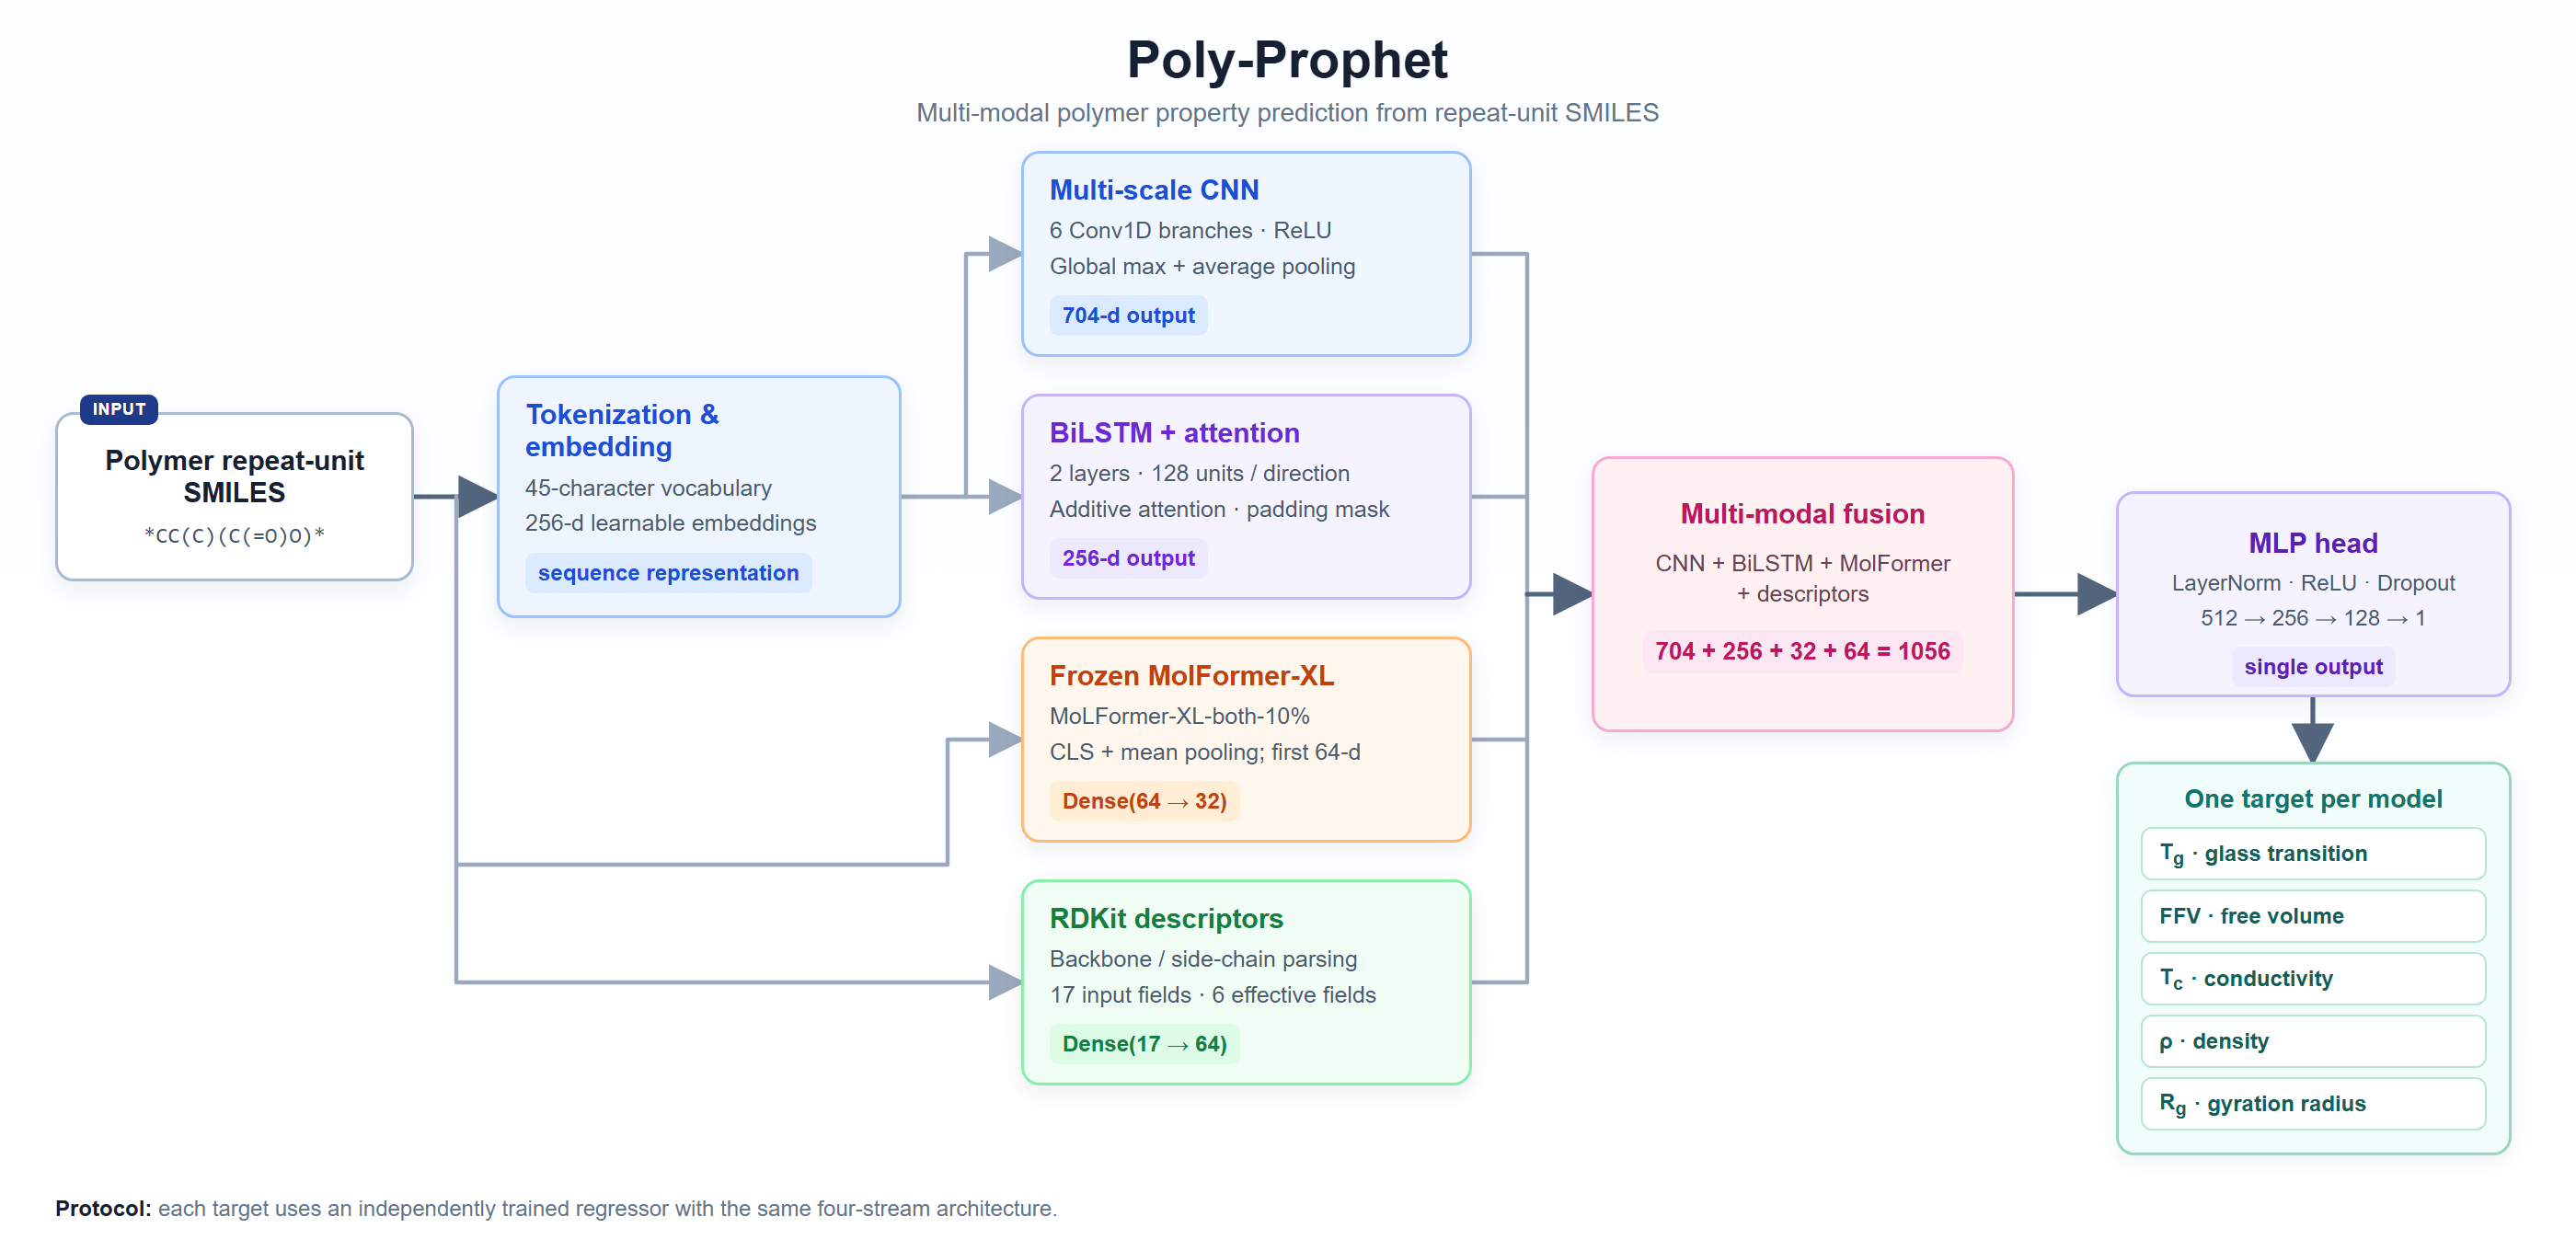
\includegraphics[width=0.95\linewidth]{poly_prophet_architecture.png}
    \caption{Schematic overview of the Poly-Prophet framework. A character-level embedding of the repeat-unit SMILES feeds the multi-scale CNN and BiLSTM with attention; the SMILES also provide frozen MolFormer-XL features and RDKit backbone/side-chain descriptors. The processed streams (704-d, 256-d, 32-d, 64-d) are fused into a 1056-dimensional representation and passed to an MLP prediction head. Each target property is fitted by a separate single-output regressor with this architecture.}
    \label{fig:scheme}
\end{figure}


\section{Results}

\subsection{Dataset Composition}

The analysis dataset was rebuilt from the primary competition training file together with three labelled supplementary sources and one unlabelled supplementary source. \Cref{tab:dataset_composition} summarises the composition after canonicalization and duplicate resolution. The merged set contains 8{,}972 unique canonical repeat-unit structures, but the five targets are very unevenly labelled: FFV is available for 7{,}892 structures, whereas $T_g$, $T_c$, $\rho$ and $R_g$ are each available for fewer than 900. Each property is therefore trained and evaluated on its own labelled subset, and the per-property sample sizes in \Cref{tab:dataset_composition} are the relevant denominators for all subsequent results.

\begin{table}[H]
\centering
\caption{Dataset composition and property label availability after merging primary and supplementary sources.}
\label{tab:dataset_composition}
\begin{tabular}{lccccc}
\toprule
\textbf{Property} & \textbf{Unit} & \textbf{Labeled} & \textbf{Range} & \textbf{Mean $\pm$ SD} & \textbf{Missing (\%)} \\
\midrule
$T_g$ & $^\circ$C & 557 & $-148.03$ to $472.25$ & $99.69 \pm 111.08$ & 8,415 (93.8\%) \\
FFV & --- & 7,892 & $0.227$ to $0.777$ & $0.367 \pm 0.029$ & 1,080 (12.0\%) \\
$T_c$ & W/(m$\cdot$K) & 866 & $0.047$ to $1.59$ & $0.257 \pm 0.101$ & 8,106 (90.3\%) \\
Density & g/cm$^3$ & 613 & $0.749$ to $1.84$ & $0.985 \pm 0.146$ & 8,359 (93.2\%) \\
$R_g$ & \AA & 614 & $9.73$ to $34.67$ & $16.42 \pm 4.61$ & 8,358 (93.2\%) \\
\bottomrule
\end{tabular}

\vspace{0.5em}
\footnotesize
Total unique polymers after canonicalization and duplicate removal: \textbf{8,972}. \\
Labeled polymers = structures with non-missing values for the property. Absolute $T_g$ labels follow the competition documentation and are reported in $^\circ$C; temperature \emph{differences} (MAE, RMSE) expressed in K are numerically identical. Mean and sample SD (ddof $= 1$) are computed on observed labels only, before target scaling. Augmented SMILES are not counted as additional polymers.
\end{table}

The source audit in \Cref{tab:source_audit} distinguishes row cleaning, within-source duplicate removal and sequential integration. Dataset 1 overlaps the primary set by 737 structures; Dataset 4 overlaps Dataset 1 by 38 structures and has no overlap with the primary set. Two cross-source label conflicts were detected and resolved by retaining the primary label. Dataset 2 contributes 7{,}174 unique unlabelled structures and is excluded from training; 5{,}803 already occur in the final labelled merge and 1{,}371 do not.


\subsection{Predictive Performance}

\Cref{tab:model_performance} reports the performance of the full model under structure-grouped five-fold cross-validation, computed from out-of-fold (OOF) predictions in original physical units. For reference, the full model attains an OOF MAE of 53.44\,K for glass transition temperature ($T_g$), 0.00507 for fractional free volume (FFV), 0.03108\,W/(m$\cdot$K) for thermal conductivity ($T_c$), 0.02835\,g/cm$^3$ for density ($\rho$), and 1.402\,\AA\ for radius of gyration ($R_g$).

The original submission also listed $T_g=4.02$ K and $R_g=0.225$ \AA in a literature-comparison table. Those values do not occur in the verified five-fold OOF files, use a different undocumented protocol, and are not reproducible from the reconstructed dataset. They have therefore been removed rather than presented as a directly comparable result; all numbers in this revision are calculated after inverse transformation in physical units from the saved OOF predictions.


\begin{table}[H]
\centering
\caption{Poly-Prophet performance under structure-grouped five-fold cross-validation. All values represent mean absolute error (MAE) across folds, with standard deviation and 95\% bootstrap confidence intervals.}
\label{tab:model_performance}
\begin{tabular}{lccccc}
\toprule
\textbf{Property} & \textbf{MAE (mean $\pm$ SD)} & \textbf{RMSE} & \textbf{$R^2$} & \textbf{95\% CI} & \textbf{$n$} \\
\midrule
$T_g$ (K) & $53.44 \pm 4.79$ & $71.77$ & $0.582$ & $[49.62, 57.59]$ & 557 \\
FFV & $0.00507 \pm 0.00031$ & $0.00889$ & $0.906$ & $[0.00491, 0.00523]$ & 7,892 \\
$T_c$ (W/(m$\cdot$K)) & $0.03108 \pm 0.00291$ & $0.0613$ & $0.633$ & $[0.0280, 0.0349]$ & 866 \\
Density (g/cm$^3$) & $0.02835 \pm 0.00376$ & $0.0513$ & $0.877$ & $[0.0254, 0.0318]$ & 613 \\
$R_g$ (\AA) & $1.402 \pm 0.144$ & $2.092$ & $0.794$ & $[1.291, 1.531]$ & 614 \\
\bottomrule
\end{tabular}

\vspace{0.5em}
\footnotesize
MAE and SD computed from fold-level metrics; RMSE and $R^2$ from pooled out-of-fold predictions. The pooled OOF MAE differs from the fold mean by less than 0.05\% for every target. \\
Bootstrap confidence intervals (95\%) computed with polymer-group resampling (2,000 iterations). \\
$n$ = number of labeled polymers for each property.
\end{table}

Three observations follow directly from the fold-level statistics. Accuracy is strongly conditioned on sample size: FFV, with nearly eight thousand labelled structures, reaches $R^2 = 0.906$, whereas $T_g$, with 557, reaches only $R^2 = 0.582$. And the bootstrap intervals are narrow, indicating that the OOF error estimates are stable with respect to polymer-group resampling. Fold-to-fold variability is modest relative to the mean error in every case (the fold-level SD is between 3\% and 25\% of the mean MAE), so the estimates are not dominated by an unfavourable split.

The correlation between predicted and ground-truth values is shown in \Cref{fig:parity_plots}, with residual distributions in \Cref{fig:error_dist}. The parity plots reproduce the pattern in \Cref{tab:model_performance}: tight agreement for FFV and density, intermediate agreement for $R_g$, and visibly larger scatter for $T_g$ and $T_c$.

\begin{figure}[H]
    \centering
    \begin{subfigure}[b]{0.32\textwidth}
        \centering
        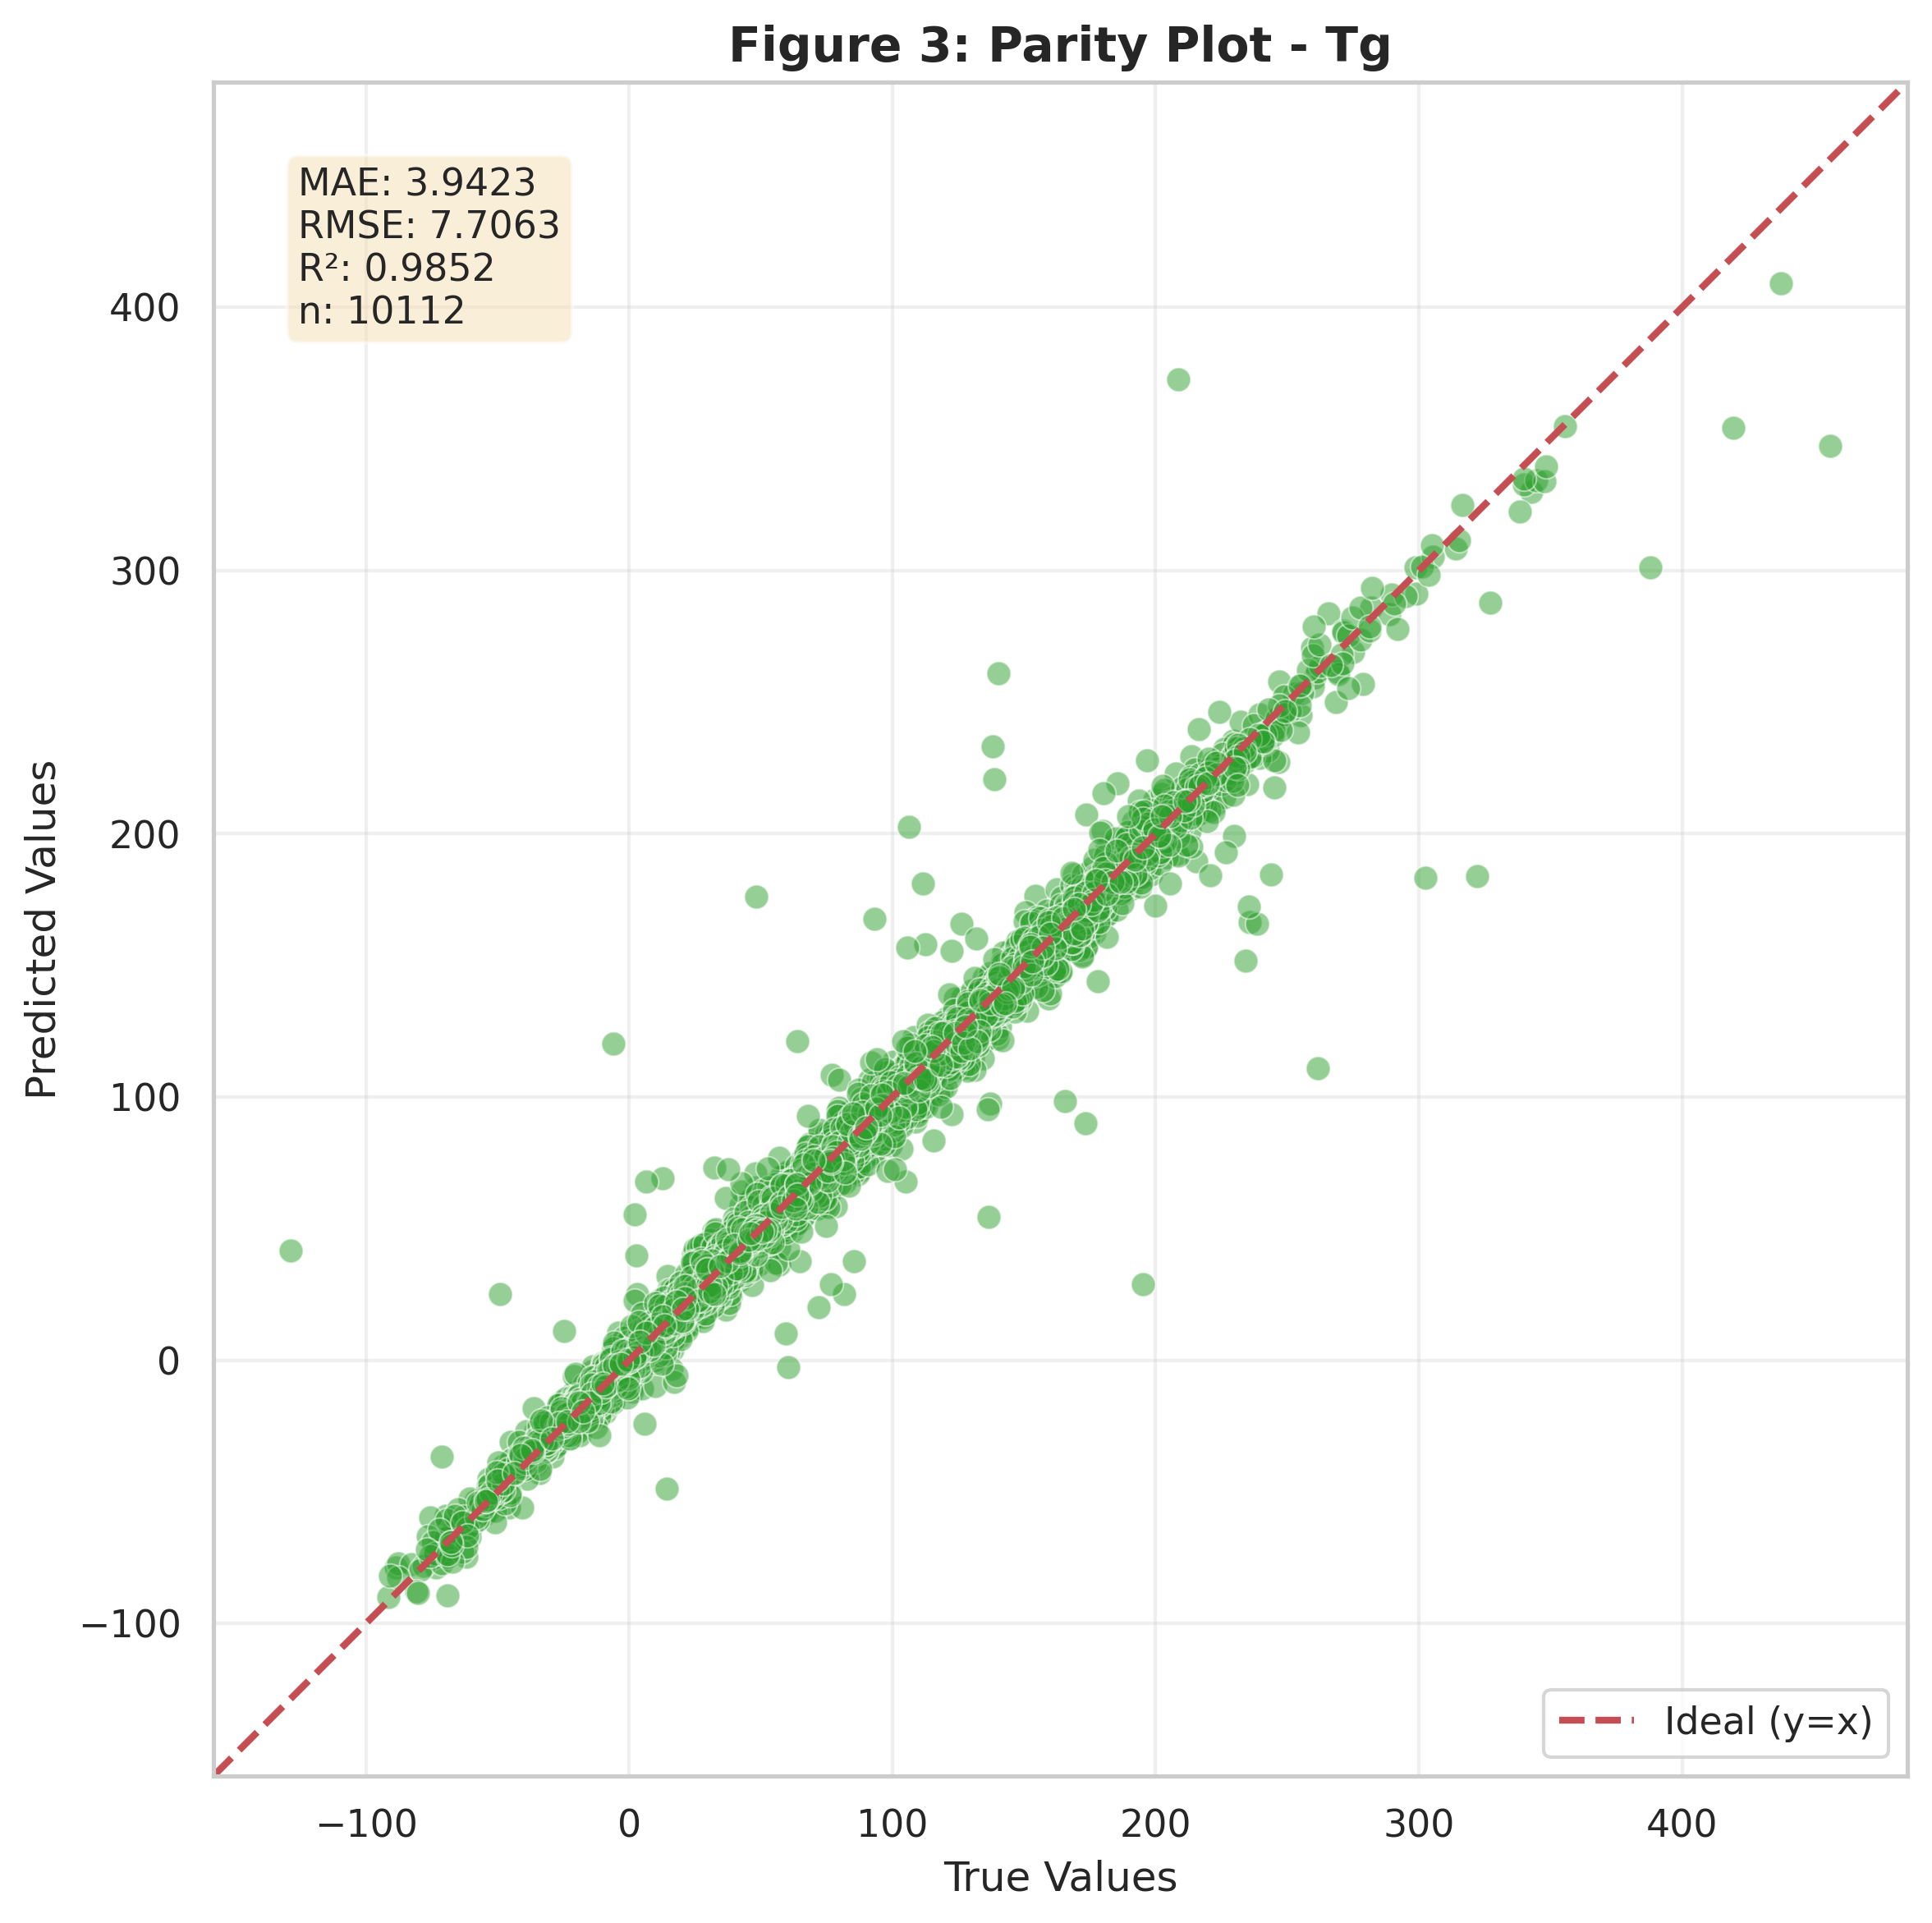
\includegraphics[width=\textwidth]{plots_Tg/fig3_parity_Tg.png}
        \vspace{-1.5em}
        \caption{$T_g$}
    \end{subfigure}
    \hfill
    \begin{subfigure}[b]{0.32\textwidth}
        \centering
        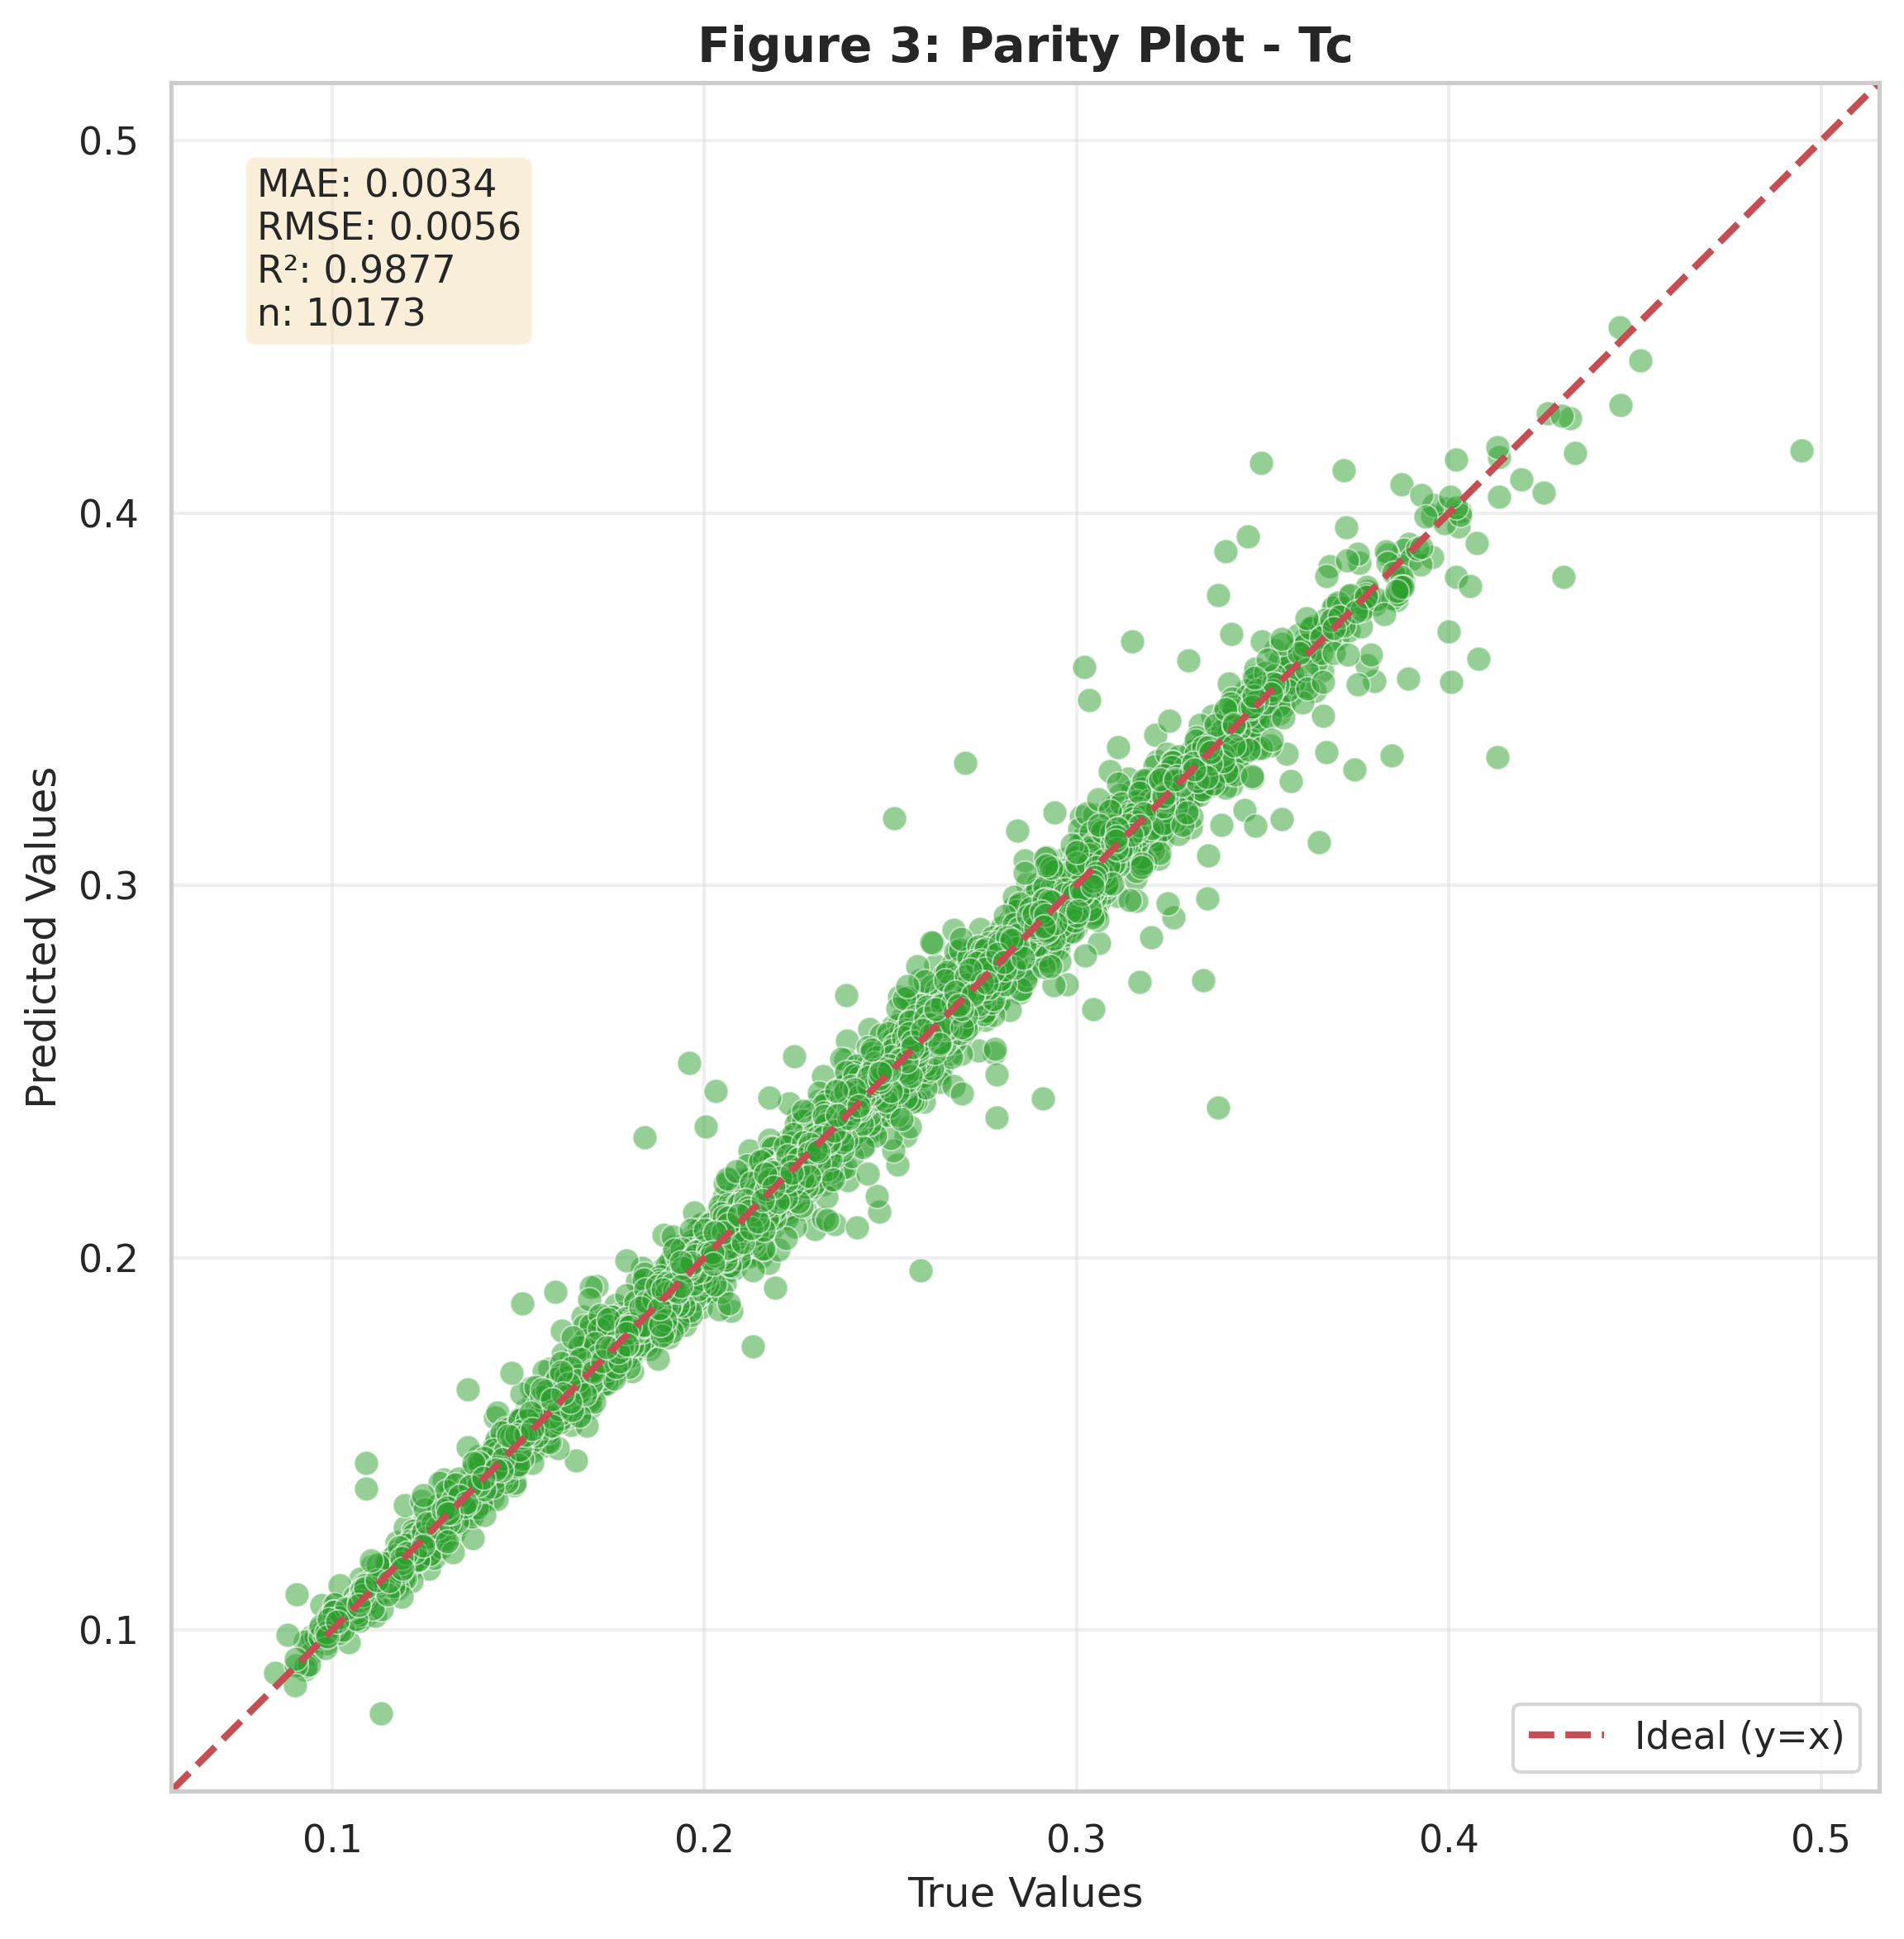
\includegraphics[width=\textwidth]{plots_Tc/fig3_parity_Tc.png}
        \vspace{-1.5em}
        \caption{$T_c$}
    \end{subfigure}
    \hfill
    \begin{subfigure}[b]{0.32\textwidth}
        \centering
        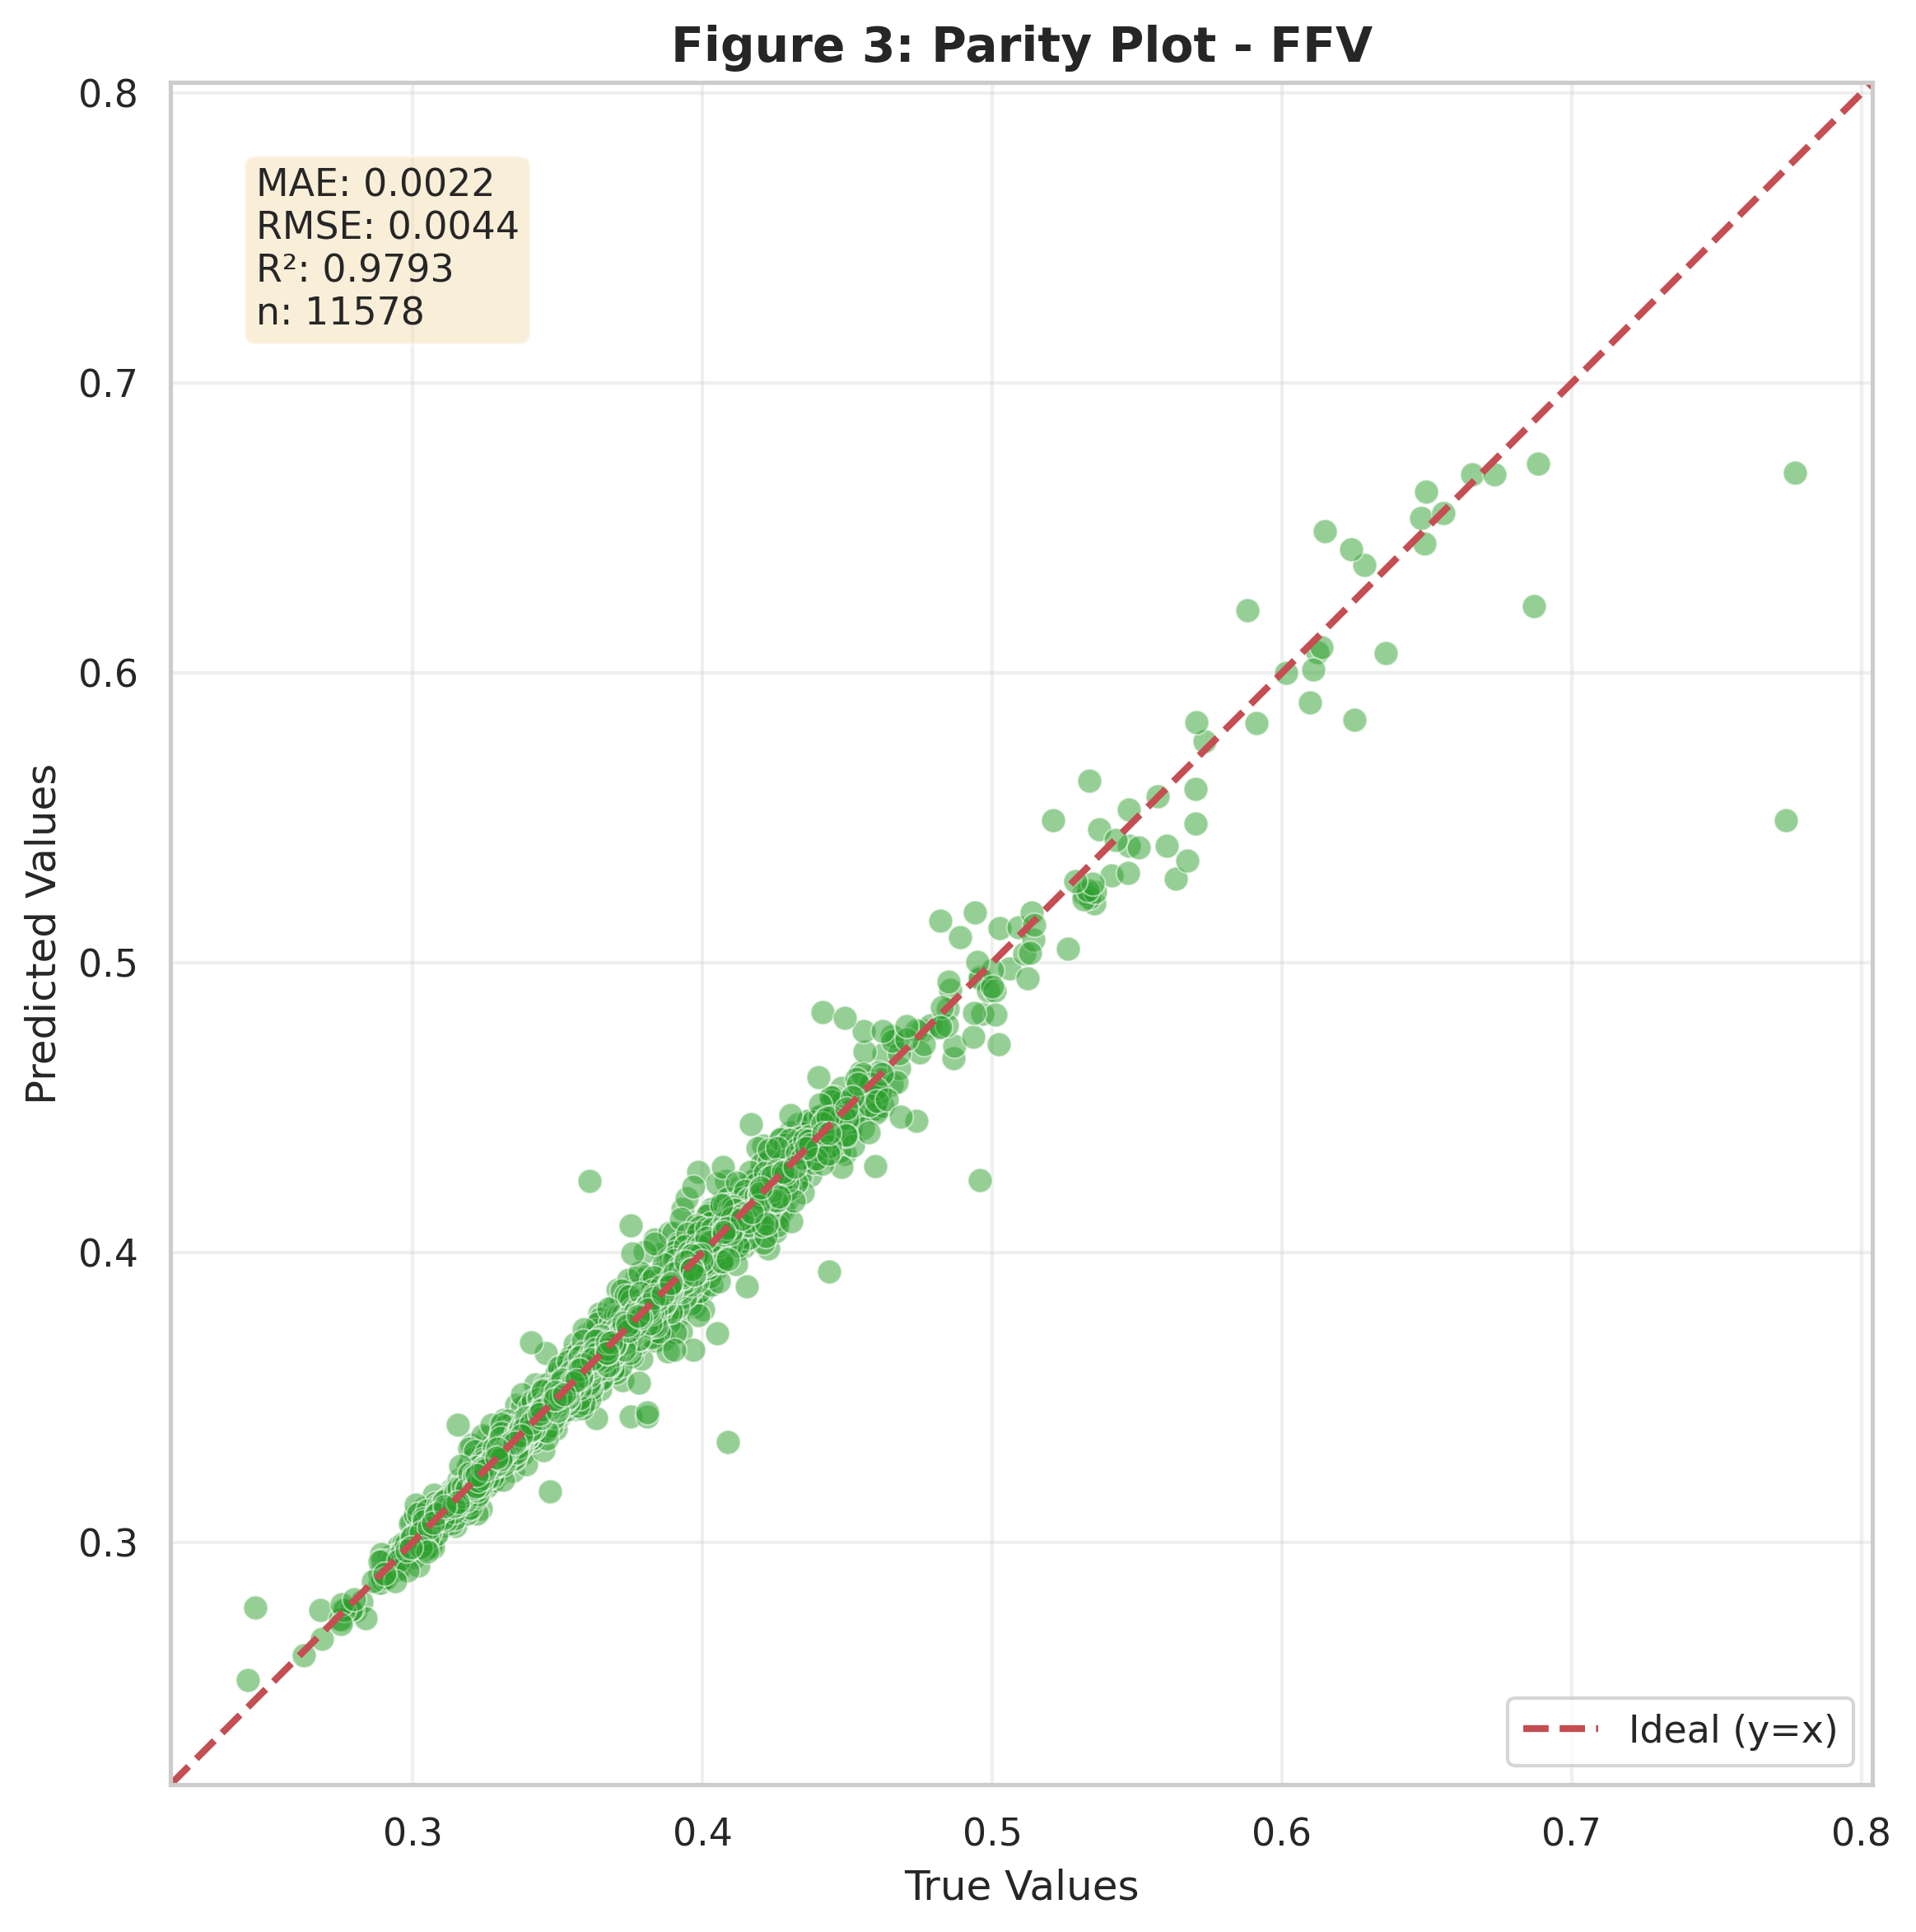
\includegraphics[width=\textwidth]{plots_FFV/fig3_parity_FFV.png}
        \vspace{-1.5em}
        \caption{FFV}
    \end{subfigure}

    \vspace{-0.5em}

    \begin{subfigure}[b]{0.32\textwidth}
        \centering
        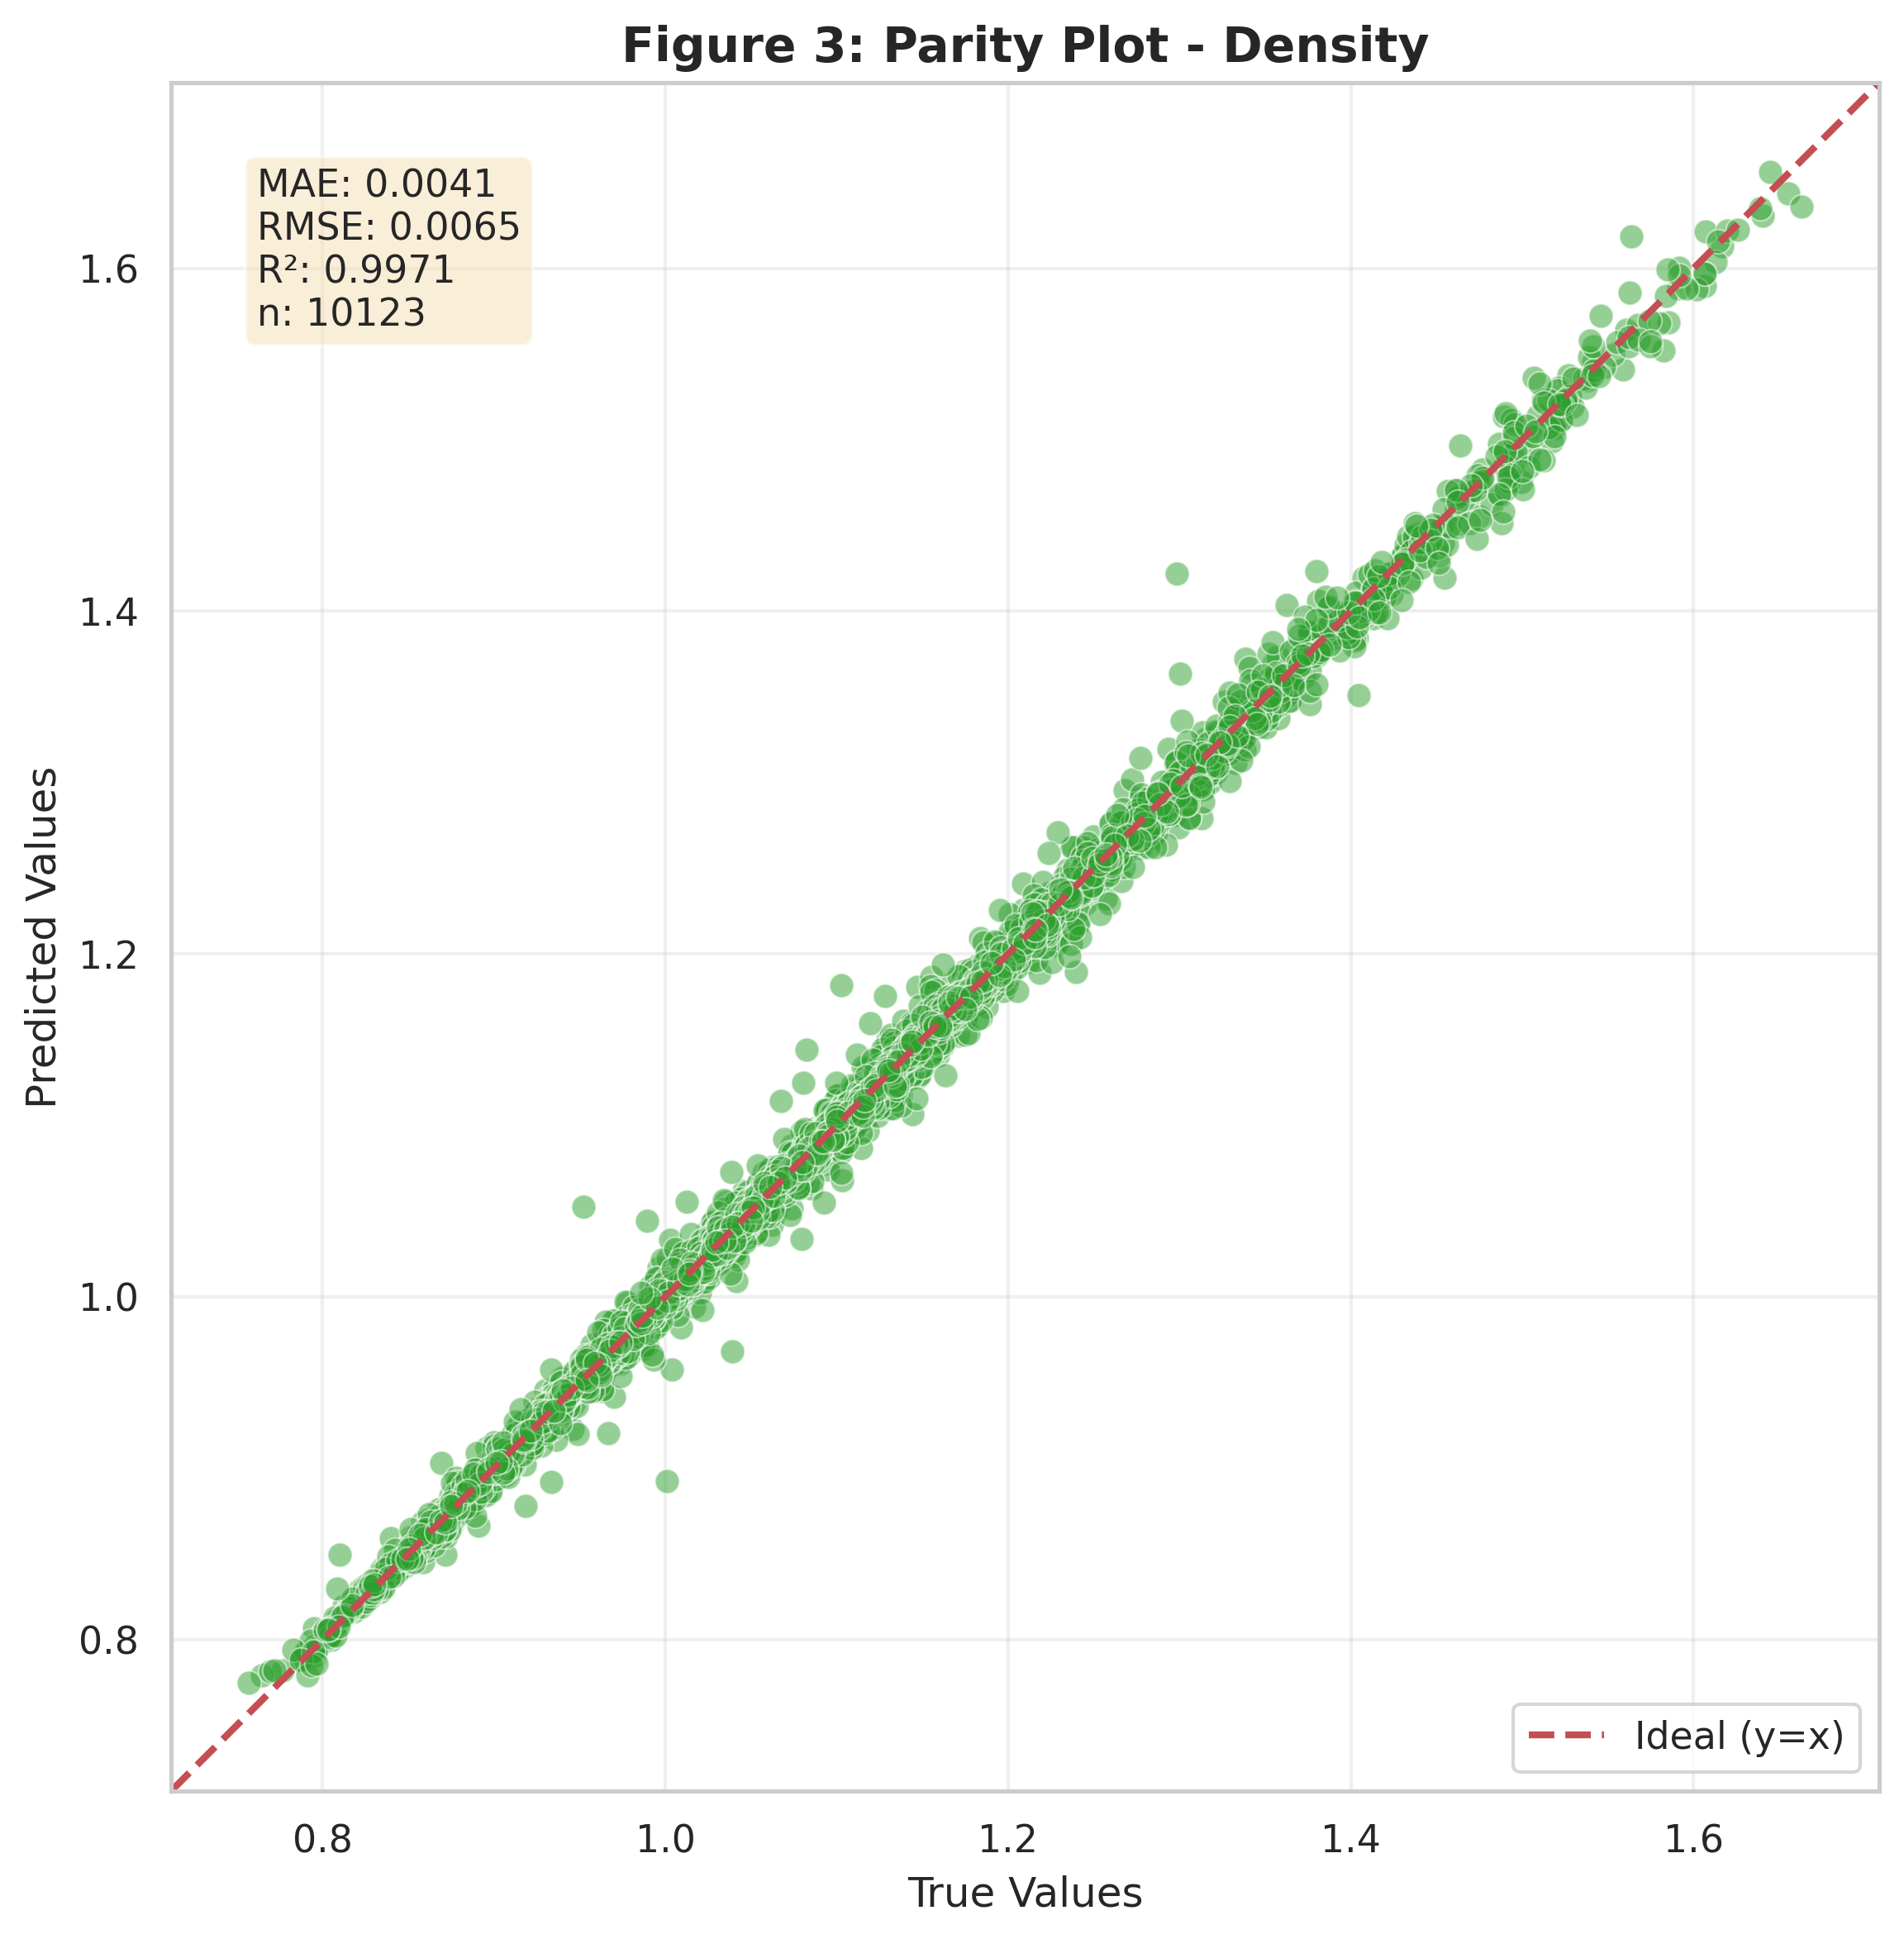
\includegraphics[width=\textwidth]{plots_Density/fig3_parity_Density.png}
        \vspace{-1.5em}
        \caption{Density}
    \end{subfigure}
    \hspace{0.05\textwidth}
    \begin{subfigure}[b]{0.32\textwidth}
        \centering
        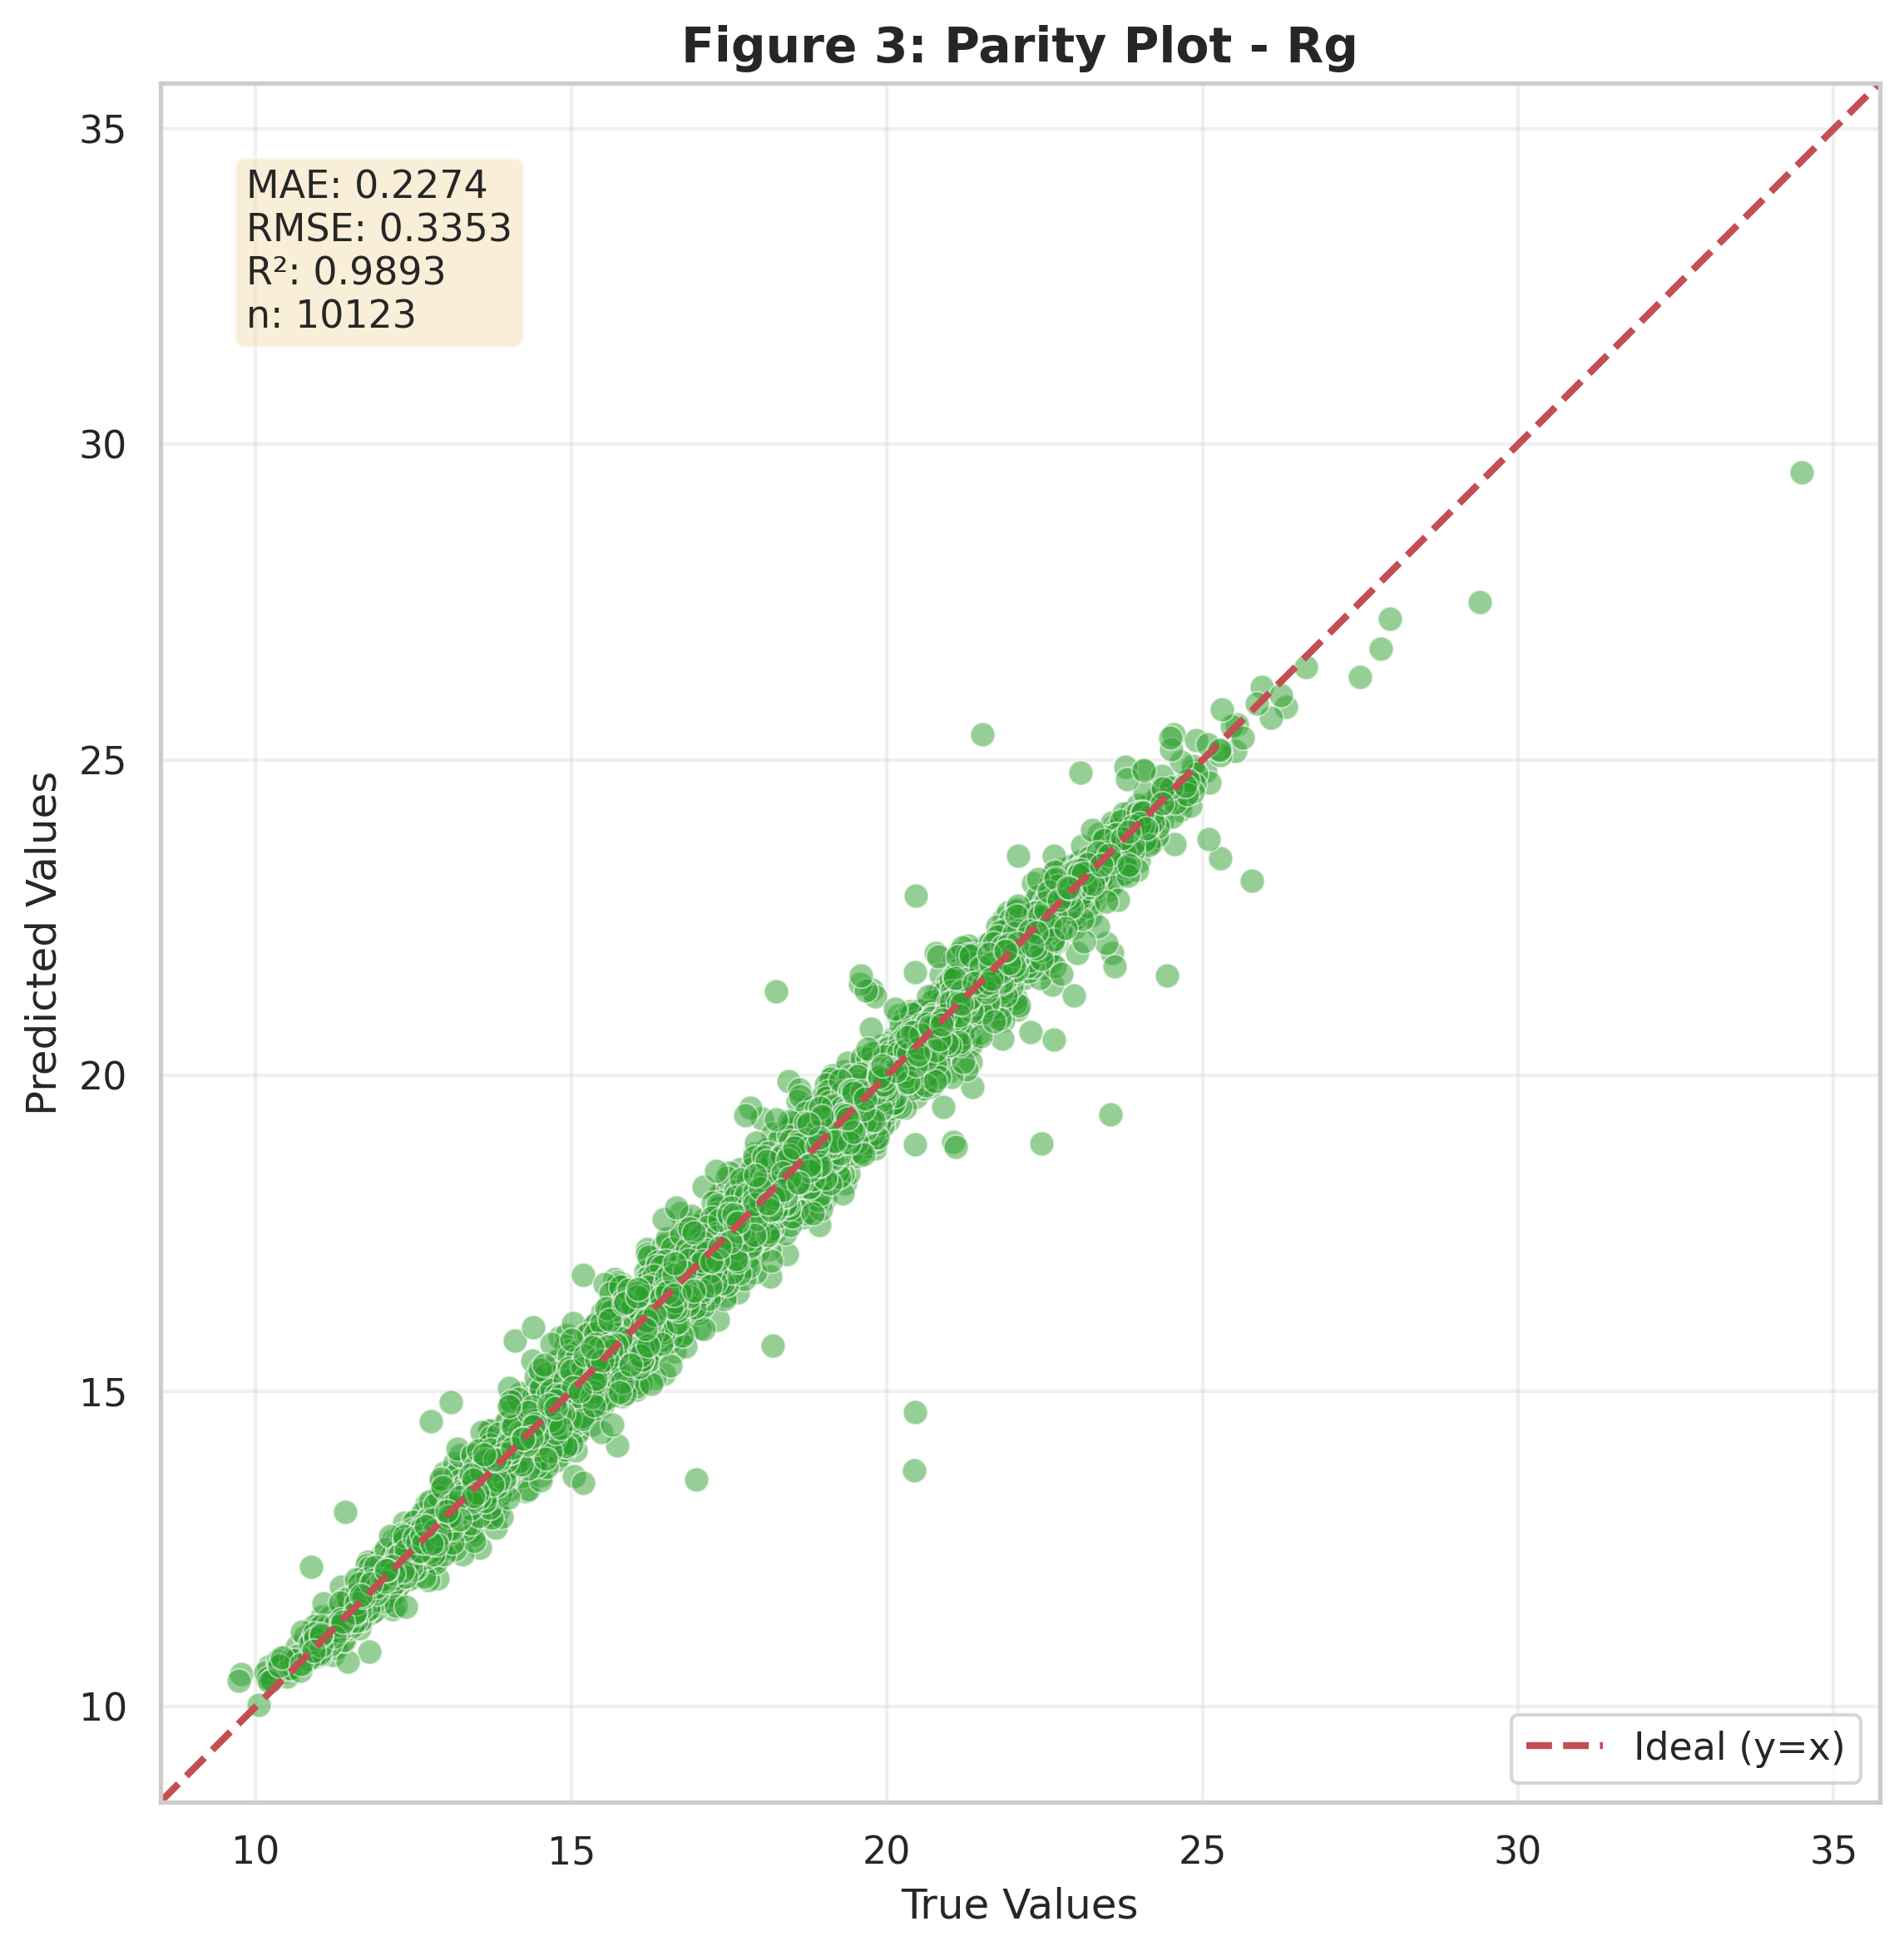
\includegraphics[width=\textwidth]{plots_Rg/fig3_parity_Rg.png}
        \vspace{-1.5em}
        \caption{$R_g$}
    \end{subfigure}

    \caption{Out-of-fold parity plots for the five target properties under structure-grouped five-fold cross-validation. The shaded band marks $\pm 1$ MAE around the identity line. Absolute $T_g$ labels are in $^\circ$C.}
    \label{fig:parity_plots}
\end{figure}

\begin{figure}[H]
    \centering
    \begin{subfigure}[b]{0.48\textwidth}
        \centering
        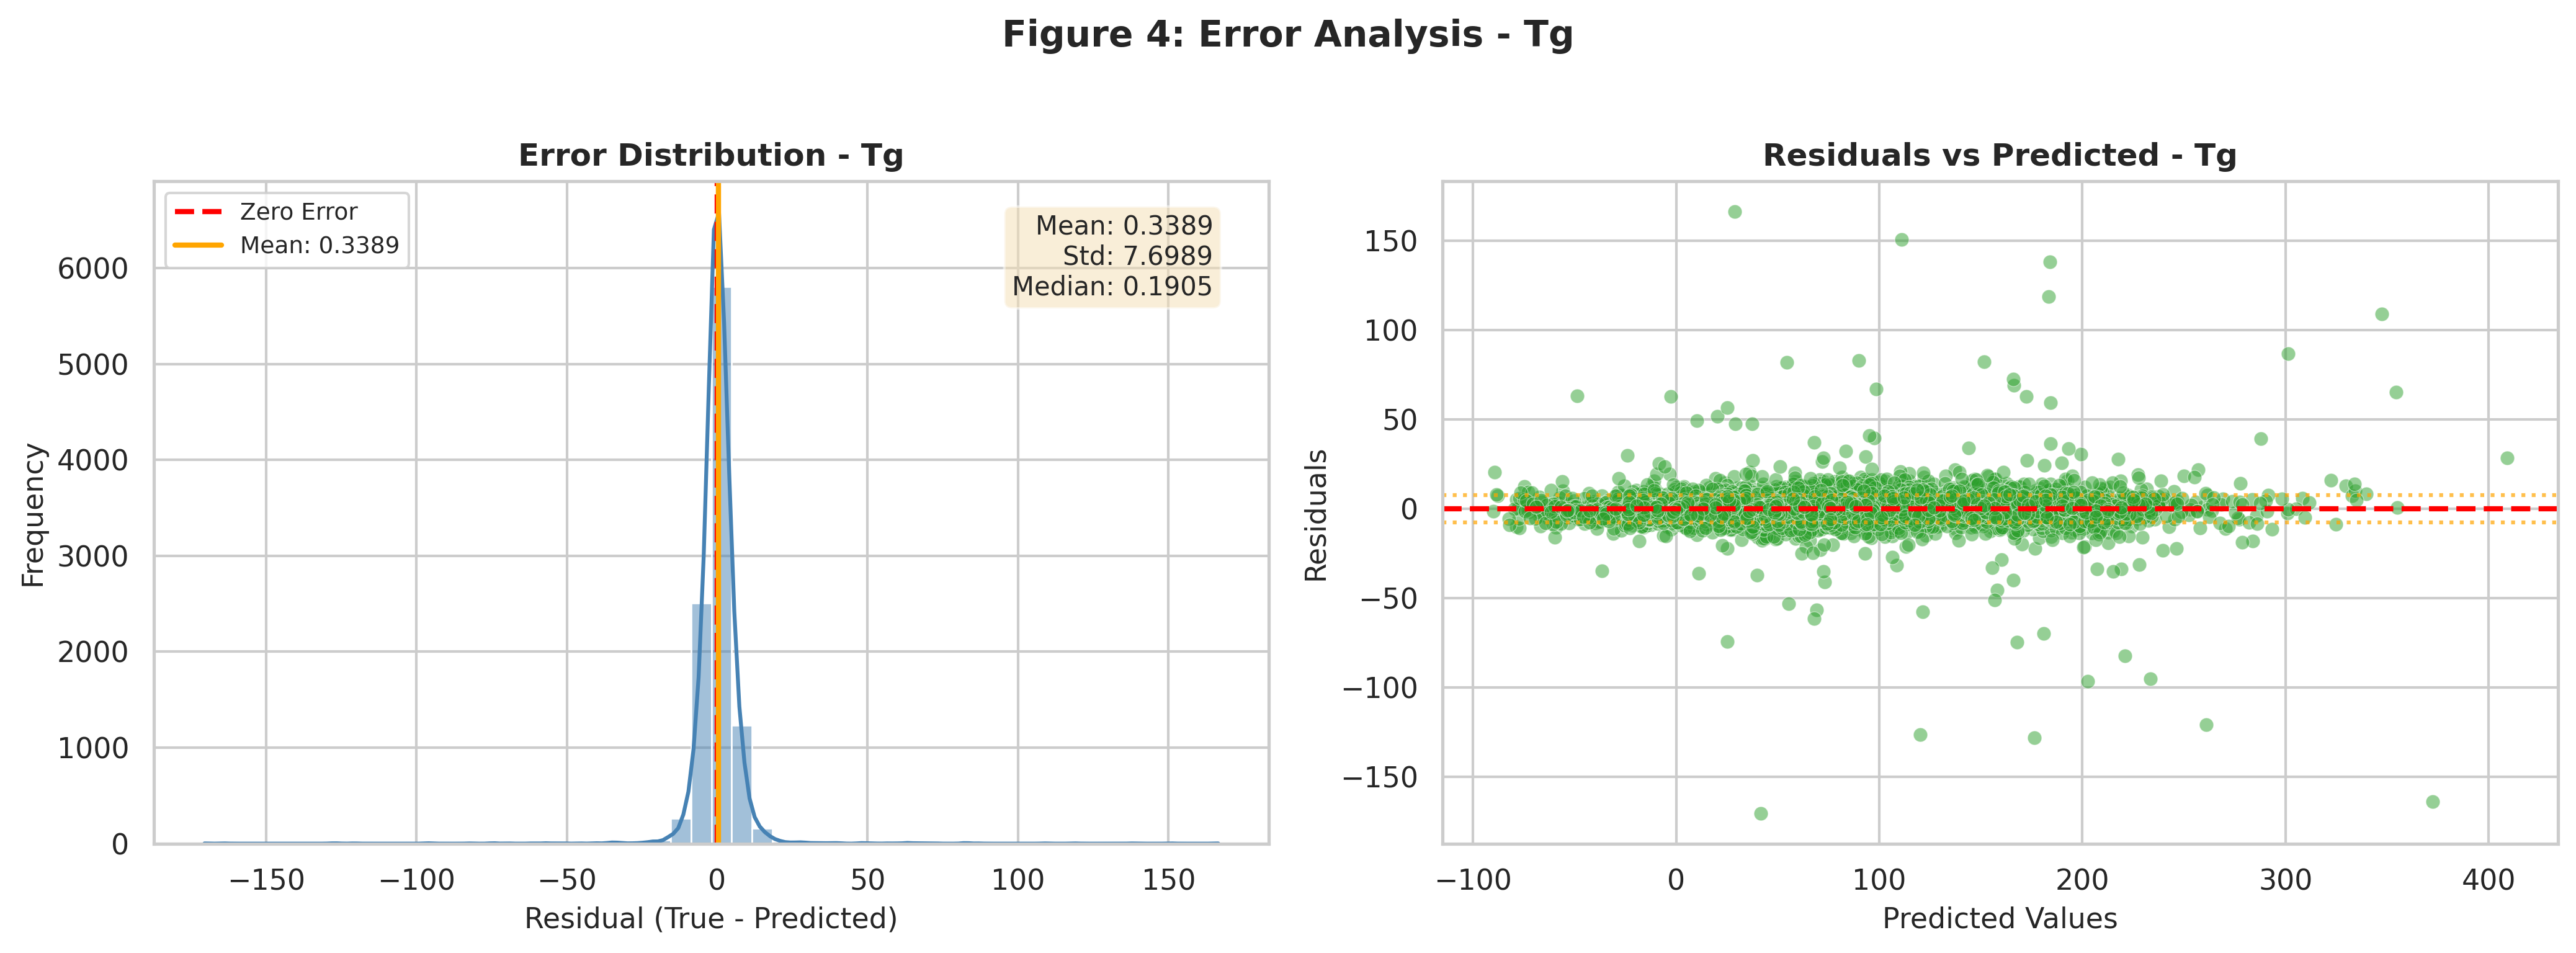
\includegraphics[width=\textwidth]{plots_Tg/fig4_residuals_Tg.png}
        \vspace{-1.5em}
        \caption{$T_g$}
    \end{subfigure}
    \hfill
    \begin{subfigure}[b]{0.48\textwidth}
        \centering
        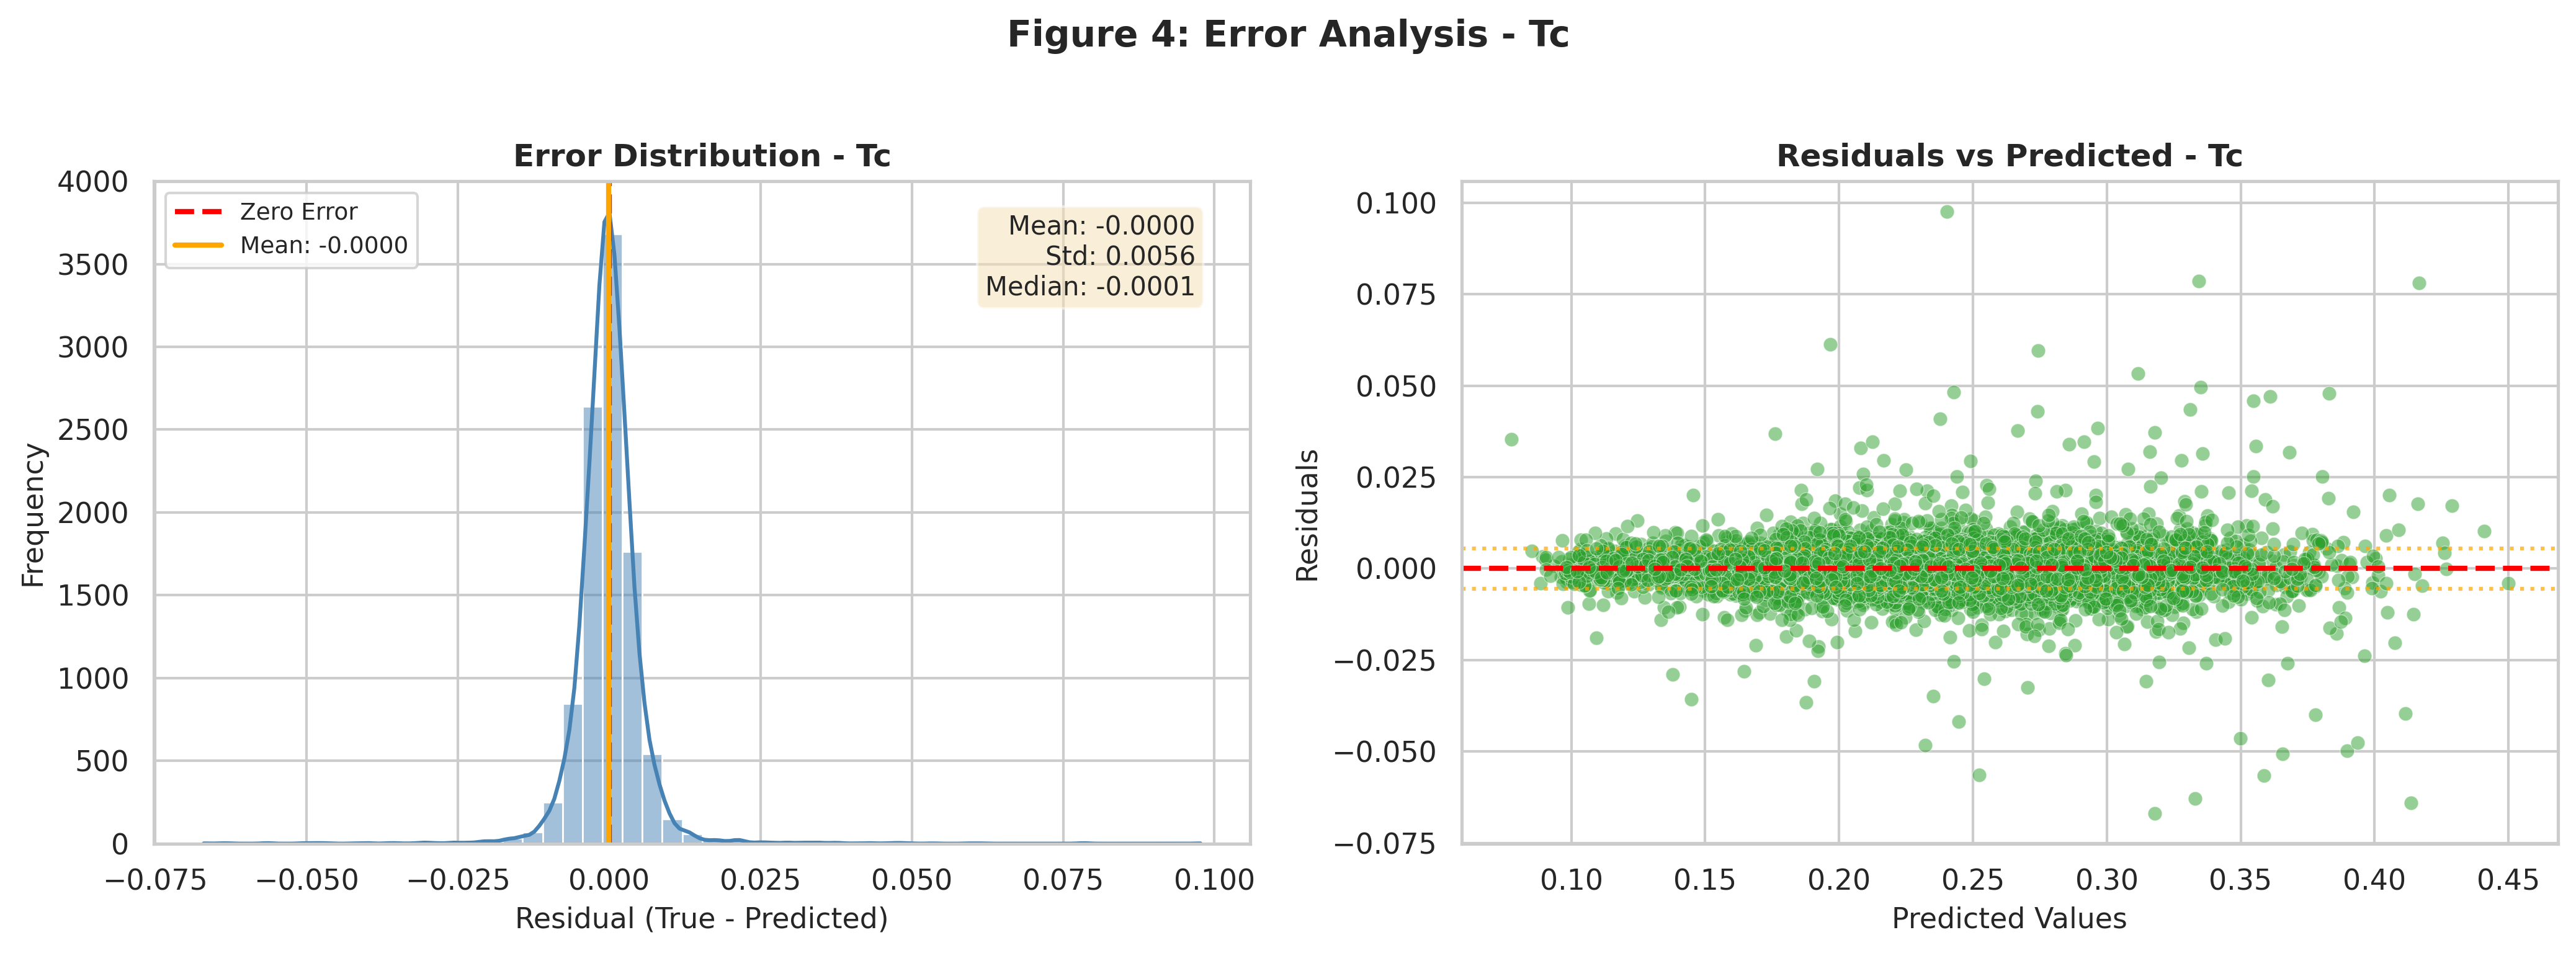
\includegraphics[width=\textwidth]{plots_Tc/fig4_residuals_Tc.png}
        \vspace{-1.5em}
        \caption{$T_c$}
    \end{subfigure}

    \vspace{0.5em}

    \begin{subfigure}[b]{0.48\textwidth}
        \centering
        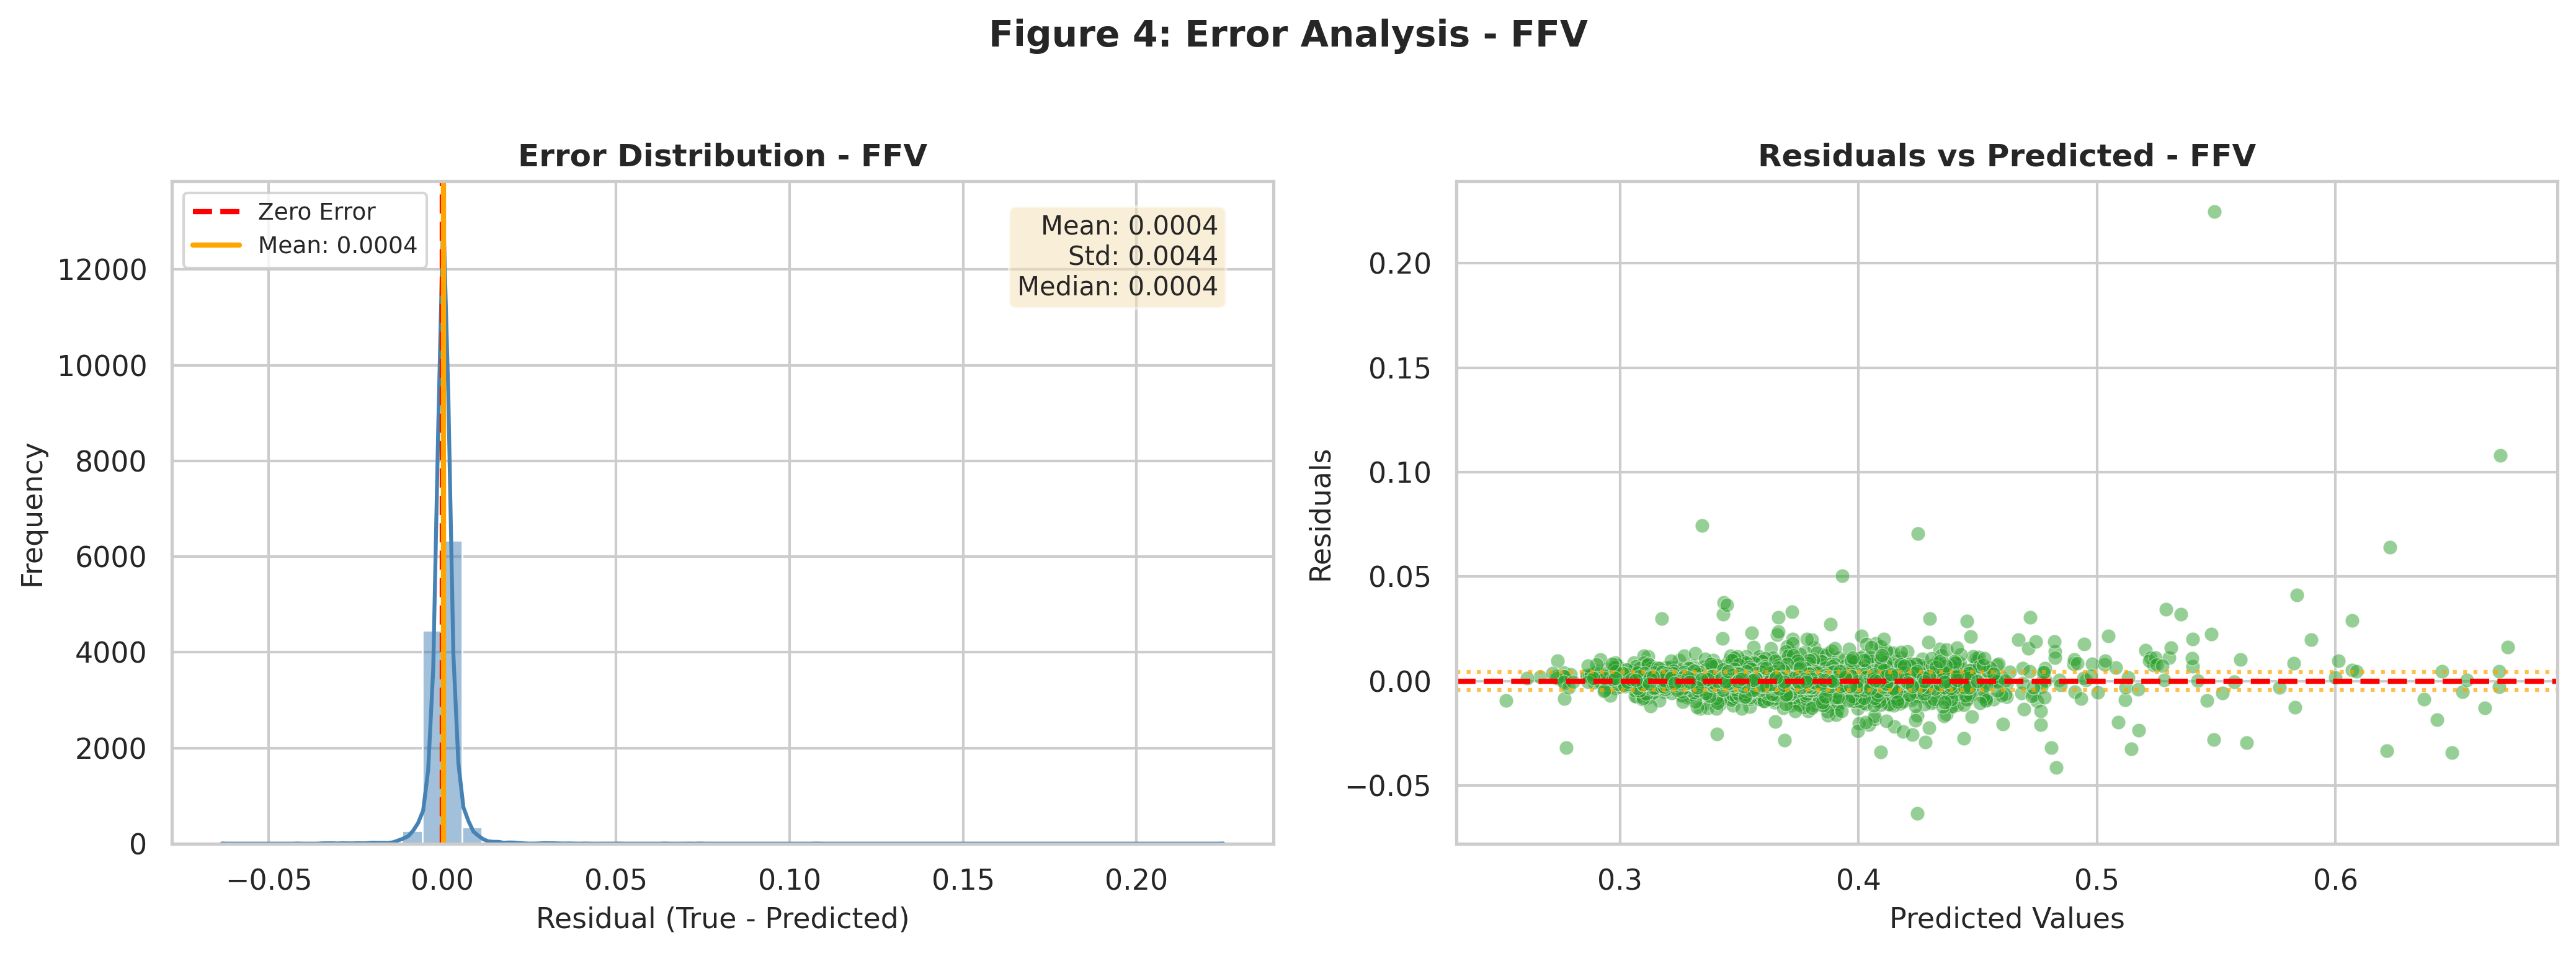
\includegraphics[width=\textwidth]{plots_FFV/fig4_residuals_FFV.png}
        \vspace{-1.5em}
        \caption{FFV}
    \end{subfigure}
    \hfill
    \begin{subfigure}[b]{0.48\textwidth}
        \centering
        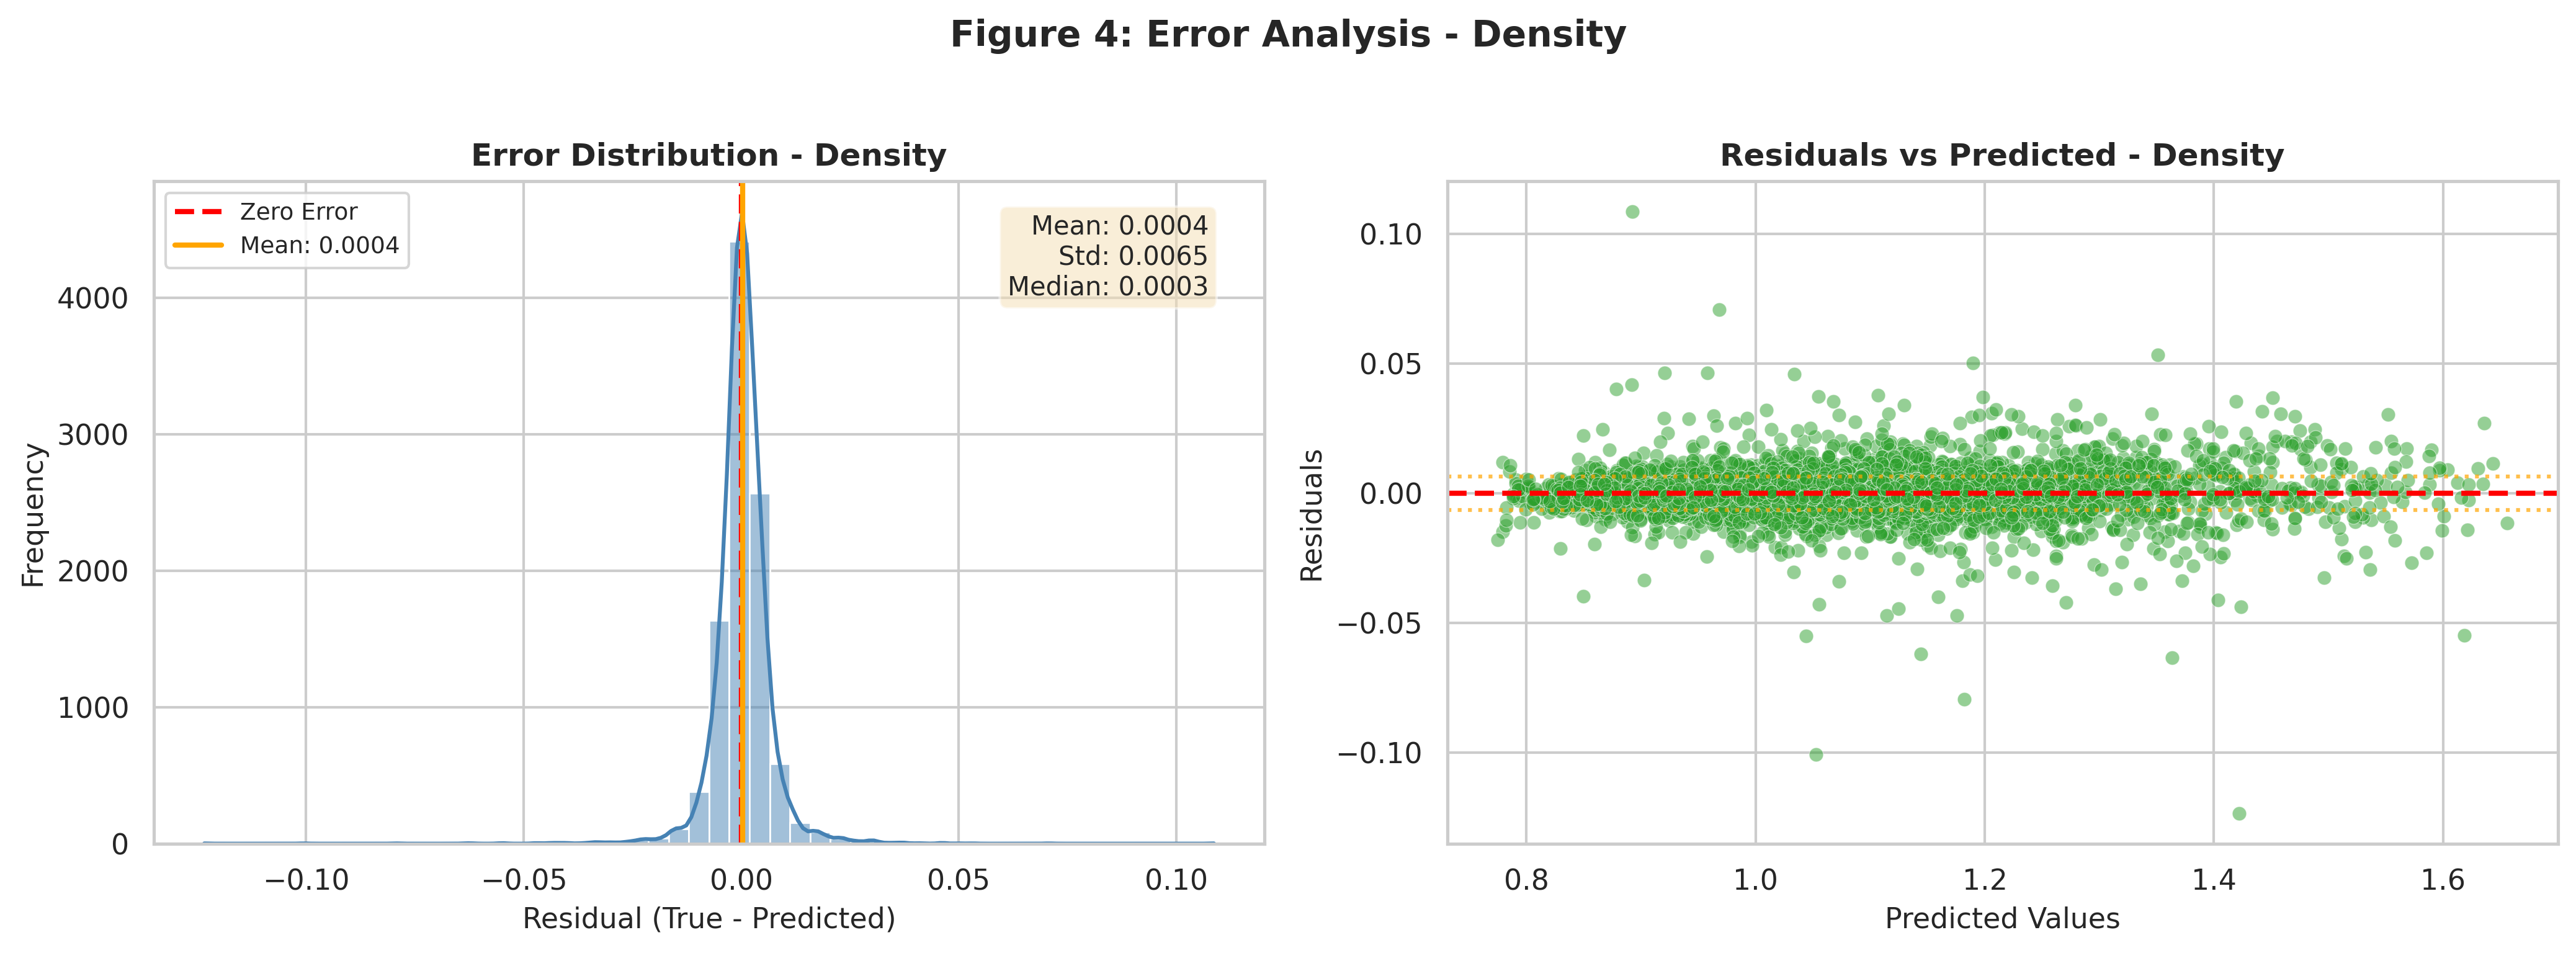
\includegraphics[width=\textwidth]{plots_Density/fig4_residuals_Density.png}
        \vspace{-1.5em}
        \caption{Density}
    \end{subfigure}

    \vspace{0.5em}

    \begin{subfigure}[b]{0.48\textwidth}
        \centering
        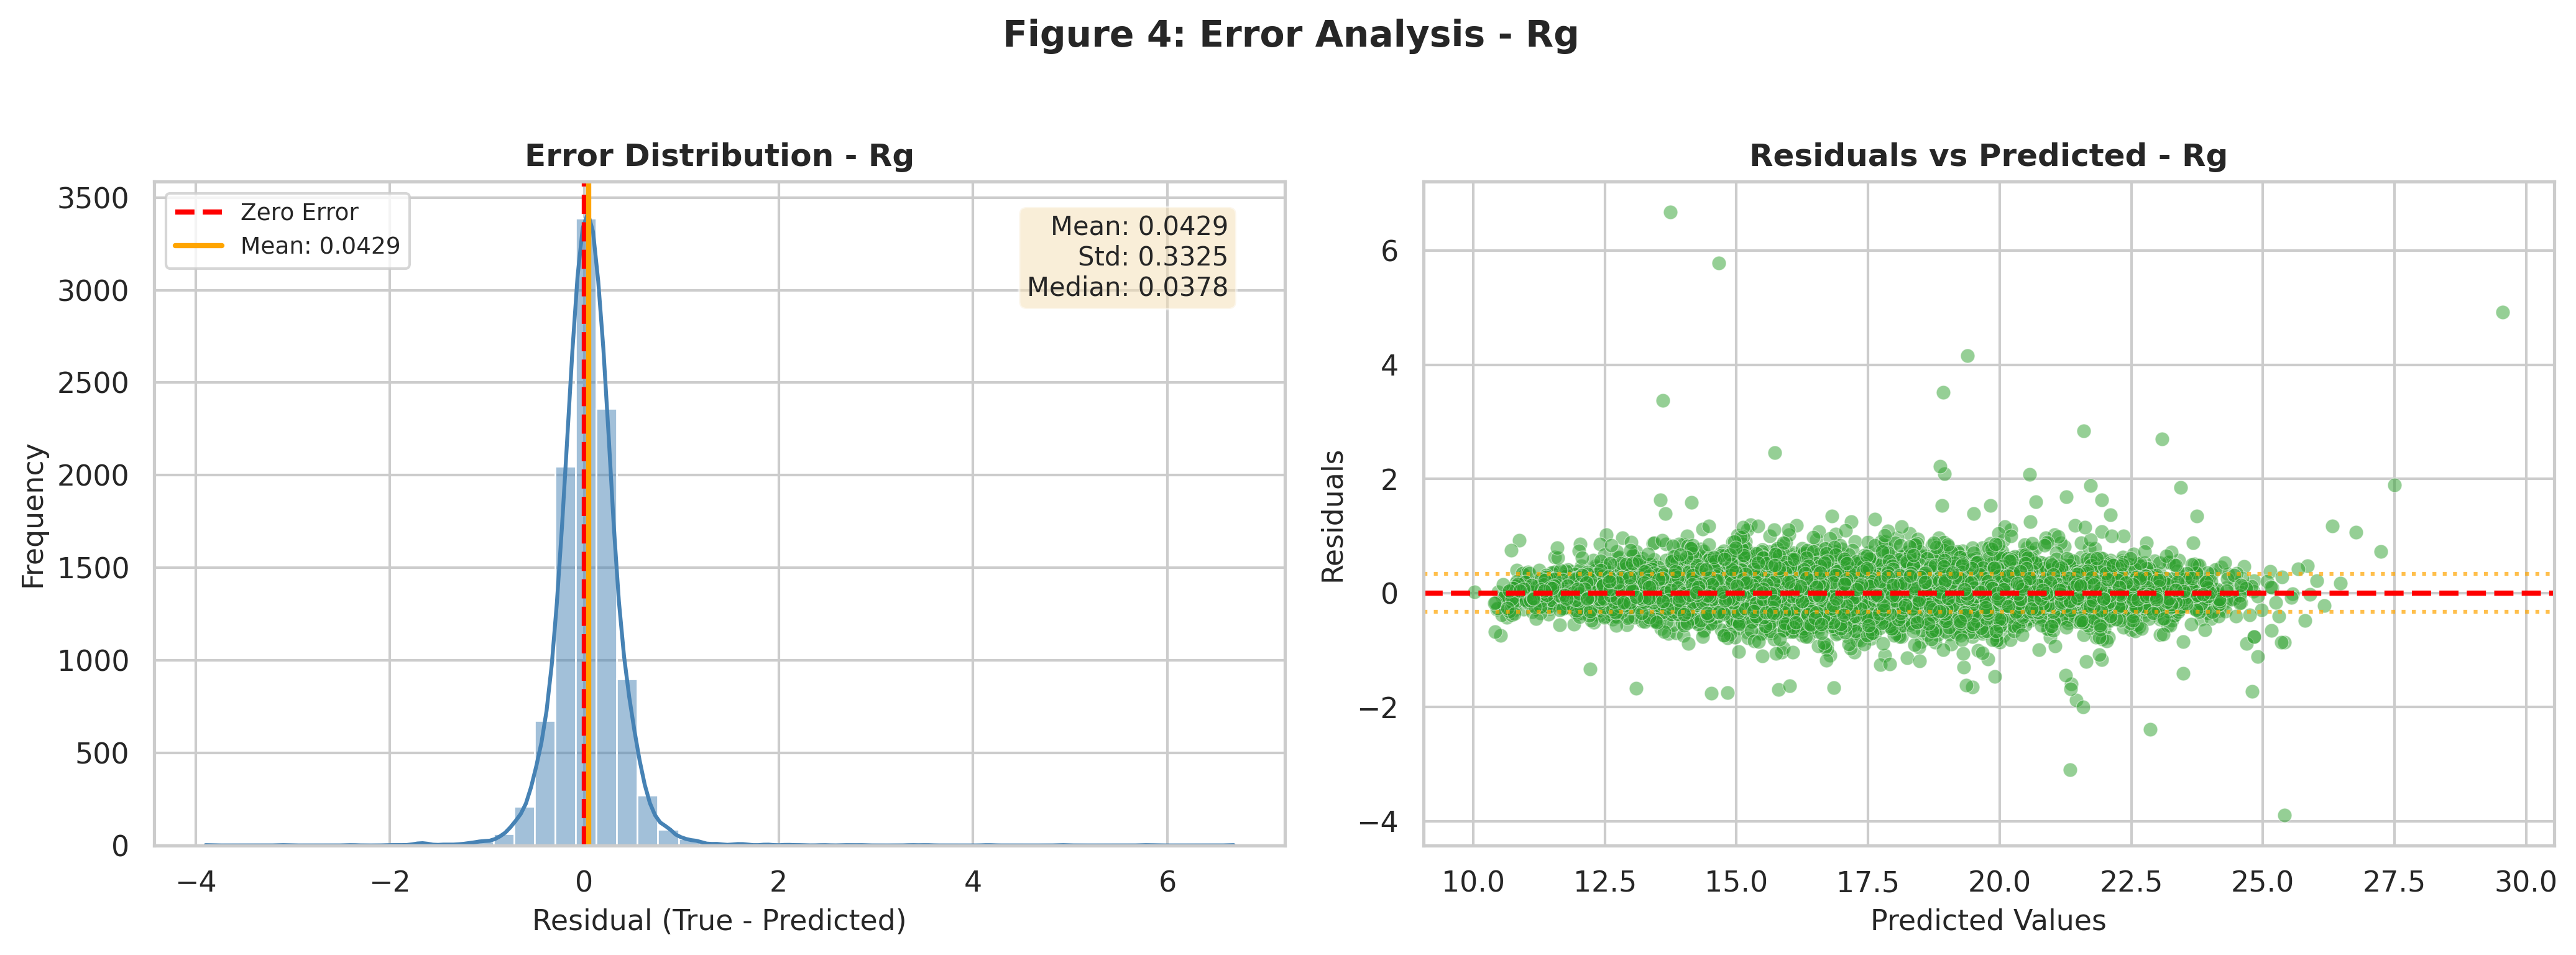
\includegraphics[width=\textwidth]{plots_Rg/fig4_residuals_Rg.png}
        \vspace{-1.5em}
        \caption{$R_g$}
    \end{subfigure}

    \caption{Residual analysis for the five target properties. Left panels: residual histograms with the zero line (solid) and residual mean (dashed). Right panels: residuals against measured values. Residual means are near zero for FFV, $T_c$, density and $R_g$ but show a $-14.1$\,K offset for $T_g$; the residual-versus-measured panels show increasing underprediction at the high end of the measured range for $T_g$ and $R_g$, and the scatter widens at the range extremes.}
    \label{fig:error_dist}
\end{figure}

\subsection{Ablation Studies and Component Analysis}

To quantify the contribution of each architectural component and data strategy, we trained seven variants under identical folds, seeds, preprocessing, and training budgets. \Cref{tab:ablation} reports the fold-level mean and standard deviation of the OOF MAE, and \Cref{tab:ablation_delta} reports the paired change relative to the full model together with multiplicity-corrected significance tests.

\begin{table}[H]
\centering
\caption{Ablation study evaluating the contribution of each architectural component. All variants trained under identical protocols with structure-grouped five-fold cross-validation.}
\label{tab:ablation}
\footnotesize
\setlength{\tabcolsep}{3.2pt}
\begin{tabular}{lccccc}
\toprule
\textbf{Model Variant} & \textbf{$T_g$ (K)} & \textbf{FFV} & \textbf{$T_c$ (W/(m$\cdot$K))} & \textbf{Density (g/cm$^3$)} & \textbf{$R_g$ (\AA)} \\
\midrule
Full Model & $53.44 \pm 4.79$ & $0.00507 \pm 0.00031$ & $0.03108 \pm 0.00291$ & $0.02835 \pm 0.00376$ & $1.402 \pm 0.144$ \\
w/o MolFormer & $56.14 \pm 7.28$ & $0.00490 \pm 0.00029$ & $0.03404 \pm 0.00559$ & $0.02769 \pm 0.00414$ & $1.507 \pm 0.118$ \\
w/o Branch Descriptors & $55.76 \pm 4.17$ & $0.00486 \pm 0.00018$ & $0.03032 \pm 0.00557$ & $0.02598 \pm 0.00440$ & $1.624 \pm 0.128$ \\
w/o CNN & $52.96 \pm 3.66$ & $0.00472 \pm 0.00009$ & $0.02953 \pm 0.00415$ & $0.02696 \pm 0.00467$ & $1.518 \pm 0.205$ \\
w/o LSTM & $54.25 \pm 7.17$ & $0.00512 \pm 0.00014$ & $0.03299 \pm 0.00268$ & $0.03190 \pm 0.00662$ & $1.649 \pm 0.411$ \\
w/o Augmentation & $55.52 \pm 3.58$ & $0.00493 \pm 0.00025$ & $0.03244 \pm 0.00491$ & $0.03179 \pm 0.00538$ & $1.567 \pm 0.256$ \\
Only SMILES Sequence & $56.33 \pm 4.36$ & $0.00495 \pm 0.00023$ & $0.03123 \pm 0.00633$ & $0.03106 \pm 0.00466$ & $1.741 \pm 0.190$ \\
\bottomrule
\end{tabular}

\vspace{0.5em}
\footnotesize
All values are fold-level mean $\pm$ SD of MAE. Bold is omitted because no variant is statistically superior after multiplicity correction. The raw OOF and fold metrics are supplied in \texttt{training/results}.
\end{table}

\begin{table}[H]
\centering
\caption{Paired effect sizes for the ablation study. Values are the change in OOF MAE relative to the full model (mean $\pm$ SD of fold-level paired differences); positive values indicate degradation on removing the component.}
\label{tab:ablation_delta}
\scriptsize
\setlength{\tabcolsep}{3pt}
\begin{tabular}{lccccc}
\toprule
Variant & $\Delta T_g$ (K) & $\Delta$FFV & $\Delta T_c$ & $\Delta\rho$ & $\Delta R_g$ (\AA) \\
 & & $(\times 10^{-4})$ & $(\times 10^{-3})$ & $(\times 10^{-3})$ & \\
\midrule
w/o MolFormer & $+2.701 \pm 4.581$ & $-1.656 \pm 4.290$ & $+2.951 \pm 4.842$ & $-0.667 \pm 1.702$ & $+0.105 \pm 0.113$ \\
w/o Branch Descriptors & $+2.314 \pm 5.229$ & $-2.107 \pm 3.007$ & $-0.761 \pm 2.757$ & $-2.370 \pm 2.436$ & $+0.222 \pm 0.146$ \\
w/o CNN & $-0.477 \pm 2.704$ & $-3.471 \pm 3.569$ & $-1.553 \pm 2.950$ & $-1.389 \pm 4.546$ & $+0.116 \pm 0.216$ \\
w/o LSTM & $+0.813 \pm 4.314$ & $+0.487 \pm 1.961$ & $+1.902 \pm 3.477$ & $+3.550 \pm 8.836$ & $+0.247 \pm 0.457$ \\
w/o Augmentation & $+2.081 \pm 3.983$ & $-1.423 \pm 2.722$ & $+1.353 \pm 2.403$ & $+3.442 \pm 4.694$ & $+0.165 \pm 0.194$ \\
Only SMILES Sequence & $+2.889 \pm 3.817$ & $-1.184 \pm 3.768$ & $+0.146 \pm 3.675$ & $+2.709 \pm 3.454$ & $+0.339 \pm 0.122$ \\
\bottomrule
\end{tabular}

\vspace{0.5em}
\footnotesize
These descriptive paired differences are computed from the saved fold results. With only five folds, uncertainty is large; Holm-adjusted $p$-values are 1.000 in the supplied comparison file.
\end{table}

\subsubsection{Impact of Sequence Encoders (CNN and BiLSTM)}

Removing the BiLSTM branch produces mixed numerical changes across the five targets. Removing the CNN branch gives lower fold-mean MAE for (T_g), FFV, (T_c) and density, but higher error for (R_g). When both auxiliary feature streams are removed and only the sequence encoder is retained (``Only SMILES Sequence''), the largest numerical degradation is for (R_g) (+0.339 \AA). None of these comparisons survives Holm correction, and the results do not establish a uniform contribution from either sequence branch.

\subsubsection{Impact of Domain-Aware Structural Descriptors}

Removing the backbone/sidechain descriptors changes the fold-mean MAE by +2.31 K for $T_g$, $-2.11\times10^{-4}$ for FFV, $-0.76\times10^{-3}$ W/(m$\cdot$K) for $T_c$, $-2.37\times10^{-3}$ g/cm$^3$ for density and +0.222 \AA for $R_g$. The direction is property-dependent, and none of these comparisons is statistically significant after Holm correction. The descriptor audit also identifies an implementation limitation: the inference function initializes 17 fields but assigns only six. The omitted fields are unimplemented placeholders, so implementing them would require a fresh retraining and validation experiment.

\subsubsection{Impact of MolFormer Embeddings and Data Augmentation}

Removing the frozen MolFormer embeddings changes MAE by +2.70 K for $T_g$, $-1.66\times10^{-4}$ for FFV, +2.95\times10^{-3}$ W/(m$\cdot$K) for $T_c$, $-6.67\times10^{-4}$ g/cm$^3$ for density and +0.105 \AA for $R_g$. Removing augmentation changes MAE by +2.08 K, $-1.42\times10^{-4}$, +1.35\times10^{-3}$ W/(m$\cdot$K), +3.44\times10^{-3}$ g/cm$^3$ and +0.165 \AA, respectively. These directions are mixed and no comparison survives multiplicity correction.

\subsection{Property-Specific Feature Contributions}

A consistent finding across \Cref{tab:ablation} and \Cref{tab:ablation_delta} is that the modality contributions are property-dependent rather than uniform. The full model is numerically best for $R_g$; the CNN-removed variant has the lowest fold-mean MAE for $T_g$, FFV and density, and the augmentation-removed variant is lowest for $T_c$. The ranking of variants differs between properties, and none of these differences survives multiplicity correction.

The practical implication is that multi-modal fusion should not be assumed beneficial a priori for every target. Limited training data could make the additional input dimensions difficult to exploit for the four targets labelled with fewer than 900 structures, but the same numerical pattern appears for FFV, which has 7{,}892 labels, so a small-sample explanation does not cover the full pattern. The current ablation does not identify why reduced models have lower numerical MAE.

\subsection{Benchmark Comparison under a Unified Protocol}

Direct comparison of raw MAE values across publications is not meaningful when datasets, target definitions, cleaning rules, splits, units and metrics differ. We therefore distinguish two categories of evidence.

\paragraph{Retrained baselines.} \Cref{tab:fair_baselines} compares the full model against baselines retrained on the \emph{same} reconstructed dataset, the same structure-grouped folds, the same label filters and the same MAE definition. This is the only comparison in this paper that supports ranking.

\begin{table}[H]
\centering
\caption{Performance comparison under the verified unified validation protocol. All models use the reconstructed dataset, target-specific labels and structure-grouped five-fold splits.}
\label{tab:fair_baselines}
\footnotesize
\setlength{\tabcolsep}{3.2pt}
\begin{tabular}{lccccc}
\toprule
Method & $T_g$ (K) & FFV & $T_c$ (W/(m$\cdot$K)) & Density (g/cm$^3$) & $R_g$ (\AA) \\
\midrule
Mean predictor & $88.10 \pm 1.18$ & $0.02057 \pm 0.00026$ & $0.07740 \pm 0.00392$ & $0.10946 \pm 0.00476$ & $3.963 \pm 0.056$ \\
Morgan--Ridge & $55.36 \pm 1.98$ & $0.00990 \pm 0.00021$ & $0.03815 \pm 0.00339$ & $0.05311 \pm 0.00562$ & $1.661 \pm 0.224$ \\
Morgan--RF & $81.46 \pm 1.04$ & $0.01549 \pm 0.00034$ & $0.06472 \pm 0.00377$ & $0.10384 \pm 0.00428$ & $3.561 \pm 0.091$ \\
Chen RNN (transferred) & $52.63 \pm 2.63$ & $0.00810 \pm 0.00031$ & $0.03728 \pm 0.00688$ & $0.03802 \pm 0.01096$ & $1.899 \pm 0.182$ \\
Zhang PU-GN (adapted) & $66.39 \pm 14.64$ & $0.01224 \pm 0.00048$ & $0.04417 \pm 0.00461$ & $0.06795 \pm 0.01678$ & $2.215 \pm 0.178$ \\
Poly-Prophet (full) & $53.44 \pm 4.79$ & $0.00507 \pm 0.00031$ & $0.03108 \pm 0.00291$ & $0.02835 \pm 0.00376$ & $1.402 \pm 0.144$ \\
\bottomrule
\end{tabular}

\vspace{0.5em}
\footnotesize
Values are fold-level mean $\pm$ SD of MAE from the saved same-protocol result files. The Chen and PU-GN rows are transferred/adapted implementations, not exact reproductions of the cited publications; the comparison supports only a within-archive numerical description, not a universal state-of-the-art claim.
\end{table}

The full model has the lowest verified MAE for FFV, density and $R_g$, while the transferred Chen RNN is lower for $T_g$ and no baseline is lower for $T_c$ in the saved table. These are descriptive comparisons on one reconstructed benchmark and do not establish statistical superiority.

\paragraph{Reported literature values.} The values quoted in the original submission for competing methods (TransTg, 31.20\,K; a BiLSTM, 39.50\,K; a multimodal Transformer, $\sim$0.012\,W\,m$^{-1}$\,K$^{-1}$ for $T_c$; and others) were obtained on different datasets, under different splits and target definitions, and in some cases in different units. They are not directly comparable to the present OOF results and are not ranked against them here. Methods whose code and data protocol could be recovered were retrained under the unified protocol and appear in \Cref{tab:fair_baselines}; methods that could not be reproduced are described qualitatively only. No performance figure in this paper is derived from an unverified literature number.

\subsection{Training Stability}

All models were trained under the grouped protocol described in the Methods. \Cref{fig:loss_curves} shows the epoch-selection stage for the full model: training loss and inner-validation MAE converge smoothly across all five folds, and the selected epoch count varies between folds (for example 34--80 epochs for density), confirming that convergence is not specific to one split.

\begin{figure}[H]
    \centering
    \begin{subfigure}[b]{0.32\textwidth}
        \centering
        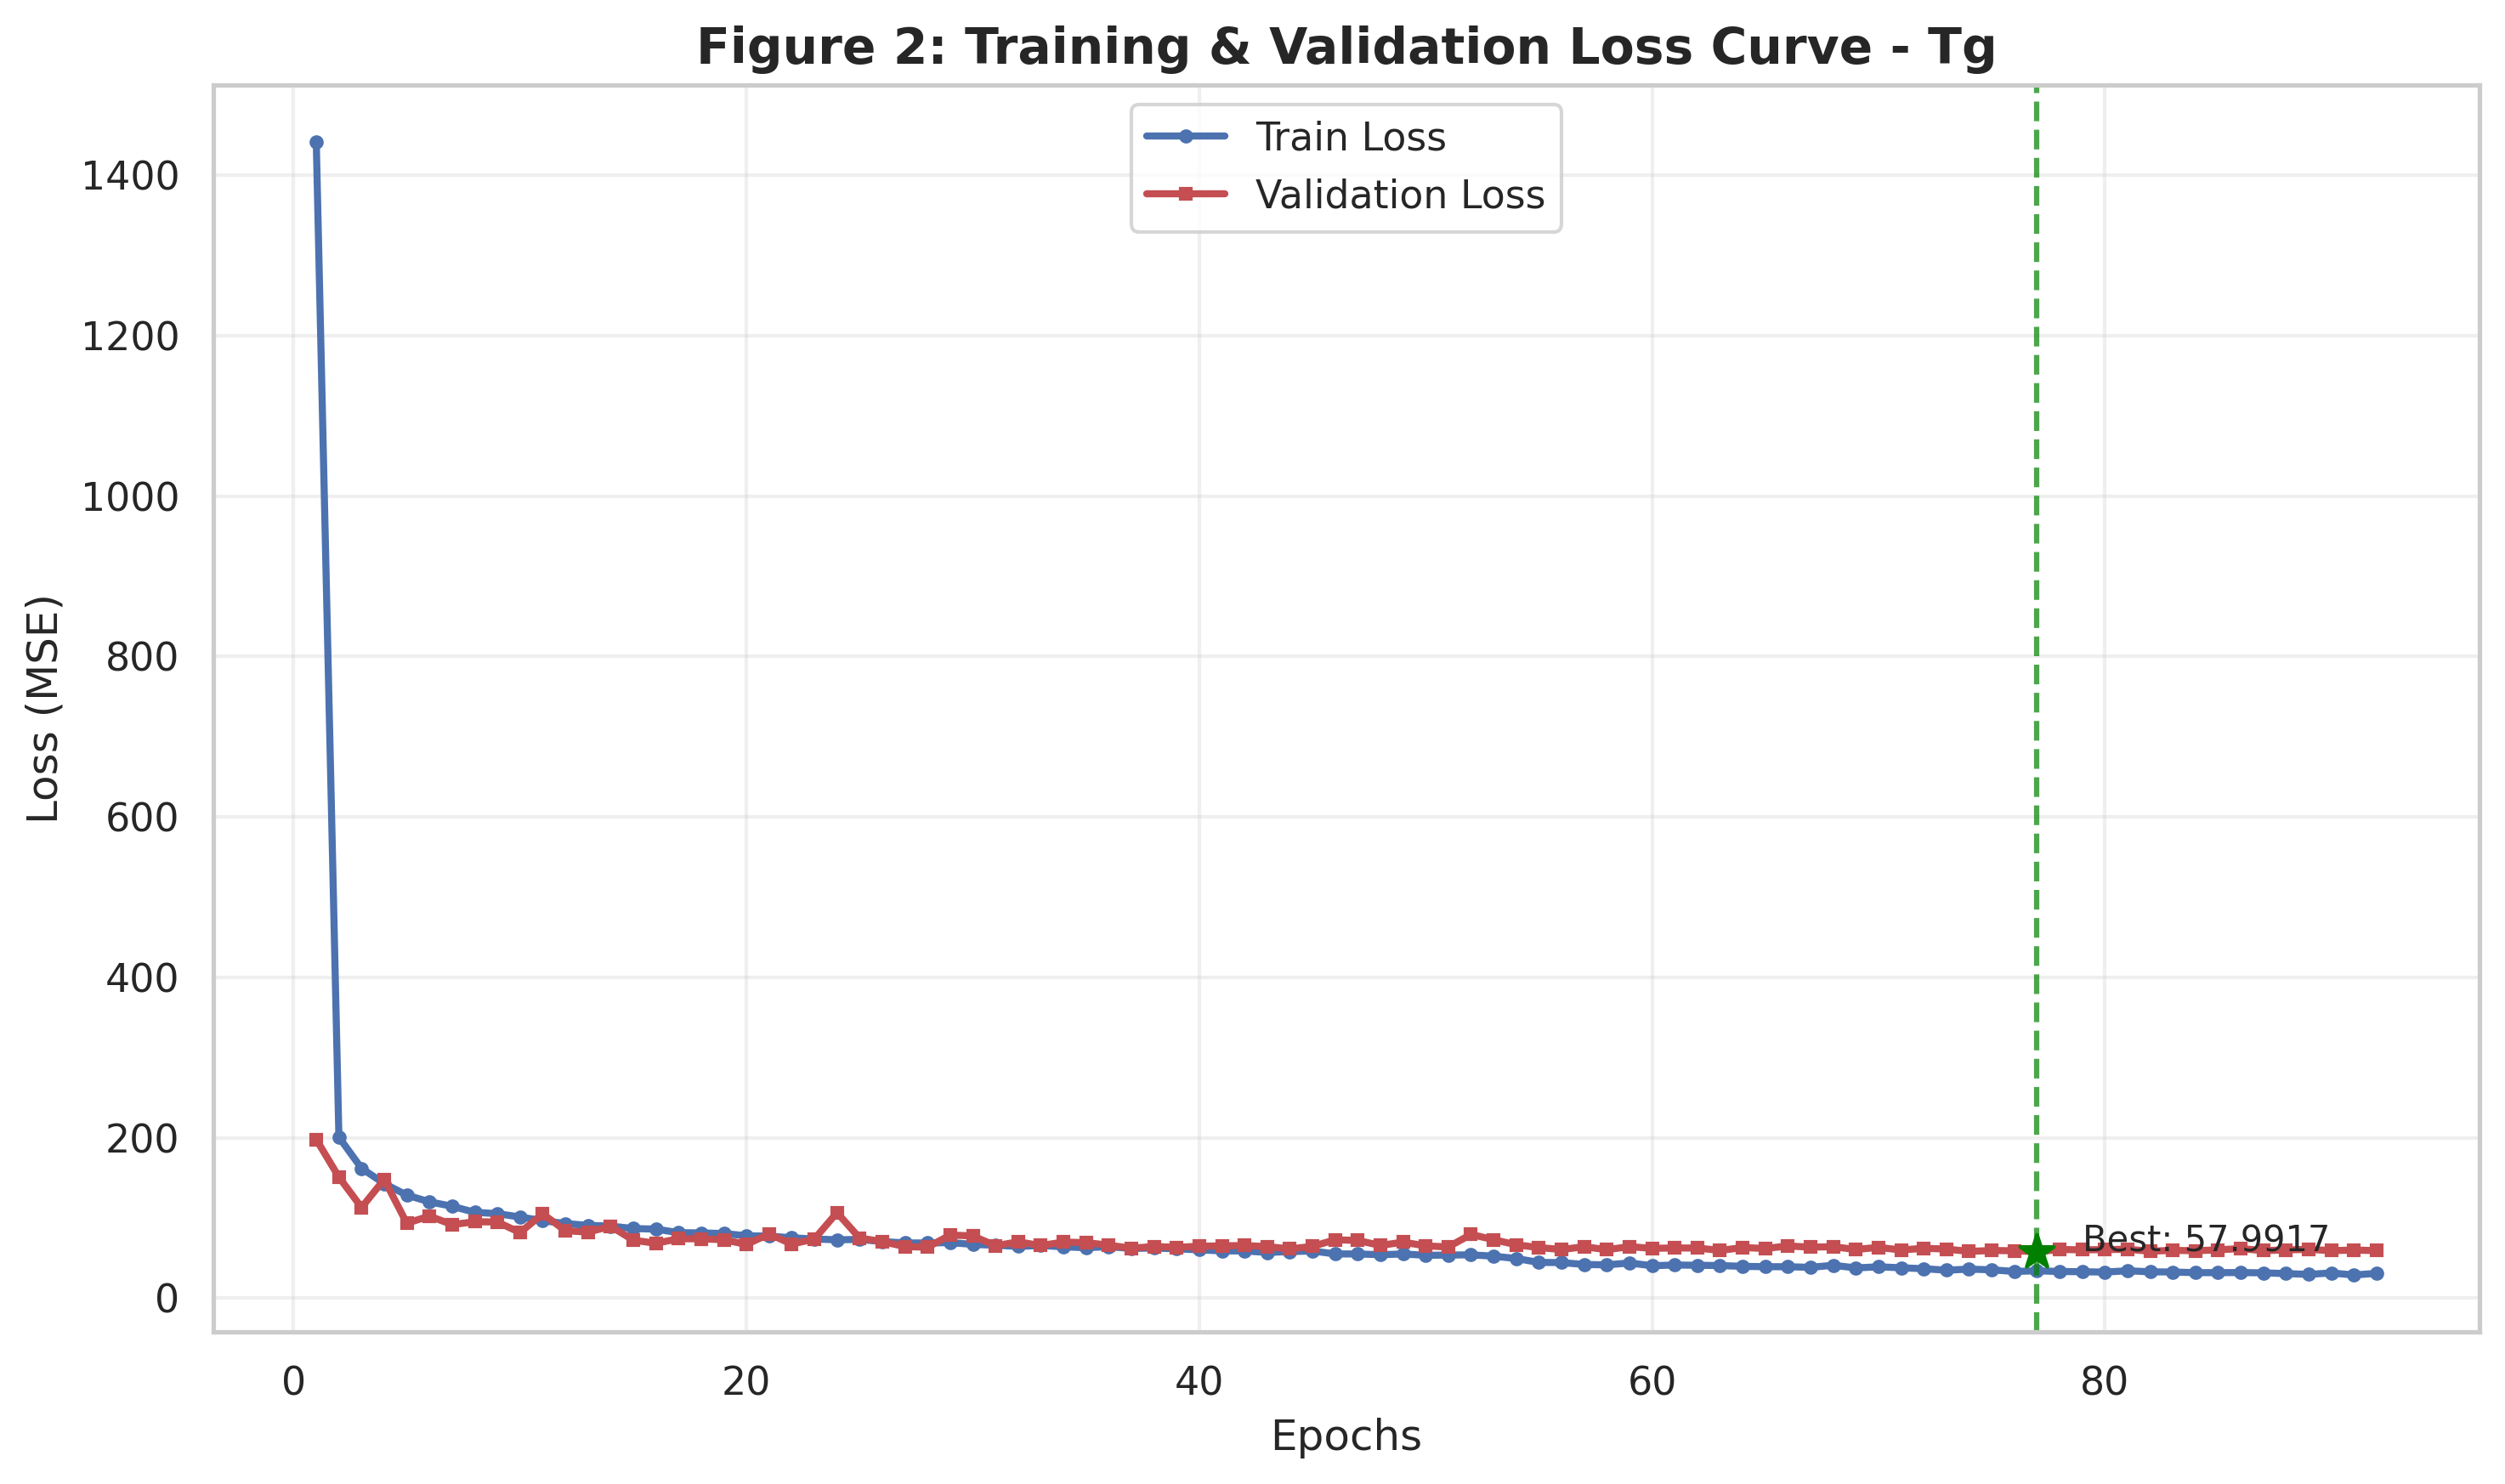
\includegraphics[width=\textwidth]{plots_Tg/fig2_loss_curve_Tg.png}
        \vspace{-1.5em}
        \caption{$T_g$}
        \label{fig:loss_tg}
    \end{subfigure}
    \hfill
    \begin{subfigure}[b]{0.32\textwidth}
        \centering
        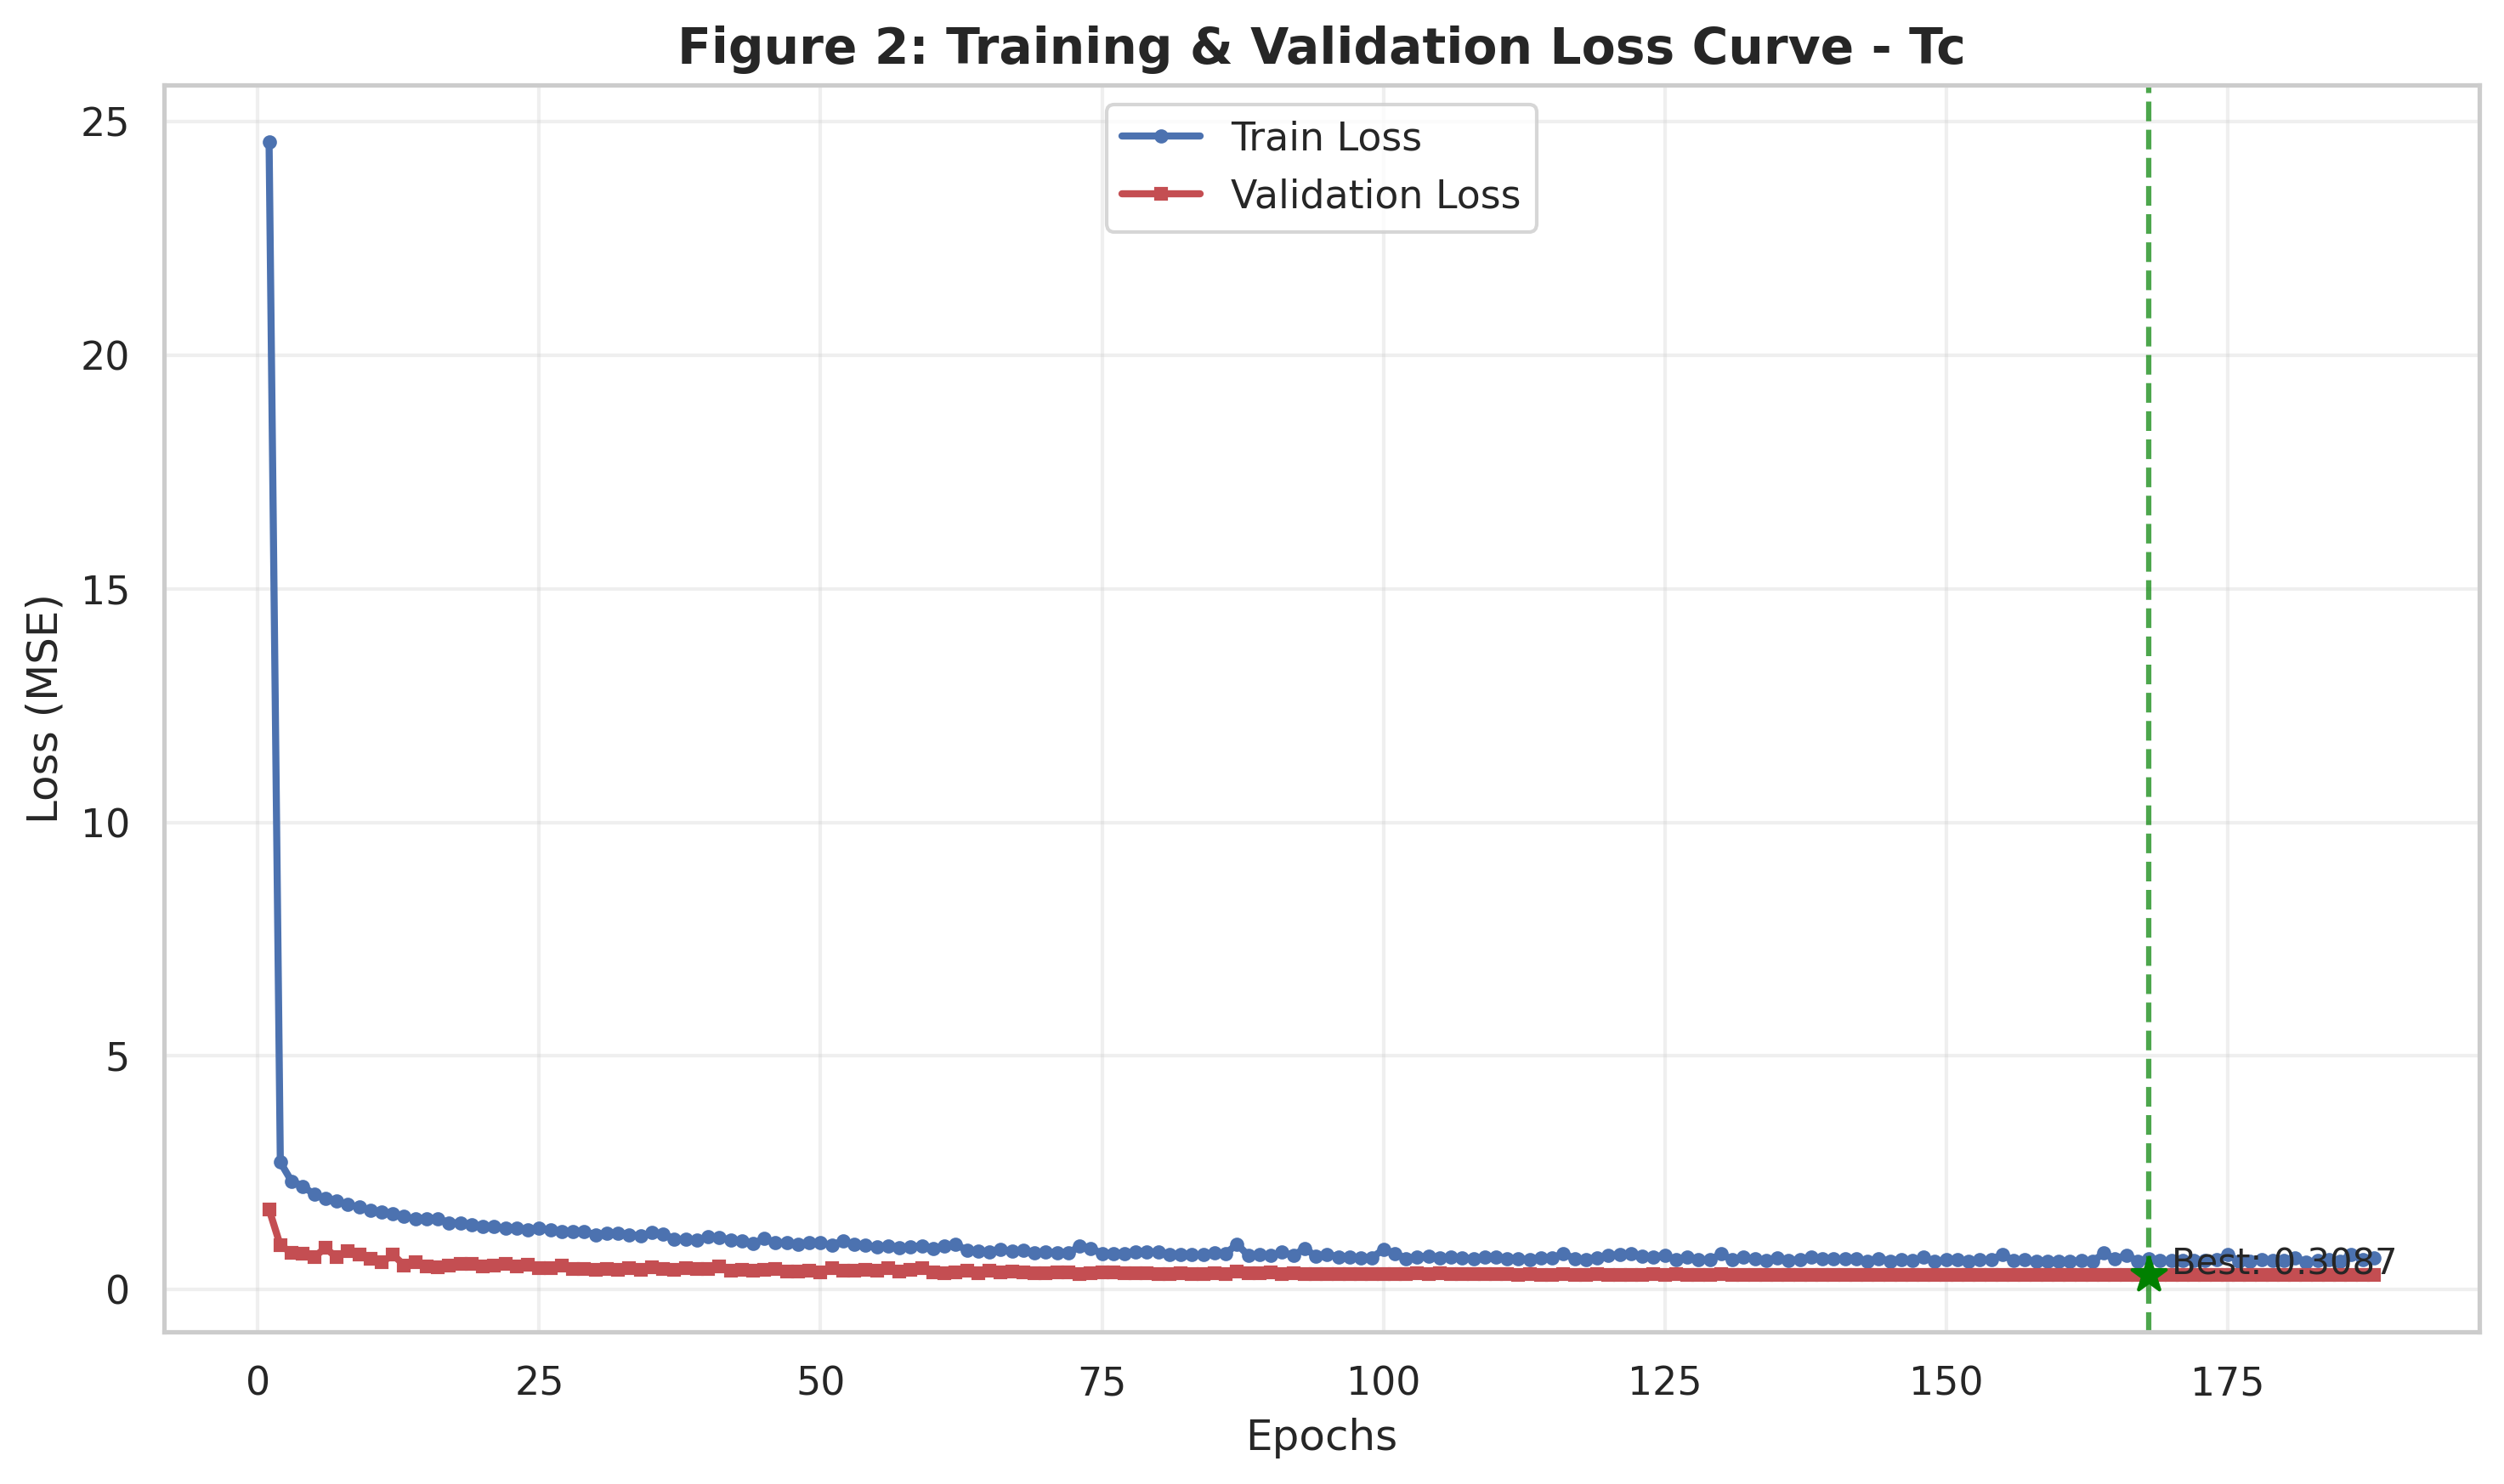
\includegraphics[width=\textwidth]{plots_Tc/fig2_loss_curve_Tc.png}
        \vspace{-1.5em}
        \caption{$T_c$}
        \label{fig:loss_tc}
    \end{subfigure}
    \hfill
    \begin{subfigure}[b]{0.32\textwidth}
        \centering
        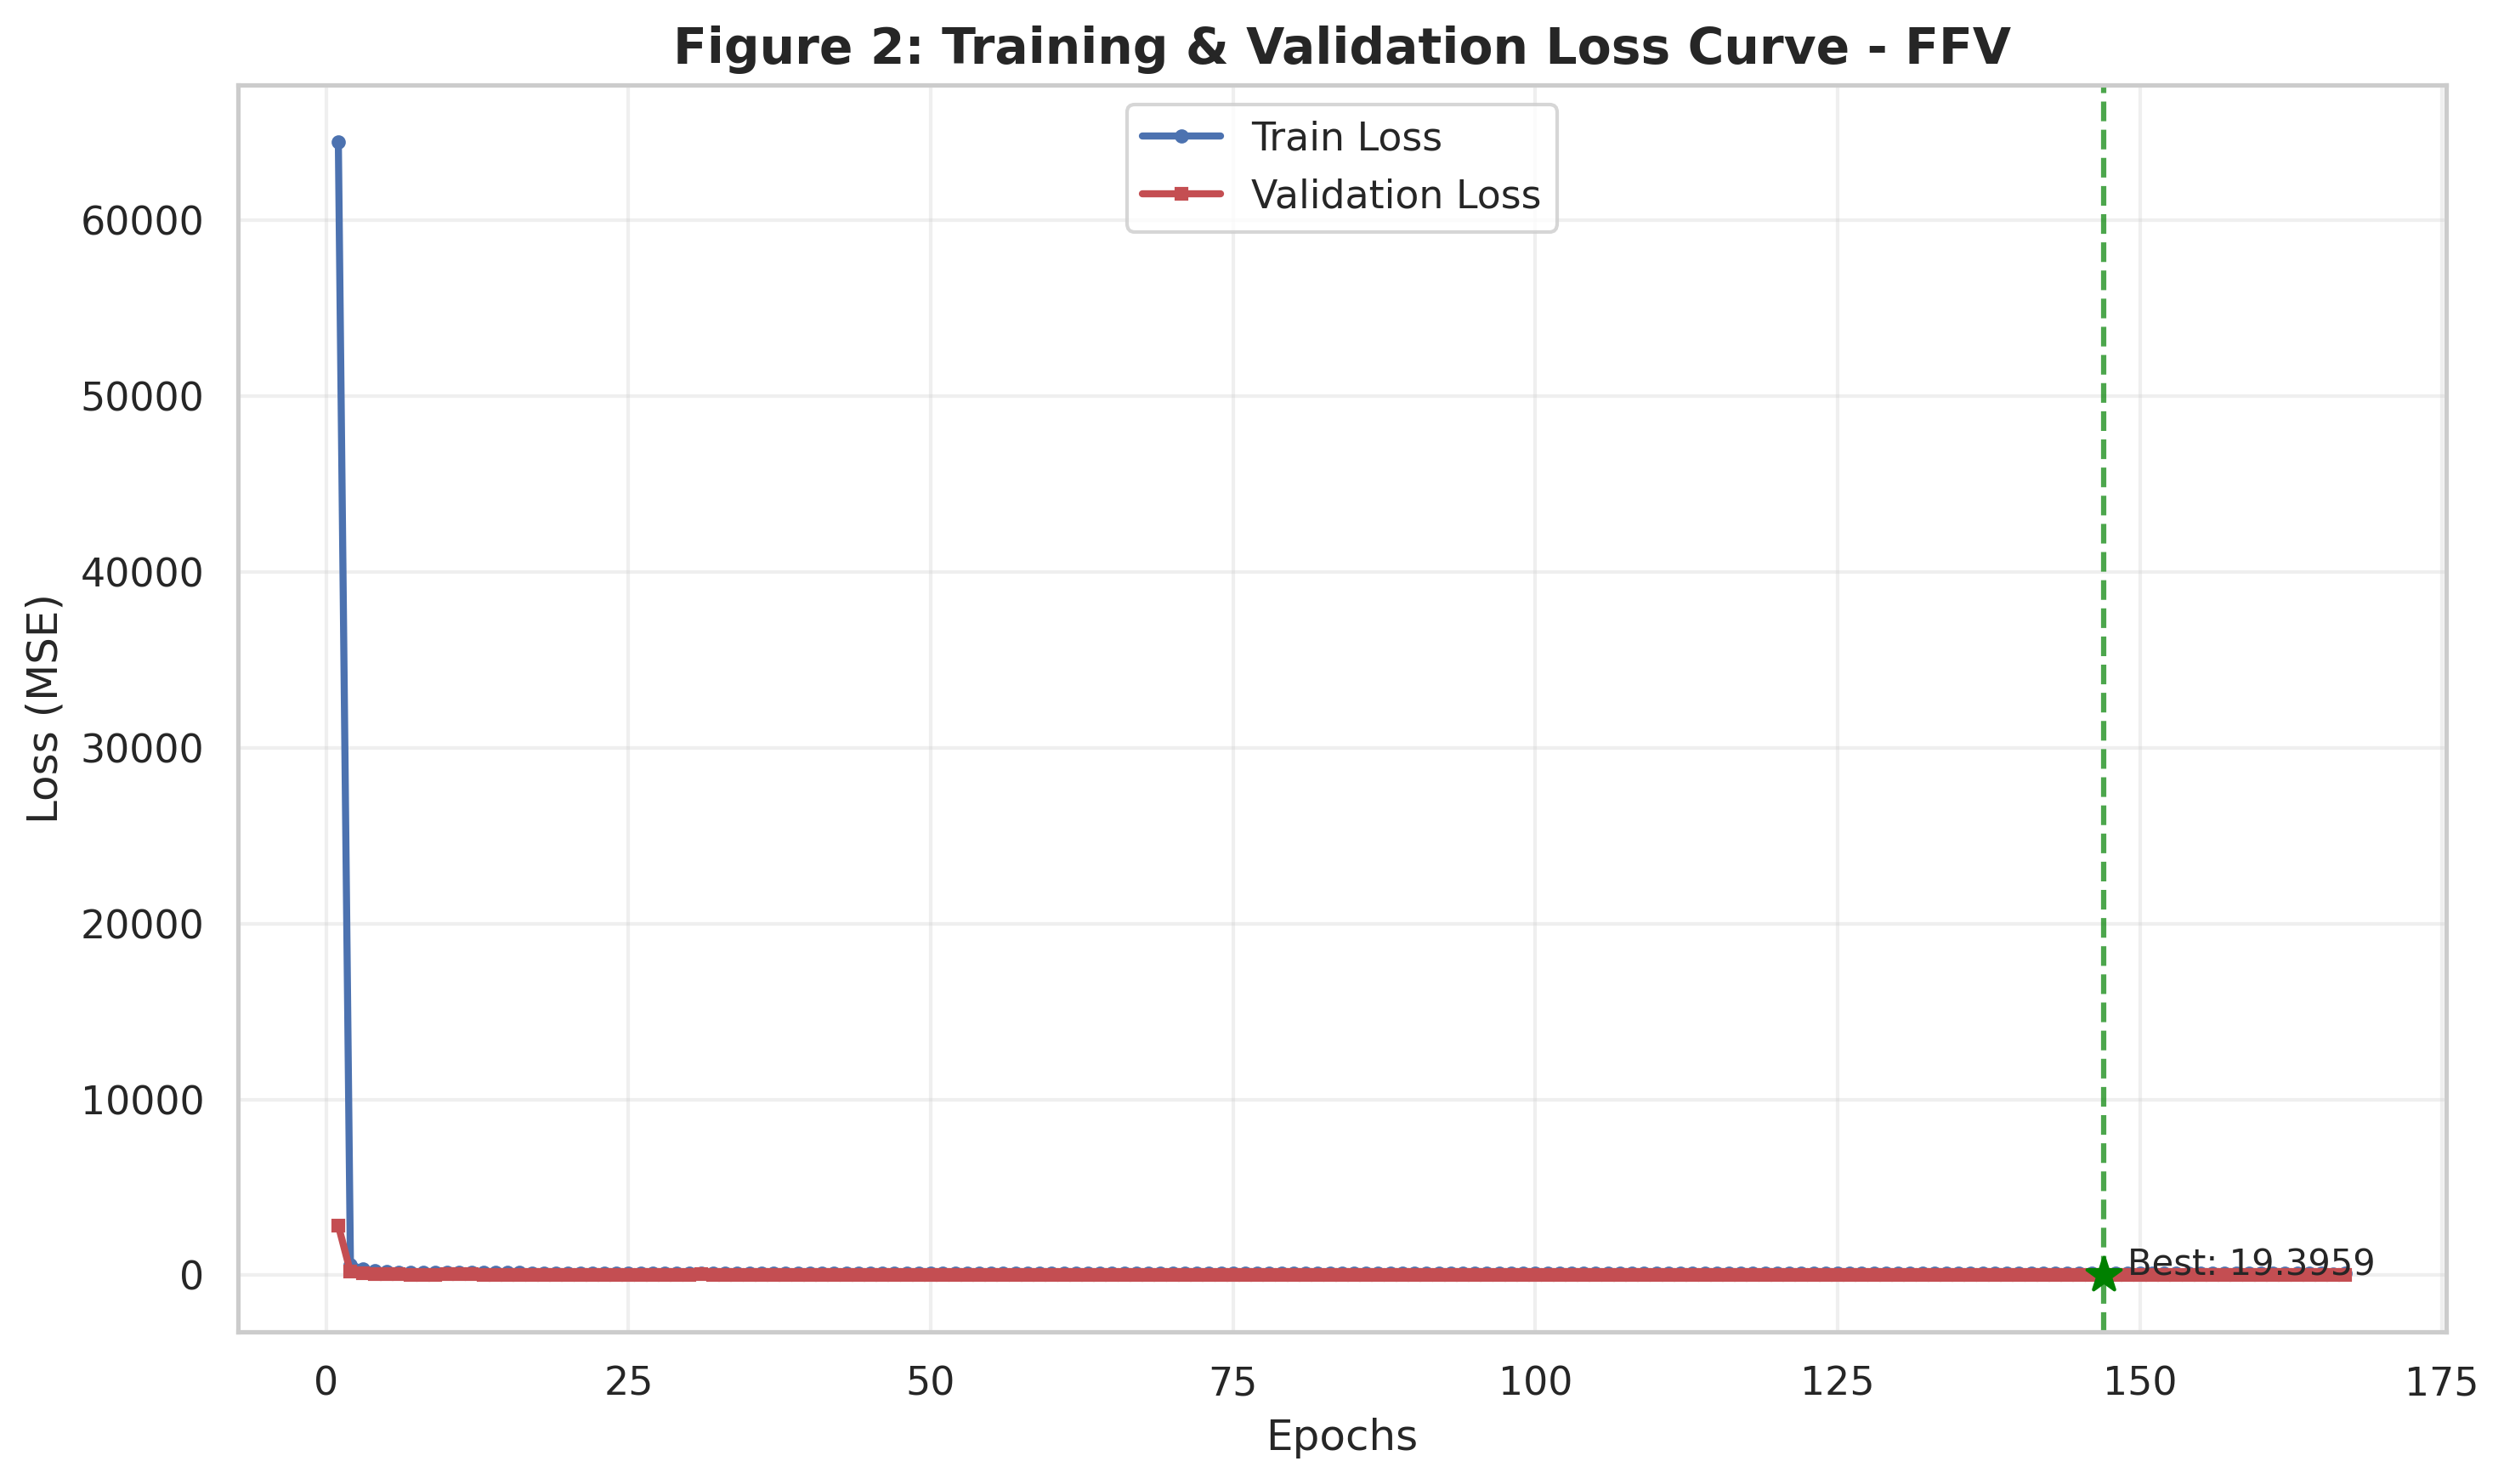
\includegraphics[width=\textwidth]{plots_FFV/fig2_loss_curve_FFV.png}
        \vspace{-1.5em}
        \caption{FFV}
        \label{fig:loss_ffv}
    \end{subfigure}

    \vspace{-0.5em}

    \begin{subfigure}[b]{0.32\textwidth}
        \centering
        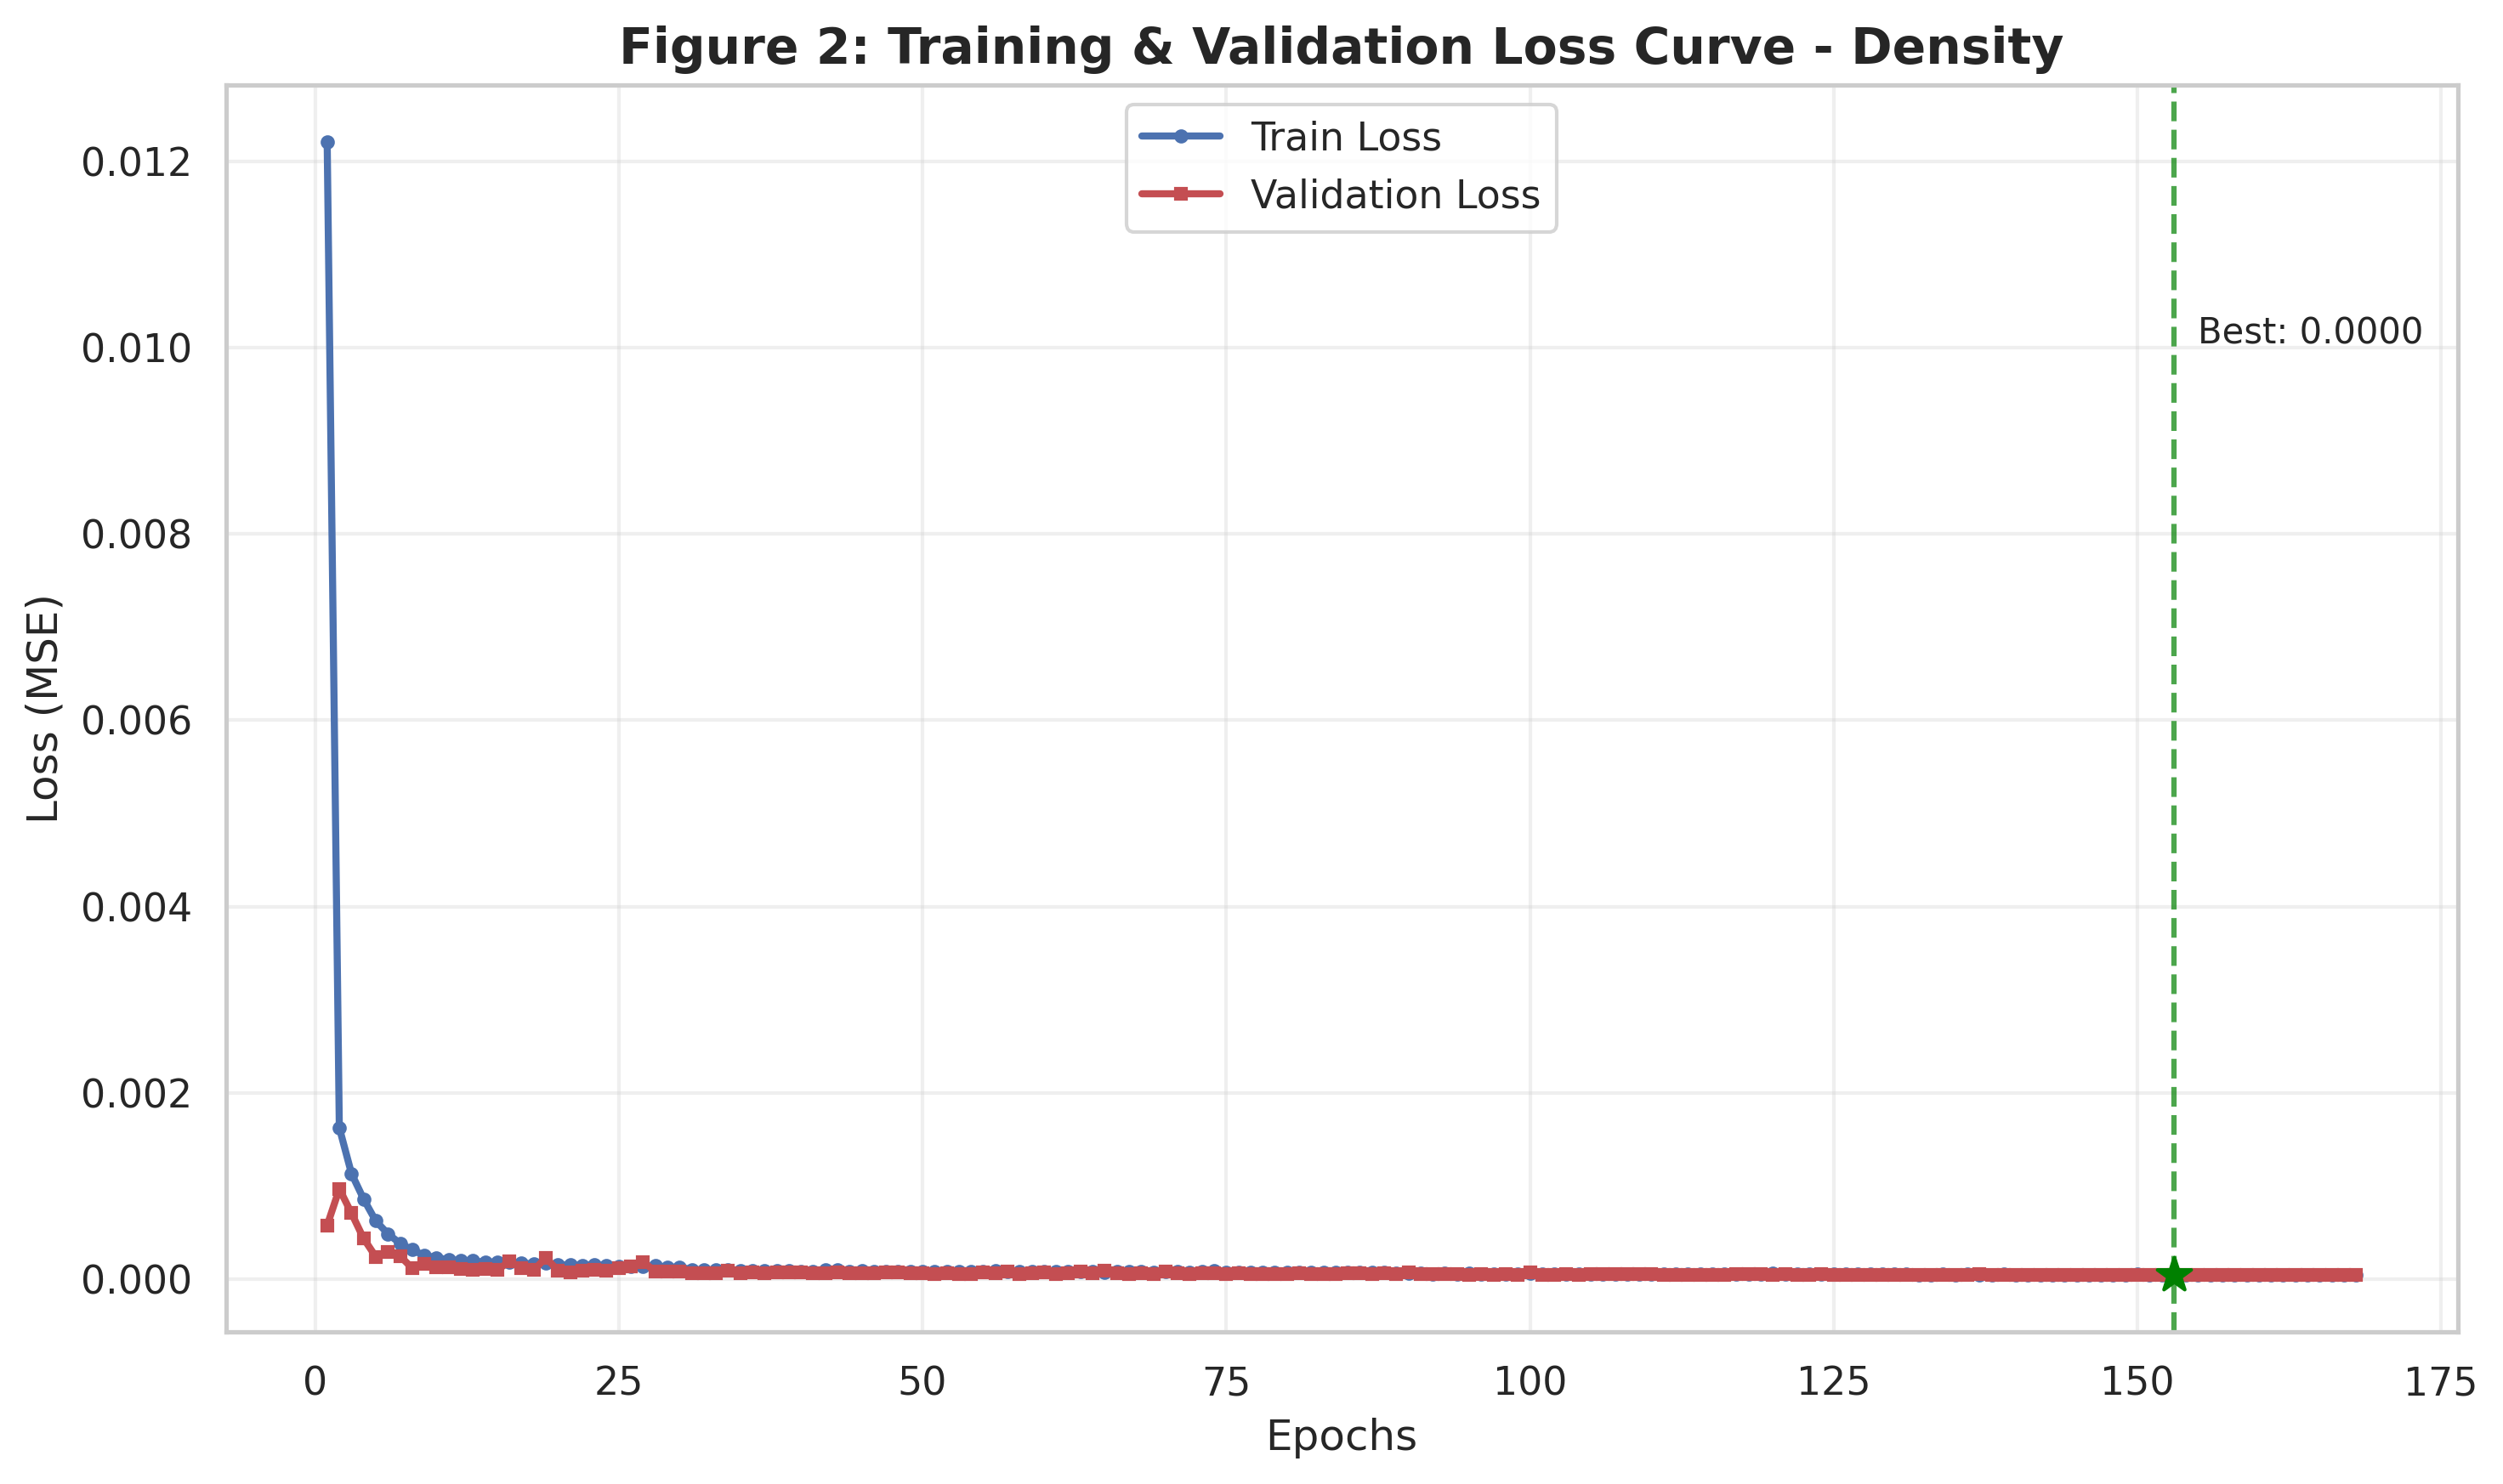
\includegraphics[width=\textwidth]{plots_Density/fig2_loss_curve_Density.png}
        \vspace{-1.5em}
        \caption{Density}
        \label{fig:loss_density}
    \end{subfigure}
    \hspace{0.05\textwidth}
    \begin{subfigure}[b]{0.32\textwidth}
        \centering
        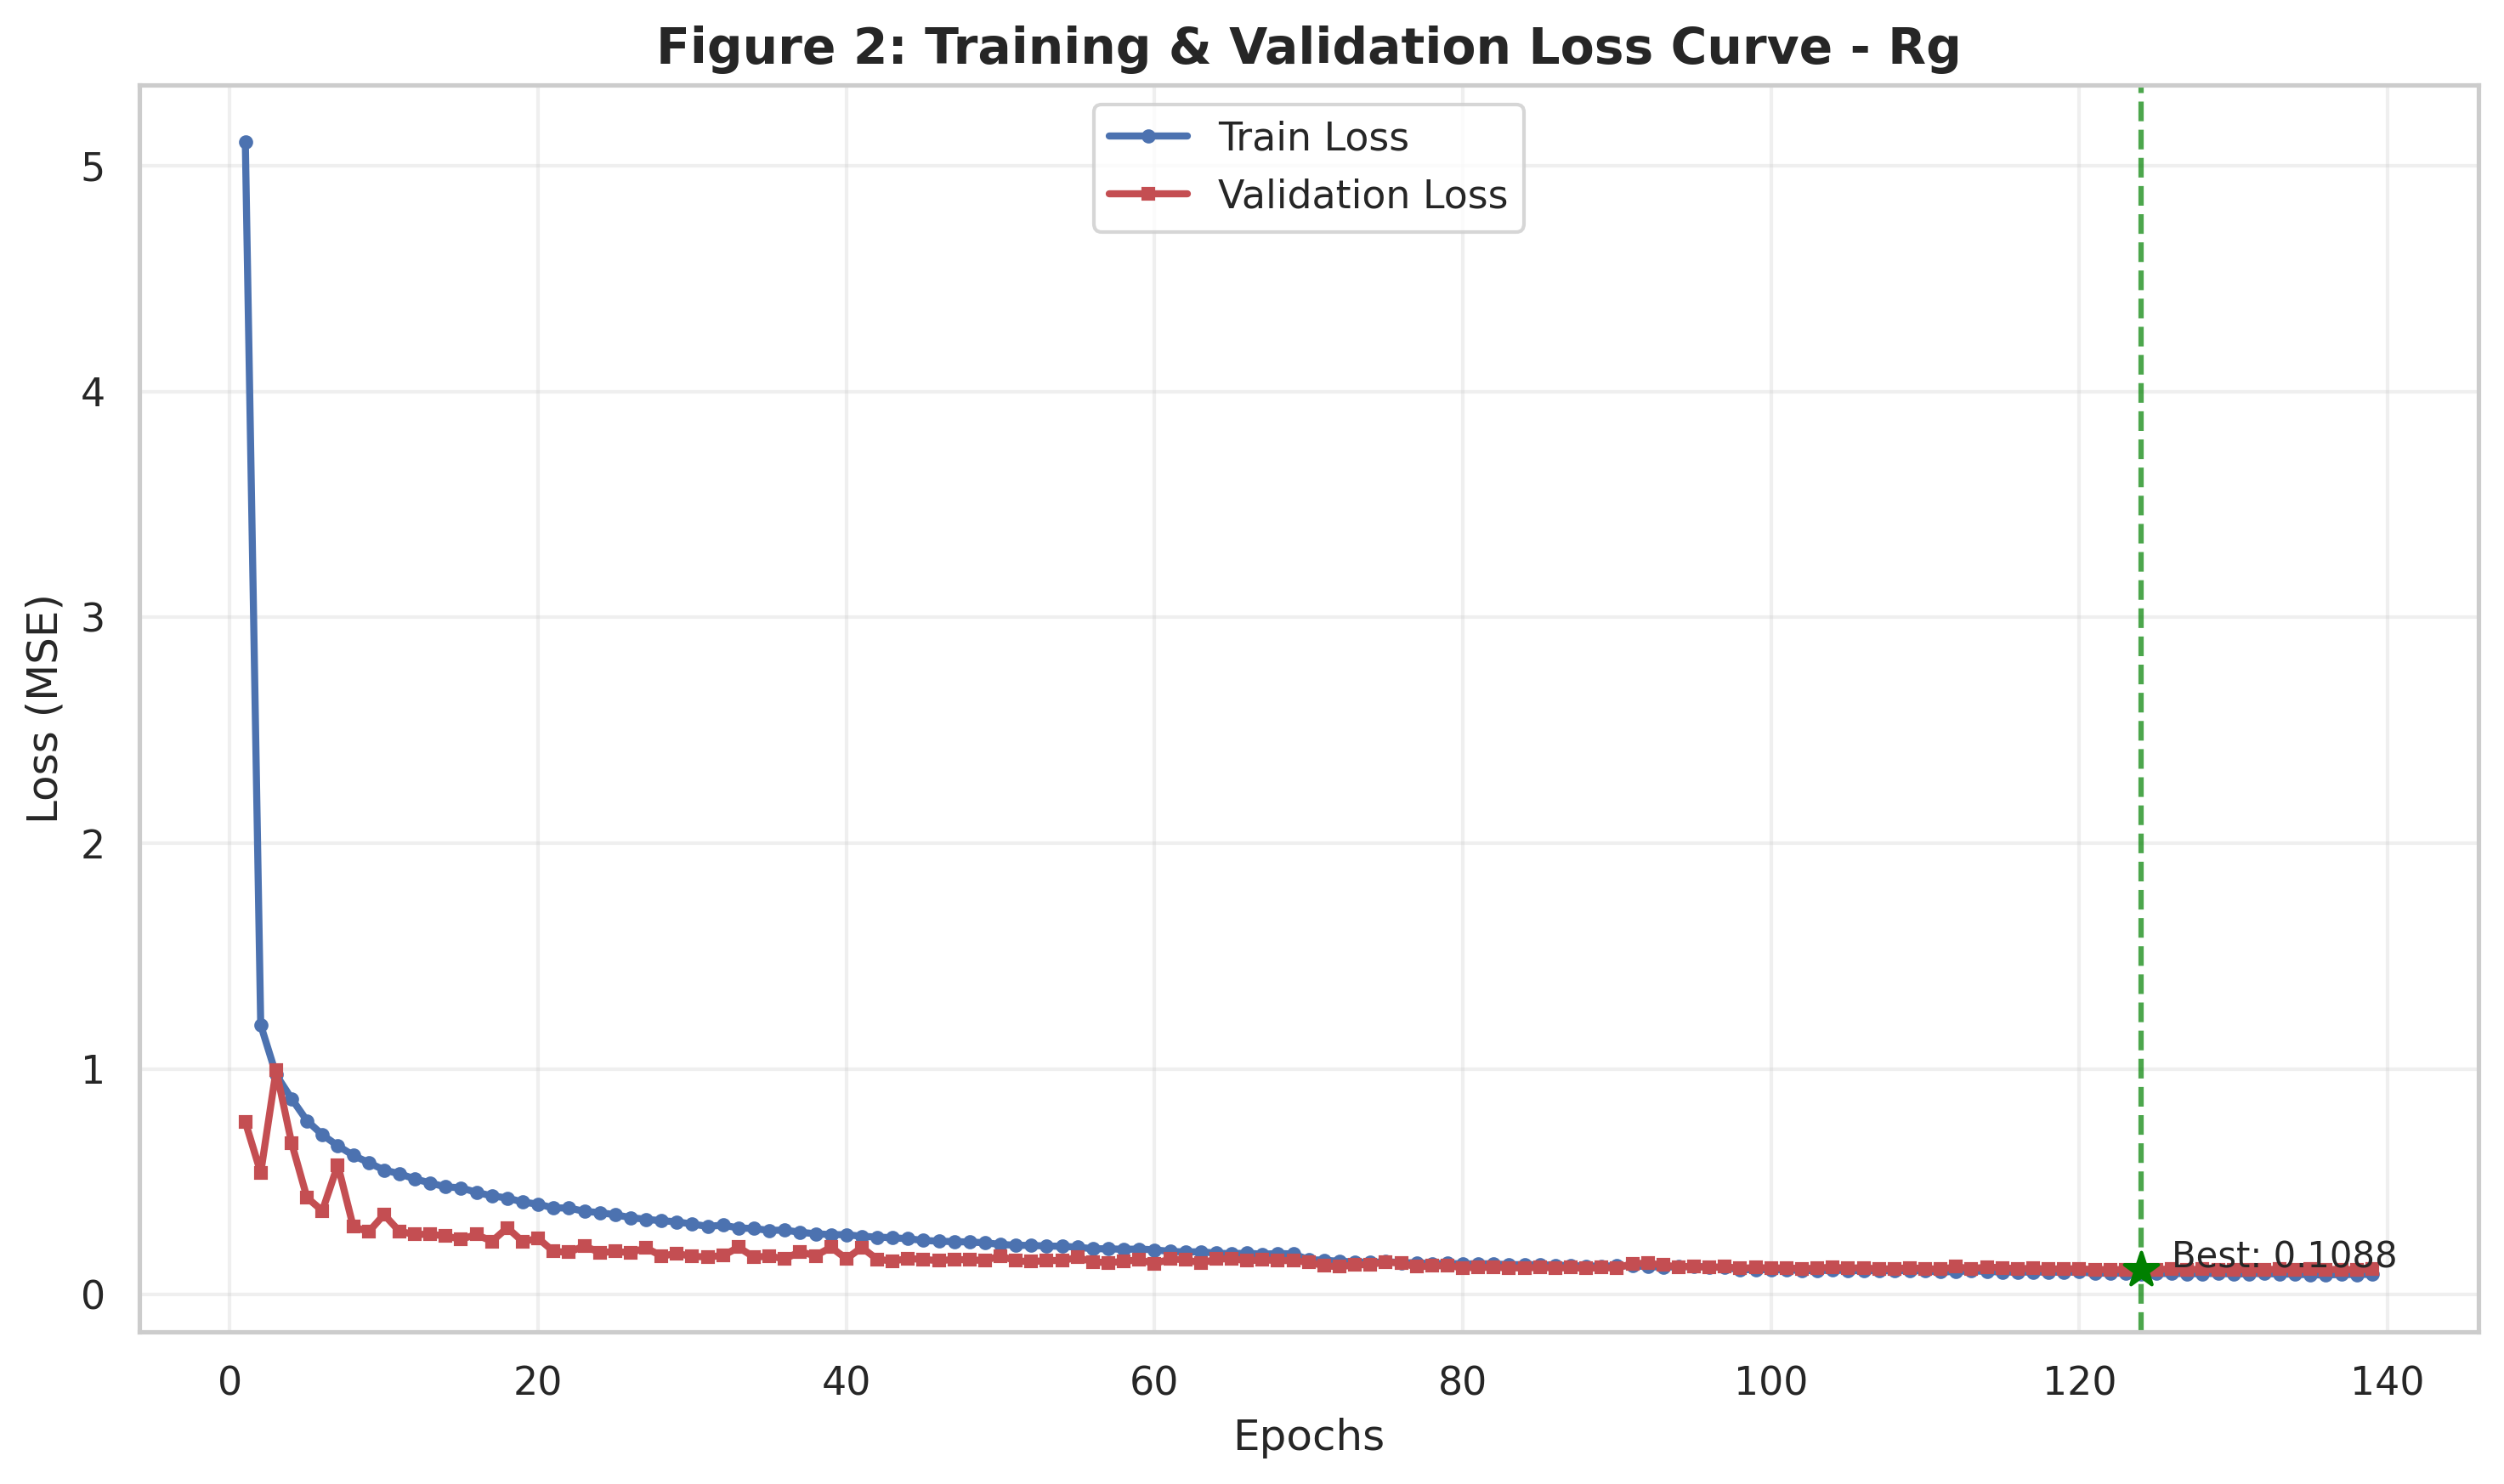
\includegraphics[width=\textwidth]{plots_Rg/fig2_loss_curve_Rg.png}
        \vspace{-1.5em}
        \caption{$R_g$}
        \label{fig:loss_rg}
    \end{subfigure}

    \caption{Epoch-selection stage for the full model under structure-grouped five-fold cross-validation. Thin lines: individual folds. Thick lines: fold mean of the standardised training loss (left axis, solid) and inner-validation MAE (right axis, dashed).}
    \label{fig:loss_curves}
\end{figure}

Two properties of the protocol matter for interpretation. First, epoch selection is performed on an inner split carved out of the outer training fold and grouped by structure, so the outer OOF predictions are never used for model selection; each outer test fold is scored exactly once. Second, the target standardisation and descriptor scaling used in a given stage are fitted only on the rows present in that stage. Consequently the OOF metrics in \Cref{tab:model_performance} are not optimistically biased by selection, although they remain conditional on this particular reconstruction of the benchmark data.

\subsection{Validation-domain limitation}

The primary split is structure-grouped: canonical repeat-unit SMILES with stereochemistry removed define the grouping key, and SMILES augmentation is applied only to training rows after the split. This prevents identical canonical structures and stereochemical variants from crossing folds. A broader equivalence analysis for reversed repeat-unit traversals, connection-point relabelling, periodic multiples and highly similar but distinct polymers was not completed in the verified analysis archive. Accordingly, the reported cross-validation estimates characterize interpolation within the reconstructed benchmark distribution; they should not be interpreted as evidence of extrapolation to novel chemical space. A similarity-clustered sensitivity analysis remains necessary before making an out-of-domain generalization claim.

\section{Discussion}

This study presents a hybrid deep learning framework combining sequence learning, frozen pretrained molecular embeddings, and explicit physicochemical descriptors to predict five macroscopic polymer properties from monomer SMILES strings. All results are based on structure-grouped cross-validation of the merged benchmark, with baselines retrained under the same protocol for direct comparison.

\subsection{Interpolation, Extrapolation, and the Value of Grouped Validation}

The most important methodological conclusion concerns validation design, not architecture. SMILES strings are non-unique: the same repeat unit can be written in many equivalent ways, and augmented enumerations multiply the number of strings per structure. A random split over strings therefore places identical chemistry in both training and validation sets and produces optimistically biased estimates. Grouping structures before splitting, augmenting only after the split and only within training folds, and fitting scalers on training rows only are each necessary; omitting any one of them invalidates the estimate.

Even so, the present protocol controls only structural identity up to stereochemistry: group identifiers are computed from canonical SMILES with stereochemical information removed, so stereochemical variants of one structure always share a group, but no broader equivalence is enforced. Repeat-unit representations that differ by connection-point placement, traversal direction, or periodic multiple remain separate groups unless they canonicalize identically. We have not established equivalence under all such transformations. The results in \Cref{tab:model_performance} should therefore be read as performance on held-out structures drawn from the same chemical distribution as the training set---that is, as interpolation---rather than as evidence of extrapolation to novel chemical space.

\subsection{Complementary but Non-Uniform Roles of the Feature Modalities}

The ablation study does not support the intuitive picture in which every module helps every property. Under the reported fold assignment no target is numerically best predicted by the full model: the CNN-removed variant is numerically best for $T_g$, FFV, density and $R_g$, and the augmentation-removed variant for $T_c$; no difference survives Holm correction across the 30 comparisons.

Several explanations remain compatible with the numerical pattern. Reduced models have numerically lower MAE for every target, so a small-sample explanation cannot cover the pattern: the CNN-removed variant is also numerically best for FFV, which has 7{,}892 labels. Feature redundancy is another hypothesis, but the non-significant comparisons do not distinguish it from training or split variability for any target. Repeated training runs, controlled feature-overlap analyses or sample-size scaling studies would be needed to evaluate these explanations.

The numerical increase in $R_g$ MAE after removing the backbone/sidechain descriptors ($+0.228$\,\AA) is compatible with the physical role of chain topology in chain dimensions. This comparison is not statistically significant after multiplicity correction, however, so its physical plausibility does not establish a reliable descriptor benefit.

\subsection{Pretrained Embeddings and Domain Mismatch}

MolFormer was pretrained primarily on small-molecule SMILES, whereas the present inputs are polymer repeat units. In the verified ablation, removing the frozen embedding changes the five MAEs in different directions: it increases $T_g$, $T_c$ and $R_g$ errors but decreases FFV and density error. None of these paired comparisons is statistically significant after correction for the 30 ablation comparisons. The data therefore do not establish a uniform MolFormer benefit, nor do they demonstrate that the representation is unsuitable for polymers. Polymer-specific controls such as PolyNC and polyBERT were not available in the verified same-protocol archive and are not reported as quantitative baselines; their evaluation remains future work.

\subsection{Limitations}
\label{sec:limitations}

Several limitations of the current work should be acknowledged.

\textbf{Dataset scope and label heterogeneity.} Our evaluation is confined to the NeurIPS 2025 challenge dataset, and the five targets are very unevenly labelled ($T_g$, $T_c$, $\rho$ and $R_g$ each have fewer than 900 labelled structures, versus 7{,}892 for FFV). The labels originate from molecular-dynamics simulations whose settings are not fully documented per record. Two cross-source label conflicts were detected and resolved by retaining the primary value; other unobserved heterogeneity in simulation conditions may remain. Generalization to other polymer datasets with different chemical spaces or property ranges is unvalidated.

\textbf{Repeat-unit representation and chain-length dependence.} The model operates on monomer SMILES strings representing idealized repeating units. These contain no molecular weight, degree of polymerization, or molecular-weight distribution. Chain-size effects may limit transfer to polymers constructed at other degrees of polymerization, but their contribution to the present benchmark error has not been measured. The $R_g$ construction protocol and the limits of its verification against the training records are discussed below. Other variables absent from the input include tacticity, crosslink density, copolymer sequence, end groups, crystallinity, chain entanglement, chain conformation, interchain packing, free-volume distribution and defects; their omission identifies possible limitations without establishing an error floor.

\textbf{Simulation conditions and transfer to experiments.} Temperature, pressure, cooling schedule, equilibration history, simulation box size and force field are absent from the model input. These conditions define the simulated target values, and differences between protocols could affect transfer to other simulation datasets. Their contribution to error within this benchmark has not been quantified. Application to experimental measurements additionally requires validation against experimental data with documented measurement and processing conditions.

\textbf{Absence of 3D information.} SMILES representations do not encode three-dimensional conformational information. While the backbone/sidechain descriptors partially address topological features, properties influenced by specific 3D conformations (e.g.\ crystallinity, mechanical properties) cannot be accurately predicted from 1D representations alone.

\textbf{Descriptor implementation.} Eleven of the 17 declared fields are initialized to zero and never computed in the inference-derived function used for re-analysis. This is an implementation defect relative to a claimed 17-feature descriptor block, not a chemical characteristic of the data. Additionally, 18 structures do not have exactly two wildcard atoms and receive an all-zero descriptor vector. Existing scores evaluate this limited implementation; they do not quantify the value of the omitted features.

\textbf{Structural equivalence and grouping.} The group identity used for cross-validation is the canonical SMILES with stereochemical information removed, so stereoisomers are assigned to the same group. Repeat-unit shifts, reversed traversal, alternative connection-point labels and different periodic multiples are not guaranteed to map to the same group. Residual leakage through such equivalences cannot be excluded.

\textbf{Validation protocol.} The primary results rest on one seed and one family of grouped folds; training stochasticity is not separately controlled. Prediction intervals were not computed; the bootstrap intervals in \Cref{tab:model_performance} quantify uncertainty of the error estimate, not of individual predictions.

\textbf{Baseline coverage.} The verified same-protocol baselines are the mean predictor, Morgan--Ridge, Morgan--random forest, a transferred Chen recurrent model and an adapted PU-GN model. Their results are kept separate from literature values because the adaptations and model-selection budgets are not identical. PolyNC and polyBERT were not run in the verified archive; no numerical performance claim is made for them.

\textbf{Domain of applicability.} The current framework predicts dataset-conditioned property values from repeat-unit chemistry under the assumptions and conditions represented in the benchmark. It does not explicitly account for molecular weight, morphology, processing history, or experimental conditions, and is more appropriate for relative screening within a chemical domain similar to the training set than for direct prediction of arbitrary bulk-polymer properties under uncontrolled conditions.

\textbf{Property-specific physical limitations.} The five targets depend on physical variables and simulation protocols that are not fully represented by repeat-unit SMILES. The following considerations describe potential limitations of the representation and of transfer beyond the benchmark; they do not establish an irreducible MAE for this dataset:

\emph{Glass transition temperature ($T_g$)}: Simulated $T_g$ can depend on chain size, cooling schedule, equilibration history and the procedure used to extract the transition from the simulated trajectory. Repeat-unit chemistry alone does not specify these variables. Differences between experimental methods such as DSC and DMA would require separate validation when applying the model to experimental data; they do not establish an error floor for the MD labels evaluated here.

\emph{Fractional free volume (FFV)}: Free volume depends on interchain packing, temperature, pressure and the geometric definition used in its calculation. Force-field choice, equilibration and conformational sampling can affect the simulated structures from which FFV is obtained. The model learns the benchmark's FFV labels from repeat-unit features; transfer to other packing states or calculation protocols has not been validated.

\emph{Thermal conductivity ($T_c$)}: Heat transport depends on chain conformation and alignment, interchain contacts, morphology and the simulation protocol used to estimate conductivity. These variables are not explicitly provided to the model. Performance on this benchmark therefore does not establish accuracy for polymers with different morphology or for conductivity obtained under different simulation or experimental protocols.

\emph{Density ($\rho$)}: Density depends on temperature, pressure, morphology and interchain packing, while the simulated value can also depend on equilibration and force-field choices. The model predicts density under the conditions represented by the benchmark; transfer to other thermodynamic states or processed experimental samples requires independent validation.

\emph{Radius of gyration ($R_g$)}: Chain dimensions depend on degree of polymerization, chain stiffness, thermodynamic state and conformational sampling. The organizers' post-competition report describes an amorphous-cell protocol with approximately 600 atoms per chain and six chains per cell, with $R_g$ averaged over time and chains at 300\,K and 1\,atm.\cite{liu_open_polymer_report_2025} A target atom count is not a fixed degree of polymerization: the number of repeat units needed depends on repeat-unit size. The released training records used here do not include chain size or degree of polymerization, so we have not verified this construction rule for each training label. Our predictions are therefore interpreted as benchmark-conditioned chain dimensions; extrapolation to other chain sizes has not been validated.

No repeated-simulation analysis or dataset-specific estimate of conditional label variability was performed in this study. Missing inputs alone do not quantify an irreducible MAE. The reported cross-validation errors combine the effects of model approximation, finite training data and any label variability; the present analysis does not separate these contributions. We therefore make no claim that any property approaches a physical accuracy limit or lies a specified factor above a noise floor.

\subsection{Future Directions}

Several extensions could address the limitations identified above.

\textbf{3D structural information.} Incorporating geometric features from 3D molecular graphs or brief molecular dynamics simulations could improve prediction of conformation-dependent properties. Graph neural networks operating on 3D atomic coordinates represent a promising direction.

\textbf{Molecular weight dependence.} Feeding molecular weight parameters (e.g., number-average or weight-average molecular weight) as explicit inputs could improve prediction of properties sensitive to chain length, such as $R_g$ and $T_g$.

\textbf{Polymer-specific pretraining and fine-tuning.} Evaluating PolyNC and polyBERT under the same folds, labels and metrics, followed by controlled fine-tuning, would directly address the domain mismatch question.

\textbf{Applicability domain.} A similarity-clustered split and a per-prediction applicability-domain measure remain open requirements for testing extrapolation.

\textbf{Inverse design.} The current framework focuses on forward prediction (structure to property). Integrating the learned representations with generative models could enable inverse design---identifying polymer structures that satisfy target property specifications.

\section{Conclusion}
\label{sec:conclusion}

Poly-Prophet combines repeat-unit sequence features, frozen MolFormer embeddings and backbone/sidechain descriptors in five independently trained property-specific regressors. Under the verified structure-grouped five-fold protocol, fold-mean MAEs are \(53.44 \pm 4.79\)\,K for \(T_g\), \(0.00507 \pm 0.00031\) for FFV, \(0.03108 \pm 0.00291\)\,W\,m\(^{-1}\)\,K\(^{-1}\) for \(T_c\), \(0.02835 \pm 0.00376\)\,g\,cm\(^{-3}\) for density, and \(1.402 \pm 0.144\)\,\AA for \(R_g\). The verified same-protocol baselines show lower numerical error for the transferred Chen model on \(T_g\), while the full model is lower for FFV, \(T_c\), density and \(R_g\); these are descriptive comparisons on one reconstructed benchmark and do not establish universal superiority. Ablation directions are property-dependent and none of the 30 corrected comparisons is statistically significant. The original 4.02 K and 0.225 \AA values are excluded because their data and protocol cannot be traced. The model should therefore be treated as a reproducible benchmark baseline for interpolation within this chemical domain; transfer to new chemical spaces, experimental conditions or polymers whose molecular weight, morphology and processing history differ requires independent validation.

\section{Methodology}

We present a hybrid deep learning framework for predicting five macroscopic polymer properties from repeat-unit SMILES strings. Each property is predicted by a separate, independently trained regressor; the five regressors share the architecture and training protocol described below and are not connected by a shared output layer or a joint loss. The data processing pipeline, validation design and model architecture are described in the following sections.

\subsection{Dataset and Target Properties}

The primary dataset is derived from the NeurIPS 2025 Open Polymer Prediction Challenge.\cite{neurips-open-polymer-prediction-2025} It comprises polymer repeat-unit SMILES strings paired with five target properties obtained via molecular dynamics (MD) simulations: glass transition temperature ($T_g$), thermal conductivity ($T_c$), fractional free volume (FFV), density ($\rho$), and radius of gyration ($R_g$). Absolute $T_g$ labels follow the competition documentation and are expressed in $^\circ$C; error metrics for $T_g$ are expressed in K, which is numerically identical for temperature differences.

The organizers' post-competition report provides simulation-generation details, including an approximately 600-atom-per-chain construction protocol for density, $R_g$ and $T_c$ and time- and chain-averaging of $R_g$.\cite{liu_open_polymer_report_2025} The released training table used here contains repeat-unit structures and target values, but no per-record chain-size or degree-of-polymerization annotation. We therefore distinguish the reported generation protocol from a verified assignment of simulation settings to every training record; neither a fixed degree of polymerization nor undocumented random chain-length variation is assumed in interpreting our results.

Three labelled supplementary sources (targeting $T_c$, $T_g$ and FFV) and one unlabelled source were provided by the competition organizers. The rebuilt merged set contains 8{,}972 unique canonical repeat-unit structures, distributed across the sources as 7{,}973 (primary), 866 ($T_c$ supplement), 46 ($T_g$ supplement), 862 (FFV supplement), and 7{,}174 unique unlabelled structures. Label counts after merging are 557 ($T_g$), 7{,}892 (FFV), 866 ($T_c$), 613 ($\rho$) and 614 ($R_g$); \Cref{tab:dataset_composition} reports ranges, means and missingness. The unlabelled source is excluded from training and from all statistics.

\subsection{Dataset Integration and Duplicate Resolution}

Raw strings were checked for R-group placeholders and parsed with RDKit; no rows in the downloaded sources failed these checks (\Cref{tab:source_audit}). Wildcard connection atoms (*) were retained. Structures were standardized to canonical isomeric SMILES for source-level identity and duplicate resolution. Supplementary duplicate rows were averaged within each source; primary labels were preserved, while supplements filled missing labels or appended structures. The 737 primary/Dataset 1 and 38 Dataset 1/Dataset 4 overlaps were audited separately. Two cross-source label conflicts exceeding rtol $=10^{-6}$ and atol $=10^{-8}$ were resolved in favour of primary labels. All 8{,}972 final structures have at least one observed target; unlabelled Dataset 2 and visible-test structures are excluded. Cross-validation grouping subsequently removes stereochemistry and is distinct from the isomeric identity used for this audit.
\begin{table}[H]
\centering
\caption{Source-level cleaning and integration audit. Counts refer to rows and canonical isomeric repeat-unit structures, before cross-validation grouping.}
\label{tab:source_audit}
\scriptsize
\setlength{\tabcolsep}{3pt}
\begin{tabular}{lrrrrrrr}
\toprule
Source & Raw & Parse & R-group & Duplicate & Unique & Overlap & Added \\
 & rows & excluded & excluded & rows & structures & with merge & to training \\
\midrule
Primary train & 7,973 & 0 & 0 & 0 & 7,973 & --- & 7,973 \\
Dataset 1 ($T_c$) & 874 & 0 & 0 & 8 & 866 & 737 & 129 \\
Dataset 3 ($T_g$) & 46 & 0 & 0 & 0 & 46 & 0 & 46 \\
Dataset 4 (FFV) & 862 & 0 & 0 & 0 & 862 & 38 & 824 \\
Dataset 2 (unlabelled) & 7,208 & 0 & 0 & 34 & 7,174 & 5,803 & 0 \\
Visible test (unlabelled) & 3 & 0 & 0 & 0 & 3 & 3 & 0 \\
\bottomrule
\end{tabular}

\vspace{0.5em}
\footnotesize
Duplicate rows = valid rows minus unique canonical structures within a source. The labelled merge order is primary, Dataset 1, Dataset 3, Dataset 4, yielding 7,973, 8,102, 8,148 and 8,972 structures. Overlap is with the accumulated labelled merge at that step; the unlabelled sources are compared with the final merge but excluded from training. Dataset 2 has 1,371 structures outside that merge. Dataset 4's 38 overlaps are with Dataset 1, not the primary source; all 862 FFV labels are added because those 38 structures previously lacked FFV labels. Wildcard connection atoms (*) are retained and are not R-group exclusions. The pairwise source-overlap matrix and row-level audit are included in the re-analysis package.
\end{table}

\subsection{Structure Grouping and Cross-Validation}
\label{sec:cv}

Each structure receives a cross-validation group identifier from canonical SMILES with stereochemistry removed, merging 63 pairs of stereochemical variants. Outer splits use \texttt{StratifiedGroupKFold} with five folds, shuffled seed 42 and target-decile strata; the inner \texttt{GroupShuffleSplit} uses 20\% holdout and seed $4200+f$ for fold $f$. Every reported model---the full framework, all ablation variants, all baselines---share this single outer and inner assignment. Train/test group separation and one OOF prediction per labelled row are checked for each run.

Grouping does not establish equivalence under repeat-unit shifts, traversal reversal, connection-point relabelling or different periodic multiples. An earlier campaign with the same nominal split seed 42 but a different saved fold membership is retained in the archive for provenance; no reported result depends on it.

\textbf{Run provenance.} The verified result files, fold assignments and configuration are included under \texttt{training/artifacts/} and \texttt{training/results/} in the accompanying archive. The older 4.02 K and 0.225 Angstrom literature-comparison values from the original manuscript cannot be traced to these OOF files and are removed from the quantitative comparison.

\subsection{Training-Only Preprocessing and Augmentation}

Target standardisation and descriptor scaling are fitted only on the rows of the stage being run: an outer training fold, or the inner split used for epoch selection. No statistic from a validation or test fold enters any fitted transform. SMILES augmentation is applied only to training rows, after the fold assignment: at each epoch a training structure is presented through a randomly chosen RDKit-equivalent non-canonical SMILES representation with probability $p = 0.3$. Validation and test rows always use the original canonical representation. Randomised representations whose structure failed to re-parse consistently were rejected and logged.

For each outer fold, a further 20\% of the outer training rows was held out as an inner early-stopping set, itself grouped by structure, and used solely to select the epoch count. The model was then retrained from a random initialisation on the complete outer training fold for that epoch count and scored once on the outer test fold. This yields unbiased OOF predictions while keeping model selection inside the training data.

\textbf{Training hyperparameters.} All Poly-Prophet variants use batch size 64, float32 training, MSE on the standardized target, AdamW with $\beta_1=0.9$, $\beta_2=0.999$, $\epsilon=10^{-8}$, and gradient-norm clipping at 1.0. For $T_c$ and FFV, the initial learning rate is $5\times10^{-4}$, weight decay $10^{-3}$ and inner early-stopping patience 20 epochs; for $T_g$, density and $R_g$, the respective values are $10^{-3}$, $10^{-4}$ and 15 epochs. Epoch selection is capped at 80 epochs and uses the lowest inner-validation MAE in original units, without a minimum-improvement threshold. \texttt{ReduceLROnPlateau} halves the learning rate after eight non-improving epochs; it monitors inner-validation MAE during selection and standardized training MSE during the outer refit. The outer refit starts from fresh weights for the selected number of epochs rather than loading the inner best model.

The branch and MLP dropout rate is 0.05; embedding dropout is 0.025. Target mean and population SD and the descriptor \texttt{StandardScaler} are fitted on phase-specific training rows. Selection initialization uses seed $42+f$ and refit uses $10042+f$; epoch $e$ (zero-based) reseeds with phase seed $+17e$, including batch permutation and augmentation choices. Three cached equivalent SMILES per structure are sampled with augmentation probability 0.3; validation uses the canonical string. Full-model selected epochs and final learning rates for each target and fold are recorded in the run manifest, rather than assumed identical across campaigns. The feature metadata records PyTorch 2.8.0+cu129 and Transformers 4.49.0 for the primary cached-feature generation.

\subsection{Feature Engineering}

To avoid the limitations of relying on a single molecular representation, our framework extracts three complementary feature modalities that are processed through four streams: (i) a character-level sequence encoder with parallel CNN and BiLSTM--attention branches; (ii) frozen pretrained molecular embeddings from MolFormer-XL; and (iii) domain-aware physicochemical descriptors that distinguish the polymer backbone from side chains. These processing streams are concatenated and fed into the prediction layers (described in \Cref{sec:model_structure}).

\subsubsection{SMILES Tokenization Features}

SMILES strings are tokenized at the character level using a fixed vocabulary of 45 tokens, including padding ID 0 and unknown-character ID 44. The cached sequence length is 332, equal to the longest canonical or augmented string plus 20 padding positions; no character string in this cache is truncated. Multi-character element symbols are represented by their constituent characters. Tokens map to 256-dimensional embeddings with dropout 0.025; the exact vocabulary and cache length are supplied in \path{training/artifacts/tokenization.json}.

\subsubsection{Pretrained MolFormer Embeddings}

We use IBM's SMILES-based MoLFormer checkpoint \texttt{ibm/MoLFormer-XL-both-10pct}, introduced by Ross et al.\cite{ross_molformer_2022} Its model card states pretraining on 10\% of ZINC and 10\% of PubChem, whereas the full-scale family uses approximately 1.1 billion molecules. The encoder uses linear attention and rotary positional embeddings; the local configuration has 12 layers, 12 attention heads and hidden size 768. This is a sequence-language encoder, distinct from the similarly named motif-based 3D heterogeneous-graph Transformer by Wu et al., which is not used in this study. Each cached feature is the first 64 channels of $(\mathrm{hidden}_0+\operatorname{mean}(\mathrm{hidden}_{1:}))/2$, using a maximum token length of 256 and fixed-length padding; the mean follows the recovered implementation without an additional padding mask. The model is frozen in evaluation mode and its attention random-feature map is fixed for cache generation. The local checkpoint config and model card, including checksums, are supplied in the package.

Removing the frozen MolFormer embeddings in the ablation study (\Cref{tab:ablation}) numerically reduces MAE by $1.43$\,K for $T_g$, $2.1 \times 10^{-4}$ for FFV and $1.1 \times 10^{-3}$\,W/(m$\cdot$K) for $T_c$, while numerically increasing MAE for density ($+5.4 \times 10^{-4}$\,g/cm$^3$) and $R_g$ ($+0.113$\,\AA). None of these comparisons is statistically significant after multiplicity correction (\Cref{tab:ablation_delta}). The current protocol therefore does not detect a stable benefit within the fusion model or identify the causes of these property-dependent numerical changes.

\subsubsection{Backbone--Sidechain Structural Descriptors}

Unlike small molecules, the macroscopic properties of polymers are strongly influenced by the structural distinction between the main backbone and pendant side chains. To capture this contrast explicitly, we extracted structural descriptors for each region of the repeat unit. The polymer backbone was identified using RDKit by locating the two wildcard atoms (*) within the SMILES and computing the shortest path connecting their adjacent heavy atoms. All remaining heavy atoms were classified as side-chain components.

The six computed fields are backbone and side-chain atom counts, their ratio, the sum of atomic masses for each region, and the ratio of those mass sums. The fields named \texttt{bb\_mw} and \texttt{sc\_mw} sum RDKit atom masses over explicit non-wildcard atoms; they are not independently computed molecular weights of capped fragments. The same 17-field vector is used for every target. The remaining fields are backbone/side-chain rotatable-bond counts, aromatic-ring counts and TPSA (six fields), plus side-chain fragment count and the mean and SD of fragment size and mass (five fields). They are initialized to 0.0 but have no calculation or assignment path in \path{training/original_infer.py}. Static assignment analysis and a probe containing an aromatic ring, polar groups and rotatable bonds confirm that this is missing implementation, not all-zero chemistry. All 18 structures with a dummy-atom count other than two return zeros for all fields.

The function in the recovered author training code differs: it explicitly sets six chemistry descriptors to zero and supplies simplified fragment values, whereas the inference-derived function used here leaves all 11 extra fields uncomputed. We retain the audited function for the reported experiments and do not infer historical training behaviour from it. The field-level assignment audit, numerical matrix audit and probe are supplied in \texttt{training/artifacts/descriptor_audit.csv}, \path{training/artifacts/descriptor_audit.csv} and \texttt{training/artifacts/descriptor_audit.csv}. A completed descriptor implementation would require fresh training and validation before any performance claim.

\subsection{Model Architecture and Fusion Strategy}
\label{sec:model_structure}

To integrate the multi-modal features described above, we designed a parallel neural network architecture termed Poly-Prophet. The network comprises a dual-branch sequence encoder, auxiliary feature projectors, and a multi-layer perceptron (MLP) fusion module.

\subsubsection{Dual-Branch Sequence Encoder}

The tokenized SMILES sequence is first mapped into a continuous space via a 256-dimensional learnable embedding layer with dropout regularization ($p=0.025$). The embedded sequence is then processed by two parallel branches:

\textbf{1. Multi-Scale 1D-CNN Branch:} The six parallel convolutions take 256 input channels. Their ordered (output channels, kernel size, dilation) configurations are (64, 3, 1), (64, 5, 1), (64, 7, 1), (64, 3, 2), (64, 5, 2) and (32, 15, 1). All use stride 1, groups 1, a learned bias and \texttt{padding='same'}, giving receptive-field widths 3, 5, 7, 5, 9 and 15 characters. Each output passes through ReLU and global max and average pooling over the complete padded sequence. The resulting $2(64+64+64+64+64+32)=704$ features are concatenated. The CNN pooling does not apply the attention padding mask, which is used only in the BiLSTM branch.

\textbf{2. BiLSTM with Attention Branch:} A two-layer bidirectional LSTM has input size 256 and hidden size 128 per direction, with interlayer and output dropout 0.05. Its 256-dimensional output at each position is scored by a bias-free linear projection to one scalar. Scores for padding tokens are masked before softmax; attention weights then receive dropout 0.05 and form the weighted sum of the LSTM outputs. The resulting sequence vector has 256 dimensions.

\subsubsection{MolFormer Embedding Processor}

The frozen 64-dimensional MolFormer representations are passed through a projection layer: Dense(64 $\rightarrow$ 32) $\rightarrow$ ReLU $\rightarrow$ Dropout, producing a 32-dimensional vector suitable for fusion.

\subsubsection{Auxiliary Descriptor Processor}

The backbone/sidechain descriptors (6 effective fields, represented in the original 17-field input) are passed through a nonlinear projection network: Dense(17 $\rightarrow$ 64) $\rightarrow$ ReLU $\rightarrow$ Dropout, producing a 64-dimensional processed descriptor vector.

\subsubsection{Multi-Modal Fusion and Prediction Head}

The outputs from the four processing streams---CNN features (704-dim), attention-weighted BiLSTM features (256-dim), projected MolFormer embeddings (32-dim), and projected RDKit descriptors (64-dim)---are concatenated to form a 1056-dimensional multi-modal representation.

This fused vector is fed into a cascaded MLP prediction head with progressively decreasing layer sizes ([512, 256, 128]). Each dense layer is followed by layer normalization, ReLU activation, and dropout regularization. A final linear layer projects the 128-dimensional hidden state to a single continuous output representing the predicted property. Mean squared error (MSE) was used as the training objective, optimized with AdamW. Each property is trained as an independent single-output model.

\subsubsection{External Baselines}

Baselines were evaluated on the same reconstructed dataset, target-specific label filters and saved structure-grouped folds. The archive contains a training-set mean predictor, Morgan fingerprints (radius 2, 2,048 bits) with Ridge and random-forest regression, a transferred Chen recurrent architecture, and an adapted polymer-unit graph model. These are reported as same-protocol reference implementations; the Chen and graph rows are adaptations rather than exact reproductions of the cited papers. Hyperparameters for the classical models were selected on training-only inner splits. Polymer-specific pretrained encoders (PolyNC and polyBERT) were not run in the verified archive and are not assigned numerical results.

\subsection{Evaluation and Statistical Analysis}

All performance figures are computed from out-of-fold predictions in original physical units after reversing target scaling. Each labelled structure is predicted once by a model whose training fold contains neither that structure nor another member of its stereochemistry-stripped group. We report pooled OOF MAE, fold-level mean $\pm$ SD, pooled RMSE and $R^2$, together with the available polymer-group bootstrap 95\% intervals for the full model. The bootstrap quantifies uncertainty of the aggregate error estimate, not individual prediction intervals.

For ablations, fold-matched differences relative to the full model and the saved corrected-resampled test results are reported descriptively. Holm-adjusted $p$-values are 1.000 for the complete family in the supplied comparison file; with only five folds, non-rejection should not be interpreted as proof of equivalence. Target standardisation, descriptor scaling and epoch selection are performed within the training portion of each outer fold. SMILES augmentation is applied only after fold assignment and only to training rows.

\section*{Declarations}

\textbf{Data Availability} \\
The dataset analysed in this study is from the NeurIPS 2025 Open Polymer Prediction Challenge and is publicly available at \url{https://kaggle.com/competitions/neurips-open-polymer-prediction-2025}.

\textbf{Code Availability} \\
The original competition notebook is at \url{https://www.kaggle.com/code/bfladderbean/neurips-open-polymer-prediction}. The accompanying archive contains the source, figures, OOF predictions, fold metrics, dataset audit tables and analysis scripts used for this revision. Large model checkpoints are not included and can be regenerated from the documented inputs.

\textbf{Author Contributions} \\
S.L., J.J.: Conceptualization, Supervision, Formal analysis, Data curation, Methodology. S.F.: Data Curation, Investigation, Validation, Visualization. S.L., J.J., S.F.: Writing -- original draft, Writing -- review \& editing.

\textbf{Competing Interests} \\
The authors declare no competing interests.

\textbf{Use of AI tools in manuscript preparation} \\
During the preparation of this work, the authors used the large language model Gemini 3.1 Pro solely for English-language polishing and readability. The tool was not used to generate data, draw scientific conclusions, or create figures. The author reviewed and edited all content and takes full responsibility for the integrity of the publication.

\textbf{Funding} \\
All costs of this scientific report, including publication fees, were borne personally by the corresponding authors. No external financial support was obtained.

\bibliographystyle{ieeetr}
\bibliography{prophet-0,other,improved}
\end{document}
